%==============================================================================
%  FamilyFinanceChat -- Fall 2026 Project Kickoff
%  Beamer deck.  Build:  ./build.sh   (or: latexmk -pdf familyfinancechat-fall2026.tex)
%
%  Self-contained theme: requires only beamer, tikz, booktabs, xcolor, helvet.
%  No metropolis, no external theme packages -- compiles on a stock TeX Live
%  or TinyTeX install.
%
%  \note{} blocks are short presenter CUES for a live human speaker.
%  The verbatim narration for the AI presenter lives in ../script/.
%==============================================================================
\documentclass[aspectratio=169,10pt]{beamer}

% Notes handout:  pdflatex "\def\SHOWNOTES{}%==============================================================================
%  FamilyFinanceChat -- Fall 2026 Project Kickoff
%  Beamer deck.  Build:  ./build.sh   (or: latexmk -pdf familyfinancechat-fall2026.tex)
%
%  Self-contained theme: requires only beamer, tikz, booktabs, xcolor, helvet.
%  No metropolis, no external theme packages -- compiles on a stock TeX Live
%  or TinyTeX install.
%
%  \note{} blocks are short presenter CUES for a live human speaker.
%  The verbatim narration for the AI presenter lives in ../script/.
%==============================================================================
\documentclass[aspectratio=169,10pt]{beamer}

% Notes handout:  pdflatex "\def\SHOWNOTES{}%==============================================================================
%  FamilyFinanceChat -- Fall 2026 Project Kickoff
%  Beamer deck.  Build:  ./build.sh   (or: latexmk -pdf familyfinancechat-fall2026.tex)
%
%  Self-contained theme: requires only beamer, tikz, booktabs, xcolor, helvet.
%  No metropolis, no external theme packages -- compiles on a stock TeX Live
%  or TinyTeX install.
%
%  \note{} blocks are short presenter CUES for a live human speaker.
%  The verbatim narration for the AI presenter lives in ../script/.
%==============================================================================
\documentclass[aspectratio=169,10pt]{beamer}

% Notes handout:  pdflatex "\def\SHOWNOTES{}%==============================================================================
%  FamilyFinanceChat -- Fall 2026 Project Kickoff
%  Beamer deck.  Build:  ./build.sh   (or: latexmk -pdf familyfinancechat-fall2026.tex)
%
%  Self-contained theme: requires only beamer, tikz, booktabs, xcolor, helvet.
%  No metropolis, no external theme packages -- compiles on a stock TeX Live
%  or TinyTeX install.
%
%  \note{} blocks are short presenter CUES for a live human speaker.
%  The verbatim narration for the AI presenter lives in ../script/.
%==============================================================================
\documentclass[aspectratio=169,10pt]{beamer}

% Notes handout:  pdflatex "\def\SHOWNOTES{}\input{familyfinancechat-fall2026}"
% (build.sh does this for you and names the output ...-notes.pdf)
\ifdefined\SHOWNOTES\setbeameroption{show notes}\fi

\usepackage[T1]{fontenc}
\usepackage[utf8]{inputenc}
\usepackage{helvet}
\renewcommand{\familydefault}{\sfdefault}
\usepackage{microtype}
\usepackage{booktabs}
\usepackage{tikz}
\usepackage{xcolor}
\usetikzlibrary{arrows.meta,positioning,fit,backgrounds,shapes.geometric}

%------------------------------------------------------------------ palette --
\definecolor{ffcInk}{HTML}{16213A}
\definecolor{ffcBlue}{HTML}{1F4E8C}
\definecolor{ffcTeal}{HTML}{147D82}
\definecolor{ffcAmber}{HTML}{B26A00}
\definecolor{ffcRed}{HTML}{A32A2A}
\definecolor{ffcGrey}{HTML}{5A6472}
\definecolor{ffcMist}{HTML}{EEF1F6}
\definecolor{ffcRule}{HTML}{C9D2E0}

%--------------------------------------------------------------------- theme --
\usetheme{default}
\usecolortheme{default}
\setbeamercolor{normal text}{fg=ffcInk}
\setbeamercolor{structure}{fg=ffcBlue}
\setbeamercolor{frametitle}{fg=white,bg=ffcInk}
\setbeamercolor{title}{fg=white}
\setbeamercolor{alerted text}{fg=ffcRed}
\setbeamercolor{block title}{fg=white,bg=ffcBlue}
\setbeamercolor{block body}{fg=ffcInk,bg=ffcMist}
\setbeamerfont{frametitle}{series=\bfseries,size=\large}
\setbeamerfont{title}{series=\bfseries,size=\LARGE}
\setbeamertemplate{navigation symbols}{}
\setbeamertemplate{itemize item}{\color{ffcBlue}\rule[0.35ex]{0.55ex}{0.55ex}}
\setbeamertemplate{itemize subitem}{\color{ffcTeal}\rule[0.35ex]{0.4ex}{0.4ex}}
\setbeamertemplate{section in toc}{\color{ffcInk}\inserttocsectionnumber.~\inserttocsection}

\setbeamertemplate{frametitle}{%
  \nointerlineskip
  \begin{beamercolorbox}[wd=\paperwidth,ht=3.1ex,dp=1.5ex,leftskip=0.9em,rightskip=0.9em]{frametitle}
    \usebeamerfont{frametitle}\insertframetitle%
    \hfill\raisebox{0.2ex}{\scriptsize\color{ffcRule}\insertframenumber}
  \end{beamercolorbox}%
  \vskip0.6ex
}
\setbeamertemplate{footline}{%
  \hbox{\begin{beamercolorbox}[wd=\paperwidth,ht=2.2ex,dp=1ex,leftskip=0.9em,rightskip=0.9em]{}
    {\tiny\color{ffcGrey}FamilyFinanceChat \quad$\cdot$\quad Fall 2026 Project Kickoff}
  \end{beamercolorbox}}
}

%----------------------------------------------------------------- shortcuts --
\newcommand{\hl}[1]{\textcolor{ffcBlue}{\textbf{#1}}}
\newcommand{\bad}[1]{\textcolor{ffcRed}{\textbf{#1}}}
\newcommand{\good}[1]{\textcolor{ffcTeal}{\textbf{#1}}}
\newcommand{\code}[1]{{\small\texttt{#1}}}
% Centred text that WRAPS (plain TeX \centerline does not, and runs off the slide).
\renewcommand{\centerline}[1]{{\par\centering #1\par}}
\newcommand{\yes}{\textcolor{ffcTeal}{\textbf{\checkmark}}}
\newcommand{\no}{\textcolor{ffcRed}{\textbf{\texttimes}}}

% Section divider
\newcommand{\sectionslide}[3]{%
  \begin{frame}[plain]
    \begin{tikzpicture}[remember picture,overlay]
      \fill[ffcInk] (current page.south west) rectangle (current page.north east);
      \node[anchor=west,text width=0.8\paperwidth] at ([xshift=1.2cm,yshift=0.7cm]current page.west)
        {\color{white}\Huge\bfseries #1};
      \node[anchor=west,text width=0.8\paperwidth] at ([xshift=1.2cm,yshift=-0.6cm]current page.west)
        {\color{ffcRule}\large #2};
      \node[anchor=west] at ([xshift=1.2cm,yshift=-1.9cm]current page.west)
        {\color{ffcTeal}\small\bfseries #3};
    \end{tikzpicture}
  \end{frame}
}

% tikz node styles
\tikzset{
  box/.style={rounded corners=2pt,draw=ffcRule,fill=white,inner sep=5pt,
              align=center,font=\scriptsize,minimum height=7mm},
  core/.style={box,fill=ffcMist,draw=ffcBlue,text=ffcInk,font=\scriptsize\bfseries},
  newb/.style={box,fill=ffcTeal!12,draw=ffcTeal,font=\scriptsize\bfseries},
  ext/.style={box,fill=ffcRed!8,draw=ffcRed,font=\scriptsize},
  arr/.style={-{Stealth[length=4pt]},draw=ffcGrey,thin},
  lbl/.style={font=\tiny,text=ffcGrey,inner sep=1pt},
}

%-------------------------------------------------------------------- title ---
\title{FamilyFinanceChat}
\subtitle{Fall 2026: Hardening the Platform, and Giving the Client a Face}
\author{FIN 602 Capstone Engineering Team}
\date{Fall 2026}

\begin{document}

%== 1 =========================================================================
\begin{frame}[plain]
  \begin{tikzpicture}[remember picture,overlay]
    \fill[ffcInk] (current page.south west) rectangle (current page.north east);
    \fill[ffcTeal] ([xshift=1.2cm,yshift=1.35cm]current page.west) rectangle
                   ([xshift=2.6cm,yshift=1.45cm]current page.west);
    \node[anchor=west,text width=0.82\paperwidth] at ([xshift=1.2cm,yshift=0.55cm]current page.west)
      {\color{white}\Huge\bfseries FamilyFinanceChat};
    \node[anchor=west,text width=0.82\paperwidth] at ([xshift=1.2cm,yshift=-0.75cm]current page.west)
      {\color{ffcRule}\Large Fall 2026: hardening the platform,\\[2pt] and giving the client a face};
    \node[anchor=west,text width=0.82\paperwidth] at ([xshift=1.2cm,yshift=-2.4cm]current page.west)
      {\color{ffcGrey}\small FIN 602 Capstone Engineering Team \quad$\cdot$\quad Project kickoff briefing};
  \end{tikzpicture}
  \note{Welcome. Two workstreams this semester: finish making the platform professional, and investigate embodied avatars. Set the tone -- this is a real production system with real users.}
\end{frame}

%== 2 =========================================================================
\begin{frame}{What we will cover}
  \vspace{0.3em}
  \begin{columns}[T,onlytextwidth]
    \begin{column}{0.48\textwidth}
      \textbf{\color{ffcBlue}Part 1 --- The platform}
      \begin{enumerate}\small
        \item Where the system stands today
        \item The lesson that shaped it: the fork
        \item The compatibility contract
        \item What we still have to strip out
        \item Closing the version gap
        \item Making deployment real
      \end{enumerate}
    \end{column}
    \begin{column}{0.48\textwidth}
      \textbf{\color{ffcTeal}Part 2 --- The new bet}
      \begin{enumerate}\small
        \setcounter{enumi}{6}
        \item Why typing is not enough
        \item Avatars: the target experience
        \item Architecture, latency, and cost
        \item How we will evaluate it honestly
        \item Timeline, roles, and risks
      \end{enumerate}
    \end{column}
  \end{columns}
  \vspace{0.9em}
  \begin{block}{The one rule that governs everything}
    \small We never modify Open WebUI's core. If a feature cannot be built on a published
    extension surface, the feature changes --- not the core.
  \end{block}
  \note{Two halves. Flag the rule early -- it recurs in every architectural decision, including the avatar design.}
\end{frame}

%== 3 =========================================================================
\begin{frame}{The problem this platform solves}
  \vspace{0.4em}
  \begin{columns}[T]
    \begin{column}{0.52\textwidth}
      \textbf{\color{ffcBlue}For students}\\[3pt]
      {\small FIN 602 students must practise client-facing financial advising before
      they sit across from a real family.\\[5pt]
      Human role-players do not scale: scheduling bottlenecks, inconsistent
      scenarios, uneven feedback.}
      \\[10pt]
      \textbf{\color{ffcBlue}For instructors}\\[3pt]
      {\small Reading every transcript by hand does not scale either.}
    \end{column}
    \begin{column}{0.44\textwidth}
      \begin{block}{What we built}
        \small
        Unlimited, on-demand AI role-play against realistic family scenarios ---
        grounded in course documents.
        \\[5pt]
        Automated scoring of student questions on \hl{seven quality dimensions}
        and an \hl{Ability--Benevolence--Integrity} trust rubric.
        \\[5pt]
        A grading dashboard that turns transcripts into per-student feedback.
      \end{block}
    \end{column}
  \end{columns}
  \note{Ground the audience in purpose before architecture. Scale + consistency is the value proposition. ABI is the pedagogical differentiator.}
\end{frame}

%== 4 =========================================================================
\begin{frame}{The system today}
  \vspace{-0.2em}
  \begin{center}
  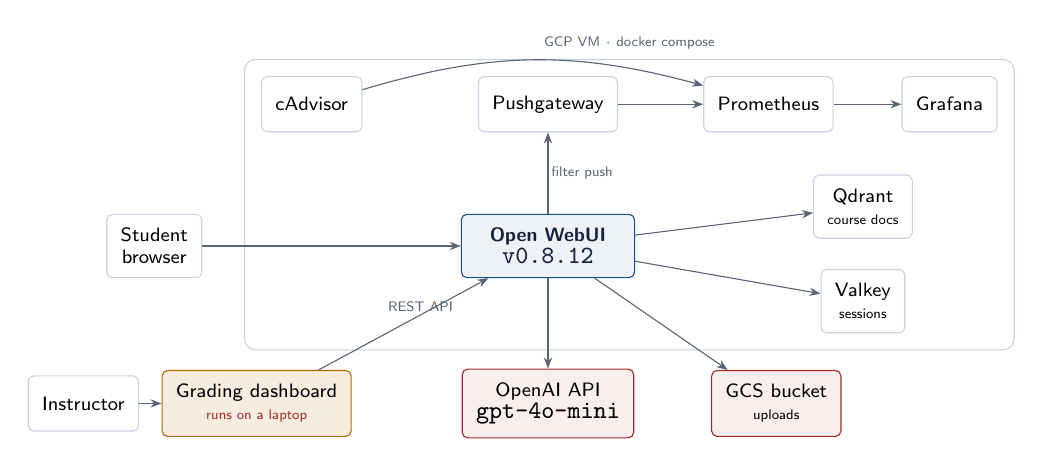
\begin{tikzpicture}[scale=1,every node/.style={transform shape}]
    % --- monitoring band
    \node[box]  at (3.9,4.7) (cad)  {cAdvisor};
    \node[box]  at (6.9,4.7) (pg)   {Pushgateway};
    \node[box]  at (9.7,4.7) (prom) {Prometheus};
    \node[box]  at (12.0,4.7)(graf) {Grafana};
    % --- application band
    \node[box]  at (1.9,2.9) (stu)  {Student\\browser};
    \node[core,minimum width=22mm] at (6.9,2.9) (ow) {Open WebUI\\ \code{v0.8.12}};
    \node[box]  at (10.9,3.4)(qd)   {Qdrant\\ {\tiny course docs}};
    \node[box]  at (10.9,2.2)(rd)   {Valkey\\ {\tiny sessions}};
    % --- external / instructor band
    \node[box,fill=ffcAmber!12,draw=ffcAmber] at (3.2,0.9) (dash)
      {Grading dashboard\\ \textcolor{ffcRed}{\tiny runs on a laptop}};
    \node[box]  at (1.0,0.9) (prof) {Instructor};
    \node[ext]  at (6.9,0.9) (oai)  {OpenAI API\\ \code{gpt-4o-mini}};
    \node[ext]  at (9.8,0.9) (gcs)  {GCS bucket\\ {\tiny uploads}};

    \draw[arr] (stu) -- (ow);
    \draw[arr] (ow) -- (qd);
    \draw[arr] (ow) -- (rd);
    \draw[arr] (ow) -- (oai);
    \draw[arr] (ow) -- (gcs);
    \draw[arr] (ow) -- node[lbl,right]{filter push} (pg);
    \draw[arr] (pg) -- (prom);
    \draw[arr] (cad) to[bend left=16] (prom);   % arc gently over Pushgateway
    \draw[arr] (prom) -- (graf);
    \draw[arr] (prof) -- (dash);
    \draw[arr] (dash) -- node[lbl,above,pos=0.6]{REST API} (ow);
    \begin{scope}[on background layer]
      \node[fit=(cad)(graf)(ow)(qd)(rd)(pg),draw=ffcRule,rounded corners,
            inner sep=6pt,label={[font=\tiny,text=ffcGrey]above:GCP VM $\cdot$ docker compose}] {};
    \end{scope}
  \end{tikzpicture}
  \end{center}
  \vspace{-0.4em}
  {\footnotesize Eight containers on one VM. Retrieval over course documents in Qdrant.
  Chat metrics pushed by a plugin. \bad{The grading dashboard is the outlier --- it is not hosted.}}
  \note{Walk the diagram left to right. Land on the one thing in amber: the professor's tool runs on a laptop. That is workstream A's headline problem.}
\end{frame}

%== 5 =========================================================================
\begin{frame}{The lesson that shaped this project}
  \vspace{-0.3em}
  \begin{columns}[T]
    \begin{column}{0.47\textwidth}
      \textbf{\bad{Before}} --- Spring 2026 and earlier
      \begin{center}
      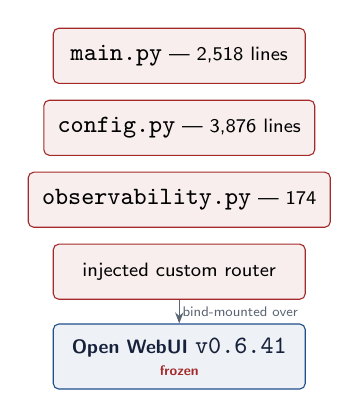
\begin{tikzpicture}
        \node[ext,minimum width=32mm] (a) {\code{main.py} --- 2{,}518 lines};
        \node[ext,minimum width=32mm,below=2mm of a] (b) {\code{config.py} --- 3{,}876 lines};
        \node[ext,minimum width=32mm,below=2mm of b] (c) {\code{observability.py} --- 174};
        \node[ext,minimum width=32mm,below=2mm of c] (d) {injected custom router};
        \node[core,minimum width=32mm,below=3mm of d] (e) {Open WebUI \code{v0.6.41}\\ \textcolor{ffcRed}{\tiny frozen}};
        \draw[arr] (d) -- node[lbl,right]{bind-mounted over} (e);
      \end{tikzpicture}
      \end{center}
      \vspace{2pt}
      {\footnotesize \bad{$\approx$6{,}500 lines} of forked vendor code, re-merged by hand
      on every upgrade. Users reached a feature via a \emph{browser bookmarklet}.}
    \end{column}
    \begin{column}{0.47\textwidth}
      \textbf{\good{After}} --- what we inherited
      \begin{center}
      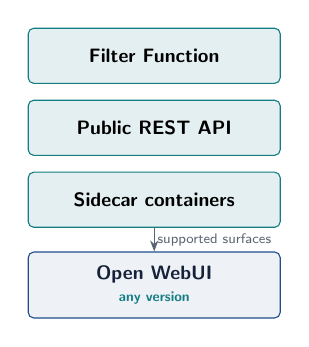
\begin{tikzpicture}
        \node[newb,minimum width=32mm] (f) {Filter Function};
        \node[newb,minimum width=32mm,below=2mm of f] (g) {Public REST API};
        \node[newb,minimum width=32mm,below=2mm of g] (h) {Sidecar containers};
        \node[core,minimum width=32mm,below=3mm of h] (i) {Open WebUI\\ \textcolor{ffcTeal}{\tiny any version}};
        \draw[arr] (h) -- node[lbl,right]{supported surfaces} (i);
      \end{tikzpicture}
      \end{center}
      \vspace{2pt}
      {\footnotesize The \code{Dockerfile} is now \good{one line}. Every customisation
      rides a documented plugin or API surface.}
    \end{column}
  \end{columns}
  \vspace{0.1em}
  \centerline{\small\textit{This is the previous team's real achievement --- and it is why this semester is possible.}}
  \note{Give the last team credit. Six and a half thousand lines of fork to get two features. The bookmarklet detail always lands -- mention it.}
\end{frame}

%== 6 =========================================================================
\begin{frame}{Where it still hurts}
  \vspace{0.2em}
  \begin{center}\footnotesize
  \begin{tabular}{p{5.6cm}p{6.6cm}}
    \toprule
    \textbf{Problem} & \textbf{Consequence} \\
    \midrule
    Pinned to \code{v0.8.12}; upstream ships \code{v0.11.x} & Three minor versions of fixes, features --- and \emph{migrations} --- deferred \\
    Metrics plugin is pasted into the admin UI by hand after every deploy & Deployment is not reproducible; metrics vanish silently \\
    That plugin is synchronous, with blocking network I/O and shared state & On the v0.9+ async core it degrades every concurrent user \\
    \bad{Grading dashboard is not hosted} & A professor needs SSH and a terminal to grade \\
    No CI, no automated smoke test & Past upgrades broke things silently \\
    No alerting on \code{/ready} & An outage was discovered from students \\
    Two RAG stacks, two scoring implementations & Ambiguity about which numbers are canonical \\
    Default \code{admin/admin}; unrotated leaked key & Straightforward security debt \\
    \bottomrule
  \end{tabular}
  \end{center}
  \vspace{0.4em}
  \centerline{\small None of this is exotic. It is the gap between \emph{a system that works} and \emph{a system you can hand over}.}
  \note{Read only three or four rows aloud -- hosted dashboard, no CI, version gap. Close with the "gap between works and handover" line.}
\end{frame}

%== 7 =========================================================================
\sectionslide{Workstream A}{Harden and modernise}{Weeks 1--15 $\cdot$ this must not slip}

%== 8 =========================================================================
\begin{frame}{The compatibility contract}
  \vspace{0.5em}
  \begin{block}{The rule}
    \normalsize Open WebUI is a \hl{dependency}, not a codebase we own. We must be able to
    pull any published release and have the platform work --- with no merge, no patch,
    no re-fork.
  \end{block}
  \vspace{0.6em}
  \begin{columns}[T]
    \begin{column}{0.55\textwidth}
      {\small Every feature must ride a surface that upstream \hl{publishes, documents,
      and versions}.\\[6pt]
      If a feature cannot be built that way, the \emph{feature} is redesigned or dropped.
      The core is never modified.}
    \end{column}
    \begin{column}{0.42\textwidth}
      \begin{block}{The one-sentence test}
        \small \textit{If upstream cut a release tomorrow and we ran it unchanged, would
        this still work?}\\[4pt]
        If the answer needs ``well, as long as they don't change\ldots'', it is forbidden.
      \end{block}
    \end{column}
  \end{columns}
  \note{Slow down here. This is the intellectual core of the deck. The one-sentence test is what they should apply in code review all semester.}
\end{frame}

%== 9 =========================================================================
\begin{frame}{Where we are allowed to build}
  \vspace{0.2em}
  \begin{center}\footnotesize
  \begin{tabular}{llp{6.4cm}}
    \toprule
    & \textbf{Surface} & \textbf{Use it for} \\
    \midrule
    A1 & Environment / admin settings & models, RAG parameters, STT and TTS engines, OTel export \\
    A2 & Filter Functions & observing or lightly rewriting a request in flight \\
    A3 & Pipe Functions & exposing our own logic as a selectable ``model'' \\
    A4 & Action Functions & per-message buttons --- e.g.\ \emph{start a voice session} \\
    A5 & Pipelines server & anything needing its own dependencies, GPU, or heavy compute \\
    A6 & Tools / OpenAPI / MCP & letting the model call our services \\
    A7 & Public REST API & grading extraction, KB sync, \hl{the avatar app} \\
    A8 & Sidecar containers & exporters, our own web applications \\
    A9 & Reverse-proxy composition & TLS, auth, path routing on one hostname \\
    A10 & Knowledge Bases and Skills & course documents and frameworks, professor-editable \\
    \bottomrule
  \end{tabular}
  \end{center}
  \vspace{0.3em}
  \centerline{\small\textbf{Heuristic:} needs to see \emph{inside} a request $\to$ A2--A4. Needs its own runtime $\to$ A5/A8, talking over A7.}
  \note{Do not read the table. Point at A7 and A8 -- those two are what the avatar work will use. The heuristic line is the takeaway.}
\end{frame}

%== 10 ========================================================================
\begin{frame}{What is forbidden --- permanently}
  \vspace{0.3em}
  \begin{center}\footnotesize
  \begin{tabular}{lp{5.9cm}p{5.0cm}}
    \toprule
    & \textbf{Forbidden} & \textbf{Why} \\
    \midrule
    F1 & Mounting or copying anything into \code{/app/backend/open\_webui/} & this \emph{is} the fork \\
    F2 & Adding modules to the \code{open\_webui} package & same, plus coupling to internals \\
    F3 & Building a custom image from modified source & tracks upstream by hand forever \\
    F4 & JavaScript injection into the Svelte frontend & no contract; breaks on any refactor \\
    F5 & Direct SQL against Open WebUI's schema & the schema is private, and \emph{did} change \\
    F6 & Monkeypatching internals from a Function & a fork wearing a plugin costume \\
    F7 & Relying on undocumented endpoints or fields & fine until it isn't; fails silently \\
    F8 & Pinning to an old release to dodge migration work & \bad{this is exactly how v0.6.41 happened} \\
    \bottomrule
  \end{tabular}
  \end{center}
  \vspace{0.4em}
  \centerline{\small It always starts the same way: \textit{``it's just one file, we'll mount it read-only.''}}
  \note{F6 and F8 are the ones teams actually violate. The closing quote is the warning to remember.}
\end{frame}

%== 11 ========================================================================
\begin{frame}{Audit: what we still have to strip out}
  \vspace{0.2em}
  {\footnotesize \good{Good news:} the active stack is already compliant --- no compose file
  mounts anything into Open WebUI's source tree. What remains is peripheral coupling and
  \emph{loaded guns left in the tree.}}
  \vspace{0.5em}
  \begin{center}\footnotesize
  \begin{tabular}{lp{4.8cm}p{5.2cm}l}
    \toprule
    & \textbf{Finding} & \textbf{Action} & \textbf{Risk} \\
    \midrule
    C-1 & the vendor-fork source under \code{legacy/} --- with a README telling you how to re-fork & delete from the tree; leave a tombstone pointing at the commit & \bad{High} \\
    C-2 & \code{--legacy} direct-SQLite flag (a \code{TODO} stub) & delete the flag; REST API is the only path & Med \\
    C-3 & custom \code{build:} context for Open WebUI & replace with a pinned \code{image:}; delete the \code{Dockerfile} & Low \\
    C-4 & metrics filter: sync, blocking I/O, shared state & rewrite async, or retire it for native OTel & \bad{High} \\
    C-6 & \code{:latest} images (Qdrant, cAdvisor) & pin every image & Med \\
    C-7 & Grafana 9.0.0, default \code{admin/admin} & upgrade; remove the default password & \bad{High} \\
    C-8/9 & two RAG stacks, two scoring implementations & pick one canonical each, in writing & Med \\
    C-10 & previously leaked provider key not yet rotated & rotate at the provider; add \code{gitleaks} to CI & \bad{High} \\
    \bottomrule
  \end{tabular}
  \end{center}
  \note{C-1 is the headline: the repo still contains working instructions for re-creating the fork. Deleting it is a five-minute job with outsized value.}
\end{frame}

%== 12 ========================================================================
\begin{frame}{Version debt: what three releases cost us}
  \vspace{0.4em}
  \begin{center}\small
  \begin{tabular}{lp{3.7cm}p{7.0cm}}
    \toprule
    \textbf{Release} & \textbf{Change} & \textbf{What it means for us} \\
    \midrule
    \code{v0.9.0} & backend went \hl{async top to bottom} & \bad{our Filter Function must be migrated} --- sync plugin code with blocking I/O is now actively harmful \\[4pt]
    \code{v0.10.0} & \code{config} table replaced by a per-key table & \bad{one-way migration.} An older instance pointed at a migrated database fails immediately \\[4pt]
    \code{v0.11.0} & additive columns only; \code{psycopg} v3; major UI reorganisation & low migration risk, \hl{high documentation risk} --- every screenshot and click-path we publish is now wrong \\
    \bottomrule
  \end{tabular}
  \end{center}
  \vspace{0.7em}
  \centerline{\small We are on \code{v0.8.12}. \textbf{The longer this waits, the more expensive it gets ---}}
  \centerline{\small\textit{which is precisely the dynamic that produced the v0.6.41 freeze.}}
  \note{The point is not "upgrades are nice". It is that deferred migrations compound, and this project already has the scar to prove it.}
\end{frame}

%== 13 ========================================================================
\begin{frame}{How we will do the upgrade}
  \vspace{0.4em}
  \begin{columns}[T]
    \begin{column}{0.56\textwidth}
      \small
      \begin{enumerate}
        \item Snapshot production --- and \hl{restore the snapshot into the test stack}.
              \textit{A backup you have never restored is not a backup.}
        \item Upgrade the test stack first, on real production data.
        \item Move \hl{one minor version at a time}: 0.8 $\to$ 0.9 $\to$ 0.10 $\to$ 0.11.
              Migrations run sequentially; a single jump makes failures unattributable.
        \item Run the smoke suite at every step. Write the runbook \emph{as you go}.
        \item Decide \hl{SQLite $\to$ PostgreSQL} explicitly, and record the decision either way.
        \item Schedule the production window with the rollback written \emph{before} you start.
        \item Re-shoot every screenshot for the new UI.
      \end{enumerate}
    \end{column}
    \begin{column}{0.40\textwidth}
      \begin{block}{Done when}
        \small
        Production runs the current release.\\[3pt]
        The runbook exists \emph{and was followed}.\\[3pt]
        The smoke suite passes.\\[3pt]
        Docs match what a user actually sees.\\[3pt]
        The rollback is \hl{proven}, not theorised.
      \end{block}
      \vspace{0.4em}
      {\footnotesize \bad{Schedule this outside student deadline weeks.}}
    \end{column}
  \end{columns}
  \note{Step 1 and step 6 are the professional habits worth arguing for. Most teams skip both and get away with it until they don't.}
\end{frame}

%== 14 ========================================================================
\begin{frame}{CI/CD --- and the guard that keeps the fork dead}
  \vspace{0.3em}
  \begin{columns}[T]
    \begin{column}{0.52\textwidth}
      \textbf{\color{ffcBlue}Pipeline, by value per hour spent}
      \begin{enumerate}\small
        \item \textbf{Smoke test on every push} --- bring the stack up, wait for
              \code{/health} then \code{/ready}, send a chat completion, upload a
              document, assert retrieval returns it
        \item \textbf{Fork guard} (below)
        \item \textbf{Secret scanning} --- \code{gitleaks}, including history
        \item \textbf{Lint and unit tests} --- especially on the scoring service:
              \emph{it produces numbers that become grades}
        \item \textbf{Deploy on tag} --- pull, restart, re-smoke, auto-rollback
      \end{enumerate}
    \end{column}
    \begin{column}{0.45\textwidth}
      \begin{block}{The fork guard --- fails the build when\ldots}
        \small
        a compose file mounts into \code{open\_webui/}\\[2pt]
        the image is built from modified source\\[2pt]
        Python opens SQLite against Open WebUI's data\\[2pt]
        \code{gitleaks} finds a credential\\[2pt]
        any image reference ends in \code{:latest}
      \end{block}
      \vspace{0.3em}
      {\footnotesize $\approx$40 lines of grep and one GitHub Action. \hl{This is what makes
      the policy real instead of aspirational.} Build it in Week 2.}
    \end{column}
  \end{columns}
  \note{Emphasise: a policy nobody enforces is a wish. Forty lines of grep converts a document into a constraint.}
\end{frame}

%== 15 ========================================================================
\begin{frame}{Two fixes that change who can use this}
  \vspace{0.4em}
  \begin{columns}[T]
    \begin{column}{0.47\textwidth}
      \textbf{\color{ffcBlue}Host the grading dashboard}\\[4pt]
      {\small Today a professor must SSH into a GCP VM and run a shell script.\\[5pt]
      Containerise the backend, build the frontend to static assets, put Nginx in front with
      TLS and real authentication, and give them a \hl{URL}.\\[5pt]
      \textit{Watch:} make \code{/refresh} asynchronous with visible progress --- it scores
      every question through a paid API.}
      \\[6pt]
      {\footnotesize\good{Done when} a professor grades with no terminal, no VPN, and no help
      from a student.}
    \end{column}
    \begin{column}{0.47\textwidth}
      \textbf{\color{ffcBlue}Observability without manual steps}\\[4pt]
      {\small Chat metrics currently depend on a human pasting Python into an admin form
      after every deployment.\\[5pt]
      Fix the \emph{class} of problem: enable Open WebUI's \hl{native OpenTelemetry export}
      into a collector, and scrape that. Then retire the filter --- or rewrite it async.\\[5pt]
      Add a \code{/ready} uptime check that alerts \emph{a person}, and a memory alert as a
      leading indicator.}
      \\[6pt]
      {\footnotesize\good{Done when} a clean deployment produces metrics with zero manual
      steps, and an induced outage pages someone in five minutes.}
    \end{column}
  \end{columns}
  \note{These two are the highest-adoption-value items in the whole plan. The dashboard one is the difference between a tool that gets used and one that doesn't.}
\end{frame}

%== 16 ========================================================================
\begin{frame}{Remove the ambiguity}
  \vspace{0.5em}
  \begin{columns}[T]
    \begin{column}{0.31\textwidth}
      \begin{block}{Scoring exists twice}
        \small JavaScript and Python, kept in sync by hand.\\[4pt]
        Declare \hl{Python canonical}. Retire the prototype. Add tests that pin the rubric
        arithmetic and ABI weights.
      \end{block}
    \end{column}
    \begin{column}{0.31\textwidth}
      \begin{block}{RAG exists twice}
        \small Native Qdrant (what students use) and a standalone ChromaDB pipeline
        (which nothing uses).\\[4pt]
        Retire it, or promote it behind a \hl{Pipelines server}. Decide in writing.
      \end{block}
    \end{column}
    \begin{column}{0.31\textwidth}
      \begin{block}{Extraction is heuristic}
        \small Student questions are found by punctuation and keywords.\\[4pt]
        \hl{Measure its accuracy} against a hand-labelled sample before trusting the scores
        built on top of it.
      \end{block}
    \end{column}
  \end{columns}
  \vspace{0.9em}
  \centerline{\small Each of these will eventually produce a wrong answer that nobody can explain.}
  \centerline{\small\textit{Dead code with live bugs is a tax --- the citation bug we fixed lived in the stack nobody runs.}}
  \note{The third column is the sleeper. If question extraction is 70 percent accurate, every grade downstream inherits that error, silently.}
\end{frame}

%== 17 ========================================================================
\sectionslide{Workstream B}{Embodied advising}{The new research track $\cdot$ Weeks 3--15}

%== 18 ========================================================================
\begin{frame}{Why typing is not enough}
  \vspace{0.2em}
  \begin{columns}[T]
    \begin{column}{0.5\textwidth}
      {\small FIN 602 exists to prepare students for \hl{a room with a real family in it}.
      \\[8pt]
      That room demands: listening while someone is still talking, hearing hesitation,
      holding eye contact through an uncomfortable question about money, and asking the
      follow-up \emph{out loud} --- without a backspace key.}
    \end{column}
    \begin{column}{0.46\textwidth}
      \begin{block}{The gap}
        \small The platform teaches the \emph{content} of good advising well.\\[4pt]
        It cannot teach the \emph{performance} of it --- because typing removes every one of
        those pressures.\\[4pt]
        A student can draft, delete, and reword for ninety seconds before asking
        \textit{``what happens to the business if something happens to you?''}
      \end{block}
    \end{column}
  \end{columns}
  \vspace{0.8em}
  \begin{block}{This semester's hypothesis --- and it is a hypothesis}
    \small A spoken, face-to-face AI client produces meaningfully better preparation than a
    text chatbot --- and we can \hl{measure whether that is true} with the scoring pipeline
    the platform already has. This track is designed to be allowed to answer \emph{no}.
  \end{block}
  \note{This is the emotional centre of the pitch. Deliver the backspace-key line slowly. Then immediately frame it as testable, not assumed.}
\end{frame}

%== 19 ========================================================================
\begin{frame}{What we are actually building}
  \vspace{0.5em}
  {\small A student opens a link, sees a face, and says out loud:}
  \vspace{0.3em}
  \begin{center}
    \colorbox{ffcMist}{\parbox{0.8\textwidth}{\vspace{3pt}\small\itshape\centering
    ``Hi --- I'm going to ask you a few questions about your family's finances.
    Is that alright?''\vspace{3pt}}}
  \end{center}
  \vspace{0.3em}
  {\small The client on screen \hl{looks at them, nods, and answers in their own voice},
  in character, with their own financial situation --- drawn from the same course documents
  the text bot already uses.\\[4pt]
  If the student interrupts, the client \hl{stops talking}. If the student goes quiet, the
  client waits --- and may eventually prompt them, the way a real, slightly impatient client
  would.\\[4pt]
  At the end, the transcript lands in \hl{the same grading dashboard}, scored on the same
  seven dimensions and the same ABI rubric.}
  \vspace{0.5em}
  \begin{block}{What we are \emph{not} building}
    \small A photorealistic digital human. A likeness of any real person. A replacement for
    the text interface --- text stays. Voice and face are an \emph{additional mode}.
  \end{block}
  \note{Read the quoted line as if speaking to the avatar. The "stops talking" detail is what separates a real prototype from a demo video.}
\end{frame}

%== 20 ========================================================================
\begin{frame}{The constraint dictates the architecture}
  \vspace{0.5em}
  {\small The instinct is to put the avatar \emph{inside} the Open WebUI chat window.}
  \vspace{0.4em}
  \begin{block}{That is forbidden --- F3 and F4 at once}
    \small Open WebUI's frontend is a Svelte application we do not own. Embedding a WebRTC
    video pane in it means forking and re-merging that frontend forever ---
    \bad{precisely the mistake this project spent a semester undoing.}
  \end{block}
  \vspace{0.5em}
  {\small So the constraint decides the design, and the design it produces is \good{better}:}
  \vspace{0.3em}
  \centerline{\small\textbf{The avatar is a companion web application in its own container.}}
  \centerline{\small Open WebUI stays the \hl{brain} (model, RAG, knowledge) and the
  \hl{system of record} (transcripts). We talk to it over the public API.}
  \vspace{0.6em}
  \begin{columns}[T]
    \begin{column}{0.49\textwidth}
      {\footnotesize \good{$\rightarrow$} deploy, roll back, and load-test independently\\
      \good{$\rightarrow$} survives every upstream release by construction}
    \end{column}
    \begin{column}{0.49\textwidth}
      {\footnotesize \good{$\rightarrow$} if we kill the track in December, we delete one container\\
      \good{$\rightarrow$} students and professors keep the interface they know}
    \end{column}
  \end{columns}
  \note{This slide is the argument that the compatibility policy is not bureaucracy -- it produced a better architecture than the instinctive one.}
\end{frame}

%== 21 ========================================================================
\begin{frame}{Reference architecture}
  \vspace{-0.3em}
  \begin{center}
  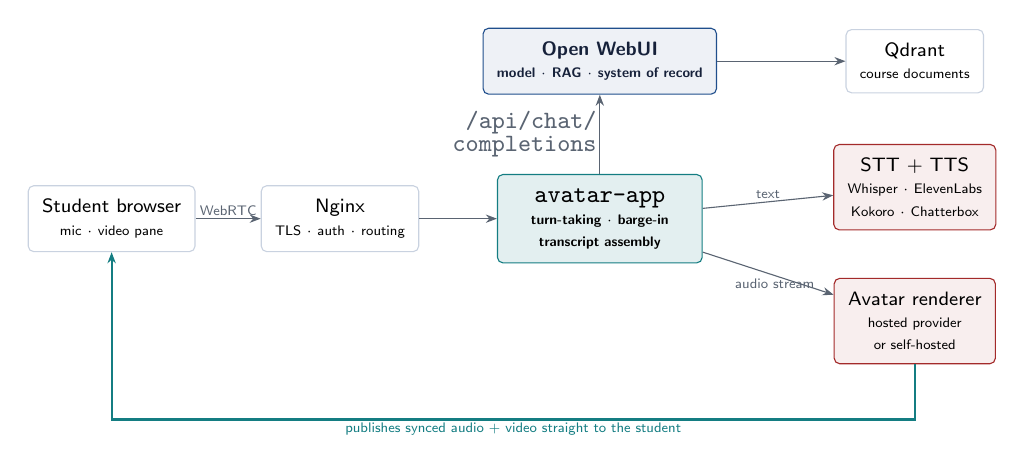
\begin{tikzpicture}[scale=1,every node/.style={transform shape}]
    \node[box]  at (1.7,3.0) (br)  {Student browser\\ {\tiny mic $\cdot$ video pane}};
    \node[box]  at (4.6,3.0) (px)  {Nginx\\ {\tiny TLS $\cdot$ auth $\cdot$ routing}};
    \node[newb,minimum width=26mm] at (7.9,3.0) (app)
        {\code{avatar-app}\\ {\tiny turn-taking $\cdot$ barge-in}\\ {\tiny transcript assembly}};
    \node[core,minimum width=26mm] at (7.9,5.0) (ow)
        {Open WebUI\\ {\tiny model $\cdot$ RAG $\cdot$ system of record}};
    \node[box]  at (11.9,5.0) (qd) {Qdrant\\ {\tiny course documents}};
    \node[ext]  at (11.9,3.4) (stt) {STT + TTS\\ {\tiny Whisper $\cdot$ ElevenLabs}\\ {\tiny Kokoro $\cdot$ Chatterbox}};
    \node[ext]  at (11.9,1.7) (av)  {Avatar renderer\\ {\tiny hosted provider}\\ {\tiny or self-hosted}};

    \draw[arr] (br) -- node[lbl,above]{WebRTC} (px);
    \draw[arr] (px) -- (app);
    \draw[arr] (app) -- node[lbl,left,align=right]{\code{/api/chat/}\\ \code{completions}} (ow);
    \draw[arr] (ow) -- (qd);
    \draw[arr] (app) -- node[lbl,above]{text} (stt);
    \draw[arr] (app) -- node[lbl,below,pos=0.55]{audio stream} (av);
    \draw[arr,draw=ffcTeal,thick] (av.south) -- ++(0,-0.7)
        -| node[lbl,below,pos=0.25,text=ffcTeal]
        {publishes synced audio + video straight to the student} (br.south);
  \end{tikzpicture}
  \end{center}
  \vspace{-0.2em}
  {\footnotesize \good{The pattern that matters:} the renderer is not a step we wait on. It
  \hl{joins the session as its own participant} --- we stream it audio, and it publishes
  finished, lip-synced video directly to the student. That removes a full round trip through
  our server. It is the difference between a video call and a laggy video attachment.}
  \note{Trace the teal arrow. Do not hand-roll WebRTC and turn-taking -- use LiveKit Agents or Pipecat. That is not the semester's research question.}
\end{frame}

%== 22 ========================================================================
\begin{frame}{Latency is the number that decides everything}
  \vspace{0.3em}
  \begin{columns}[T]
    \begin{column}{0.55\textwidth}
      \centering\footnotesize
      \begin{tabular}{lr}
        \toprule
        \textbf{Stage} & \textbf{Realistic} \\
        \midrule
        Voice activity detection / endpointing & 150--300\,ms \\
        Speech to text & 150--300\,ms \\
        \textcolor{ffcRed}{Retrieval (RAG)} & \textcolor{ffcRed}{100--300\,ms} \\
        LLM time-to-first-token & 300--600\,ms \\
        Text to speech, first byte & 150--300\,ms \\
        Avatar render + network & 200--500\,ms \\
        \midrule
        \textbf{First audible syllable} & \textbf{1.0--2.3\,s} \\
        \bottomrule
      \end{tabular}
    \end{column}
    \begin{column}{0.42\textwidth}
      \begin{block}{Targets for this semester}
        \small p50 under \hl{1.2\,s}\\
        p95 under \hl{2.0\,s}\\
        barge-in interrupts within \hl{300\,ms}
      \end{block}
      \vspace{0.3em}
      {\footnotesize Conversation tolerates about a second. Past two, a person stops feeling
      \emph{heard} and starts feeling \emph{processed}.}
    \end{column}
  \end{columns}
  \vspace{0.5em}
  {\footnotesize \bad{The RAG trap:} the text platform retrieves on every turn. In a spoken
  loop that sits directly in the critical path. Strongly consider loading the family scenario
  into the system prompt \emph{once} at session start --- a 2{,}000-token persona brief costs
  less latency than a vector search per turn, every turn.\\[3pt]
  \hl{Instrument every stage separately, in Week 5.} One end-to-end number tells you it is
  slow, not what to fix.}
  \note{The RAG trap is the most useful engineering insight on this slide -- it is counterintuitive and it is where a naive implementation loses half a second per turn.}
\end{frame}

%== 23 ========================================================================
\begin{frame}{Three strategies --- and the one we start with}
  \vspace{0.3em}
  \begin{columns}[T]
    \begin{column}{0.31\textwidth}
      \begin{block}{1. Hosted streaming}
        \footnotesize HeyGen LiveAvatar, Tavus (Phoenix-4), Simli, Anam, bitHuman, Beyond
        Presence, D-ID.\\[4pt]
        Plug into LiveKit or Pipecat; swap providers behind one interface.\\[4pt]
        \textbf{Vendor latency claims are measured under vendor conditions.}
        \hl{Measuring ours is the assignment.}
      \end{block}
    \end{column}
    \begin{column}{0.31\textwidth}
      \begin{block}{2. Self-hosted open source}
        \footnotesize Whisper $\to$ open TTS $\to$ an open lip-sync renderer.\\[4pt]
        \good{For:} no per-minute cost, no student audio leaving our infrastructure.\\[4pt]
        \bad{Against:} needs a GPU we do not have; quality and latency lag; it becomes an
        infrastructure project.
      \end{block}
    \end{column}
    \begin{column}{0.31\textwidth}
      \begin{block}{3. Voice only --- no face}
        \footnotesize Open WebUI \emph{already has} hands-free call mode. STT and TTS are
        configuration, not engineering.\\[4pt]
        Captures much of the benefit --- speaking aloud, no backspace, real-time pressure ---
        at \hl{near-zero build cost}.
      \end{block}
    \end{column}
  \end{columns}
  \vspace{0.7em}
  \begin{block}{Start with \#3, in Week 3}
    \small It de-risks the entire track. If avatars prove too slow, too costly, or too
    fragile, \hl{the course still gains spoken practice this semester.} B0 ships regardless.
  \end{block}
  \note{The strategic point: build the fallback first, and build it in three weeks. That is how you make an ambitious research track safe to attempt.}
\end{frame}

%== 24 ========================================================================
\begin{frame}{What it costs --- and how we stop it running away}
  \vspace{0.4em}
  \begin{columns}[T]
    \begin{column}{0.52\textwidth}
      \centering\footnotesize
      40 students $\times$ 4 sessions $\times$ 15 min $=$ \textbf{40 hours / semester}
      \vspace{0.4em}
      \begin{tabular}{lr}
        \toprule
        \textbf{Line item} & \textbf{Semester} \\
        \midrule
        Avatar streaming ($\sim$\$0.10--0.20/min) & \$240--480 \\
        Speech to text & \$10--30 \\
        Text to speech & \$20--60 \\
        LLM (short spoken turns) & \$15--40 \\
        \midrule
        \textbf{Total} & \textbf{$\approx$\$285--610} \\
        \bottomrule
      \end{tabular}
      \vspace{0.3em}
      {\tiny Checked August 2026. Prices move quarterly --- re-derive at signup and record the date.}
    \end{column}
    \begin{column}{0.45\textwidth}
      \begin{block}{Controls from day one --- not after the first bill}
        \small
        15-minute hard cap, enforced server-side\\[3pt]
        per-student session quota\\[3pt]
        billing alert at 50\% of budget\\[3pt]
        sessions terminate on disconnect\\[3pt]
        a kill switch that needs no redeploy
      \end{block}
      \vspace{0.3em}
      {\footnotesize \bad{Do the arithmetic before advocating self-hosting:} an L4-class GPU
      VM is roughly \$500/month if left running. At 40 hours a semester, \hl{buying beats
      building.} Self-hosting wins on privacy and at scale --- not on cost, here.}
    \end{column}
  \end{columns}
  \note{The self-hosting arithmetic is the slide's punchline. Students instinctively assume open source is cheaper; at this volume it is roughly ten times more expensive.}
\end{frame}

%== 25 ========================================================================
\begin{frame}{How we will evaluate it honestly}
  \vspace{0.3em}
  {\small \good{We already own the outcome measure} --- so use it. Within-subjects,
  counterbalanced: each student practises in two or three modalities with matched scenarios,
  in varied order.}
  \vspace{0.5em}
  \begin{center}\footnotesize
  \begin{tabular}{lp{6.6cm}}
    \toprule
    \textbf{Measure} & \textbf{Question it answers} \\
    \midrule
    7-dimension question quality & do students ask \emph{better} questions when speaking? \\
    ABI trust scores & does modality change how the interaction reads? \\
    Questions asked; session duration & does speaking increase or suppress engagement? \\
    \textcolor{ffcTeal}{Interruptions; talk-time ratio} & \textcolor{ffcTeal}{are students learning to \emph{listen}?} \\
    Hesitation before sensitive questions & does rehearsal reduce discomfort over sessions? \\
    Realism, social presence, anxiety (survey) & is it believable and productive --- or uncanny? \\
    \bottomrule
  \end{tabular}
  \end{center}
  \vspace{0.5em}
  {\footnotesize \bad{Do not over-claim.} The sample is small and the semester is short.
  \textit{``Twelve students, counterbalanced, with these effect sizes and confidence
  intervals''} is a credible result. \textit{``Avatars improve learning''} is not.
  \hl{A well-designed study with an honest negative result is the better deliverable} --- and
  it will be graded that way.}
  \note{The teal row is the genuinely novel contribution: whether a student lets the client finish talking may be a better measure of advising skill than anything the current rubric captures.}
\end{frame}

%== 26 ========================================================================
\begin{frame}{Phases and gates}
  \vspace{0.1em}
  \begin{center}\small
  \begin{tabular}{llp{6.0cm}p{3.6cm}}
    \toprule
    & \textbf{Weeks} & \textbf{Deliverable} & \textbf{Gate} \\
    \midrule
    \textbf{B0} & 3--5 & hands-free spoken practice on Open WebUI's own call mode & \emph{ships regardless} \\[3pt]
    \textbf{B1} & 4--7 & two providers behind one interface, measured on latency, cost, barge-in & \hl{choose --- or recommend stopping} \\[3pt]
    \textbf{B2} & 7--12 & \code{avatar-app} container; transcripts written back into grading & \hl{five students complete a full session} \\[3pt]
    \textbf{B3} & 11--15 & text vs voice vs avatar, measured on the existing rubric & \hl{evidence-backed go / no-go} \\
    \bottomrule
  \end{tabular}
  \end{center}
  \vspace{0.3em}
  \begin{block}{The gates are real}
    \small ``Stop'' is an acceptable outcome at every gate. \bad{``We didn't measure'' is not.}\\[4pt]
    And build the transcript write-back \emph{first} in B2, not last --- an avatar session that
    never reaches the grading dashboard is a demo, not a feature.
  \end{block}
  \note{Make the kill switch explicit and unembarrassing. Research tracks that cannot fail are not research tracks.}
\end{frame}

%== 27 ========================================================================
\begin{frame}{Ethics, privacy, and consent --- settle this in Week 2}
  \vspace{0.4em}
  \begin{columns}[T]
    \begin{column}{0.48\textwidth}
      \small
      \begin{itemize}
        \item Student transcripts are \hl{education records} under FERPA. Adding audio adds a
              biometric-adjacent identifier to that.
        \item \hl{Written informed consent} before any recording: what is captured, where it
              lives, how long, who sees it, how to opt out --- \textbf{without affecting a grade}.
        \item \bad{No likeness of any real person.} Use provider stock avatars under licence.
              Do not clone a professor's face or voice ``as a joke.''
      \end{itemize}
    \end{column}
    \begin{column}{0.48\textwidth}
      \small
      \begin{itemize}
        \item \hl{Disclose the AI.} We are teaching advising, not testing whether students can
              be fooled.
        \item \hl{Minimise data.} Prefer keeping the transcript and discarding the audio.
        \item \hl{Read the vendor's terms} before sending one student's voice: retention,
              training use, sub-processors, region. For an education platform this can
              outweigh a latency win.
        \item Ask about \hl{IRB review} in Week 2 --- approval takes longer than you think.
      \end{itemize}
    \end{column}
  \end{columns}
  \vspace{0.5em}
  \centerline{\small\textit{Settle these before the data exists --- not in Week 13, when it already does.}}
  \note{Do not rush this slide. For a university deployment it is the one that determines whether the project is allowed to run at all.}
\end{frame}

%== 28 ========================================================================
\sectionslide{Execution}{Timeline, roles, and risk}{How the two tracks stay in balance}

%== 29 ========================================================================
\begin{frame}{The semester}
  \vspace{0.2em}
  \begin{center}\scriptsize
  \begin{tabular}{clp{4.9cm}p{4.9cm}}
    \toprule
    \textbf{Wk} & \textbf{Starts} & \textbf{Workstream A --- platform} & \textbf{Workstream B --- avatars} \\
    \midrule
    1 & Aug 24 & set up; run the stack; read the handoff & scope the landscape \\
    2 & Aug 31 & \hl{CI skeleton + fork guard + gitleaks} & requirements; \bad{consent and IRB questions} \\
    3 & Sep 7 & snapshot production; restore into test & \hl{B0: voice session end to end} \\
    4 & Sep 14 & test stack to v0.9.x; migrate the filter & provider shortlist; cost model \\
    5 & Sep 21 & v0.10.x on test & \hl{B0 demo}; latency baseline measured \\
    6 & Sep 28 & v0.11.x on test; docs re-shot & provider \#1 in a bare harness \\
    7 & Oct 5 & \hl{production upgrade window} & provider \#2; head-to-head \\
    8 & Oct 12 & hosted dashboard: container, proxy, TLS & \hl{Gate 1 --- pick, or stop} \\
    9 & Oct 19 & dashboard auth; professor walkthrough & companion app skeleton \\
    10 & Oct 26 & OTel + alerting live & avatar joins the session; barge-in works \\
    11 & Nov 2 & scoring consolidation + tests & transcript write-back \\
    12 & Nov 9 & RAG decision executed & \hl{Gate 2 --- five real sessions} \\
    13 & Nov 16 & performance and cost review & evaluation sessions run \\
    14 & Nov 23 & \textit{(short week)} runbooks and documentation & data analysed \\
    15 & Nov 30 & freeze; handoff written & recommendation drafted \\
    16 & Dec 7 & \multicolumn{2}{l}{\hl{final presentation and handoff}} \\
    \bottomrule
  \end{tabular}
  \end{center}
  \note{Point at weeks 2, 7, and 8. A and B are deliberately interleaved so neither starves. The upgrade lands before the avatar work gets heavy.}
\end{frame}

%== 30 ========================================================================
\begin{frame}{Who owns what}
  \vspace{0.5em}
  \begin{center}\small
  \begin{tabular}{lp{6.9cm}c}
    \toprule
    \textbf{Role} & \textbf{Owns} & \textbf{Track} \\
    \midrule
    Platform / DevOps lead & compose stack, upgrade path, CI/CD, proxy, secrets, backups & A \\
    Backend / integrations & grading service, extraction, scoring, Pipelines & A \\
    Realtime / avatar engineer & STT $\to$ LLM $\to$ TTS $\to$ avatar, latency, provider SDKs & B \\
    Frontend / UX & hosted dashboard, avatar app, session flow & A + B \\
    Data / assessment & evaluation design, metrics, transcript merge, outcomes & A + B \\
    \bottomrule
  \end{tabular}
  \end{center}
  \vspace{0.8em}
  \begin{block}{One duty every member carries}
    \small Review every pull request against the compatibility policy. The question is fixed:\\
    \centerline{\textit{``Which extension surface --- and what happens on the next upstream release?''}}
  \end{block}
  \vspace{0.3em}
  {\footnotesize On a smaller team one person holds two roles. \hl{The roles still exist, and so does the accountability.}}
  \note{Roles are about accountability, not headcount. The shared review duty is what keeps the policy alive when the deadline pressure arrives.}
\end{frame}

%== 31 ========================================================================
\begin{frame}{What could go wrong}
  \vspace{0.2em}
  \begin{center}\footnotesize
  \begin{tabular}{p{5.4cm}cp{5.6cm}}
    \toprule
    \textbf{Risk} & \textbf{Sev} & \textbf{Mitigation} \\
    \midrule
    The v0.10 config migration corrupts production data & \bad{High} & rehearse on a restored snapshot; verify the restore \emph{first}; run outside deadline weeks \\
    \bad{The avatar absorbs the semester and the platform work slips} & \bad{High} & A1 and A2 land before Week 8 --- the timeline front-loads them deliberately \\
    Avatar latency lands at 3+ seconds & Med & measure in Week 5; B0 voice-only ships regardless \\
    Streaming costs surprise the department & Med & caps, quotas, and a billing alarm from day one \\
    Voice and video create privacy exposure & \bad{High} & consent, no real likenesses, documented retention, sign-off \\
    A provider reprices or deprecates mid-semester & Med & provider-agnostic interface; keep the runner-up warm \\
    Somebody proposes embedding video in the chat page & Med & \bad{policy F3/F4 --- refuse.} The companion app exists for this reason \\
    Knowledge is lost at handoff, again & Med & \code{HANDOFF.md} updated continuously, not written in Week 15 \\
    \bottomrule
  \end{tabular}
  \end{center}
  \note{Row two is the one to dwell on. The exciting track will try to eat the boring track, and the boring track is what the course actually depends on.}
\end{frame}

%== 32 ========================================================================
\begin{frame}{Done means done}
  \vspace{0.5em}
  {\small The semester is complete when \hl{all eight} are true:}
  \vspace{0.4em}
  \begin{columns}[T]
    \begin{column}{0.48\textwidth}
      \small
      \begin{enumerate}
        \item Production runs a current release, upgraded via a written, \emph{rehearsed} runbook.
        \item A push runs CI; a tag deploys; a red build blocks the merge.
        \item The fork guard exists and passes --- and no re-forking instructions remain in the tree.
        \item A professor grades from an authenticated URL, with no terminal.
      \end{enumerate}
    \end{column}
    \begin{column}{0.48\textwidth}
      \small
      \begin{enumerate}
        \setcounter{enumi}{4}
        \item Metrics and alerting work from a clean deployment, with zero manual steps.
        \item Scoring and retrieval each have one canonical implementation, with tests.
        \item A working avatar prototype exists, real students used it, and a written
              evaluation backs a go/no-go call.
        \item \code{HANDOFF.md} lets the next team start in Week 1 --- not Week 4.
      \end{enumerate}
    \end{column}
  \end{columns}
  \note{Read these as acceptance criteria, not aspirations. Every one is verifiable by someone who was not in the room.}
\end{frame}

%== 33 ========================================================================
\begin{frame}[plain]
  \begin{tikzpicture}[remember picture,overlay]
    \fill[ffcInk] (current page.south west) rectangle (current page.north east);
    \node[anchor=west,text width=0.82\paperwidth] at ([xshift=1.2cm,yshift=1.5cm]current page.west)
      {\color{white}\LARGE\bfseries The goal is not to finish\\[6pt] FamilyFinanceChat.};
    \node[anchor=west,text width=0.78\paperwidth] at ([xshift=1.2cm,yshift=-0.5cm]current page.west)
      {\color{ffcRule}\large It is to leave a system where the interesting work is
       \textbf{\color{white}the pedagogy}, not \textbf{\color{white}the plumbing}.};
    \node[anchor=west,text width=0.78\paperwidth] at ([xshift=1.2cm,yshift=-2.3cm]current page.west)
      {\color{ffcGrey}\small Every hour spent this semester on upgrades, CI, and hosting is an
       hour a future team does not spend re-learning why the fork was a mistake.};
    \node[anchor=south east] at ([xshift=-1.2cm,yshift=0.9cm]current page.south east)
      {\color{ffcTeal}\small\bfseries Questions?};
  \end{tikzpicture}
  \note{Close on purpose, not on tasks. Then open the floor -- expect questions on avatar cost, on privacy, and on whether the upgrade can wait. It cannot.}
\end{frame}

\end{document}
"
% (build.sh does this for you and names the output ...-notes.pdf)
\ifdefined\SHOWNOTES\setbeameroption{show notes}\fi

\usepackage[T1]{fontenc}
\usepackage[utf8]{inputenc}
\usepackage{helvet}
\renewcommand{\familydefault}{\sfdefault}
\usepackage{microtype}
\usepackage{booktabs}
\usepackage{tikz}
\usepackage{xcolor}
\usetikzlibrary{arrows.meta,positioning,fit,backgrounds,shapes.geometric}

%------------------------------------------------------------------ palette --
\definecolor{ffcInk}{HTML}{16213A}
\definecolor{ffcBlue}{HTML}{1F4E8C}
\definecolor{ffcTeal}{HTML}{147D82}
\definecolor{ffcAmber}{HTML}{B26A00}
\definecolor{ffcRed}{HTML}{A32A2A}
\definecolor{ffcGrey}{HTML}{5A6472}
\definecolor{ffcMist}{HTML}{EEF1F6}
\definecolor{ffcRule}{HTML}{C9D2E0}

%--------------------------------------------------------------------- theme --
\usetheme{default}
\usecolortheme{default}
\setbeamercolor{normal text}{fg=ffcInk}
\setbeamercolor{structure}{fg=ffcBlue}
\setbeamercolor{frametitle}{fg=white,bg=ffcInk}
\setbeamercolor{title}{fg=white}
\setbeamercolor{alerted text}{fg=ffcRed}
\setbeamercolor{block title}{fg=white,bg=ffcBlue}
\setbeamercolor{block body}{fg=ffcInk,bg=ffcMist}
\setbeamerfont{frametitle}{series=\bfseries,size=\large}
\setbeamerfont{title}{series=\bfseries,size=\LARGE}
\setbeamertemplate{navigation symbols}{}
\setbeamertemplate{itemize item}{\color{ffcBlue}\rule[0.35ex]{0.55ex}{0.55ex}}
\setbeamertemplate{itemize subitem}{\color{ffcTeal}\rule[0.35ex]{0.4ex}{0.4ex}}
\setbeamertemplate{section in toc}{\color{ffcInk}\inserttocsectionnumber.~\inserttocsection}

\setbeamertemplate{frametitle}{%
  \nointerlineskip
  \begin{beamercolorbox}[wd=\paperwidth,ht=3.1ex,dp=1.5ex,leftskip=0.9em,rightskip=0.9em]{frametitle}
    \usebeamerfont{frametitle}\insertframetitle%
    \hfill\raisebox{0.2ex}{\scriptsize\color{ffcRule}\insertframenumber}
  \end{beamercolorbox}%
  \vskip0.6ex
}
\setbeamertemplate{footline}{%
  \hbox{\begin{beamercolorbox}[wd=\paperwidth,ht=2.2ex,dp=1ex,leftskip=0.9em,rightskip=0.9em]{}
    {\tiny\color{ffcGrey}FamilyFinanceChat \quad$\cdot$\quad Fall 2026 Project Kickoff}
  \end{beamercolorbox}}
}

%----------------------------------------------------------------- shortcuts --
\newcommand{\hl}[1]{\textcolor{ffcBlue}{\textbf{#1}}}
\newcommand{\bad}[1]{\textcolor{ffcRed}{\textbf{#1}}}
\newcommand{\good}[1]{\textcolor{ffcTeal}{\textbf{#1}}}
\newcommand{\code}[1]{{\small\texttt{#1}}}
% Centred text that WRAPS (plain TeX \centerline does not, and runs off the slide).
\renewcommand{\centerline}[1]{{\par\centering #1\par}}
\newcommand{\yes}{\textcolor{ffcTeal}{\textbf{\checkmark}}}
\newcommand{\no}{\textcolor{ffcRed}{\textbf{\texttimes}}}

% Section divider
\newcommand{\sectionslide}[3]{%
  \begin{frame}[plain]
    \begin{tikzpicture}[remember picture,overlay]
      \fill[ffcInk] (current page.south west) rectangle (current page.north east);
      \node[anchor=west,text width=0.8\paperwidth] at ([xshift=1.2cm,yshift=0.7cm]current page.west)
        {\color{white}\Huge\bfseries #1};
      \node[anchor=west,text width=0.8\paperwidth] at ([xshift=1.2cm,yshift=-0.6cm]current page.west)
        {\color{ffcRule}\large #2};
      \node[anchor=west] at ([xshift=1.2cm,yshift=-1.9cm]current page.west)
        {\color{ffcTeal}\small\bfseries #3};
    \end{tikzpicture}
  \end{frame}
}

% tikz node styles
\tikzset{
  box/.style={rounded corners=2pt,draw=ffcRule,fill=white,inner sep=5pt,
              align=center,font=\scriptsize,minimum height=7mm},
  core/.style={box,fill=ffcMist,draw=ffcBlue,text=ffcInk,font=\scriptsize\bfseries},
  newb/.style={box,fill=ffcTeal!12,draw=ffcTeal,font=\scriptsize\bfseries},
  ext/.style={box,fill=ffcRed!8,draw=ffcRed,font=\scriptsize},
  arr/.style={-{Stealth[length=4pt]},draw=ffcGrey,thin},
  lbl/.style={font=\tiny,text=ffcGrey,inner sep=1pt},
}

%-------------------------------------------------------------------- title ---
\title{FamilyFinanceChat}
\subtitle{Fall 2026: Hardening the Platform, and Giving the Client a Face}
\author{FIN 602 Capstone Engineering Team}
\date{Fall 2026}

\begin{document}

%== 1 =========================================================================
\begin{frame}[plain]
  \begin{tikzpicture}[remember picture,overlay]
    \fill[ffcInk] (current page.south west) rectangle (current page.north east);
    \fill[ffcTeal] ([xshift=1.2cm,yshift=1.35cm]current page.west) rectangle
                   ([xshift=2.6cm,yshift=1.45cm]current page.west);
    \node[anchor=west,text width=0.82\paperwidth] at ([xshift=1.2cm,yshift=0.55cm]current page.west)
      {\color{white}\Huge\bfseries FamilyFinanceChat};
    \node[anchor=west,text width=0.82\paperwidth] at ([xshift=1.2cm,yshift=-0.75cm]current page.west)
      {\color{ffcRule}\Large Fall 2026: hardening the platform,\\[2pt] and giving the client a face};
    \node[anchor=west,text width=0.82\paperwidth] at ([xshift=1.2cm,yshift=-2.4cm]current page.west)
      {\color{ffcGrey}\small FIN 602 Capstone Engineering Team \quad$\cdot$\quad Project kickoff briefing};
  \end{tikzpicture}
  \note{Welcome. Two workstreams this semester: finish making the platform professional, and investigate embodied avatars. Set the tone -- this is a real production system with real users.}
\end{frame}

%== 2 =========================================================================
\begin{frame}{What we will cover}
  \vspace{0.3em}
  \begin{columns}[T,onlytextwidth]
    \begin{column}{0.48\textwidth}
      \textbf{\color{ffcBlue}Part 1 --- The platform}
      \begin{enumerate}\small
        \item Where the system stands today
        \item The lesson that shaped it: the fork
        \item The compatibility contract
        \item What we still have to strip out
        \item Closing the version gap
        \item Making deployment real
      \end{enumerate}
    \end{column}
    \begin{column}{0.48\textwidth}
      \textbf{\color{ffcTeal}Part 2 --- The new bet}
      \begin{enumerate}\small
        \setcounter{enumi}{6}
        \item Why typing is not enough
        \item Avatars: the target experience
        \item Architecture, latency, and cost
        \item How we will evaluate it honestly
        \item Timeline, roles, and risks
      \end{enumerate}
    \end{column}
  \end{columns}
  \vspace{0.9em}
  \begin{block}{The one rule that governs everything}
    \small We never modify Open WebUI's core. If a feature cannot be built on a published
    extension surface, the feature changes --- not the core.
  \end{block}
  \note{Two halves. Flag the rule early -- it recurs in every architectural decision, including the avatar design.}
\end{frame}

%== 3 =========================================================================
\begin{frame}{The problem this platform solves}
  \vspace{0.4em}
  \begin{columns}[T]
    \begin{column}{0.52\textwidth}
      \textbf{\color{ffcBlue}For students}\\[3pt]
      {\small FIN 602 students must practise client-facing financial advising before
      they sit across from a real family.\\[5pt]
      Human role-players do not scale: scheduling bottlenecks, inconsistent
      scenarios, uneven feedback.}
      \\[10pt]
      \textbf{\color{ffcBlue}For instructors}\\[3pt]
      {\small Reading every transcript by hand does not scale either.}
    \end{column}
    \begin{column}{0.44\textwidth}
      \begin{block}{What we built}
        \small
        Unlimited, on-demand AI role-play against realistic family scenarios ---
        grounded in course documents.
        \\[5pt]
        Automated scoring of student questions on \hl{seven quality dimensions}
        and an \hl{Ability--Benevolence--Integrity} trust rubric.
        \\[5pt]
        A grading dashboard that turns transcripts into per-student feedback.
      \end{block}
    \end{column}
  \end{columns}
  \note{Ground the audience in purpose before architecture. Scale + consistency is the value proposition. ABI is the pedagogical differentiator.}
\end{frame}

%== 4 =========================================================================
\begin{frame}{The system today}
  \vspace{-0.2em}
  \begin{center}
  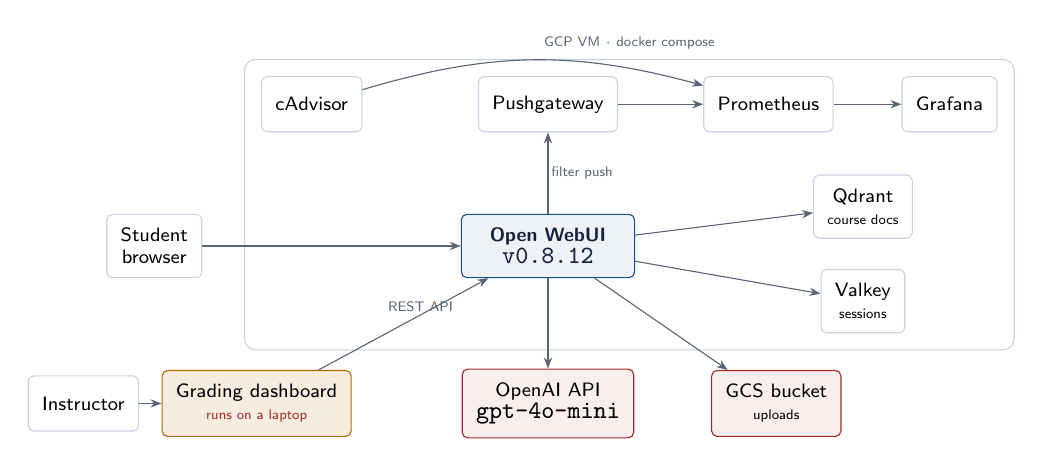
\begin{tikzpicture}[scale=1,every node/.style={transform shape}]
    % --- monitoring band
    \node[box]  at (3.9,4.7) (cad)  {cAdvisor};
    \node[box]  at (6.9,4.7) (pg)   {Pushgateway};
    \node[box]  at (9.7,4.7) (prom) {Prometheus};
    \node[box]  at (12.0,4.7)(graf) {Grafana};
    % --- application band
    \node[box]  at (1.9,2.9) (stu)  {Student\\browser};
    \node[core,minimum width=22mm] at (6.9,2.9) (ow) {Open WebUI\\ \code{v0.8.12}};
    \node[box]  at (10.9,3.4)(qd)   {Qdrant\\ {\tiny course docs}};
    \node[box]  at (10.9,2.2)(rd)   {Valkey\\ {\tiny sessions}};
    % --- external / instructor band
    \node[box,fill=ffcAmber!12,draw=ffcAmber] at (3.2,0.9) (dash)
      {Grading dashboard\\ \textcolor{ffcRed}{\tiny runs on a laptop}};
    \node[box]  at (1.0,0.9) (prof) {Instructor};
    \node[ext]  at (6.9,0.9) (oai)  {OpenAI API\\ \code{gpt-4o-mini}};
    \node[ext]  at (9.8,0.9) (gcs)  {GCS bucket\\ {\tiny uploads}};

    \draw[arr] (stu) -- (ow);
    \draw[arr] (ow) -- (qd);
    \draw[arr] (ow) -- (rd);
    \draw[arr] (ow) -- (oai);
    \draw[arr] (ow) -- (gcs);
    \draw[arr] (ow) -- node[lbl,right]{filter push} (pg);
    \draw[arr] (pg) -- (prom);
    \draw[arr] (cad) to[bend left=16] (prom);   % arc gently over Pushgateway
    \draw[arr] (prom) -- (graf);
    \draw[arr] (prof) -- (dash);
    \draw[arr] (dash) -- node[lbl,above,pos=0.6]{REST API} (ow);
    \begin{scope}[on background layer]
      \node[fit=(cad)(graf)(ow)(qd)(rd)(pg),draw=ffcRule,rounded corners,
            inner sep=6pt,label={[font=\tiny,text=ffcGrey]above:GCP VM $\cdot$ docker compose}] {};
    \end{scope}
  \end{tikzpicture}
  \end{center}
  \vspace{-0.4em}
  {\footnotesize Eight containers on one VM. Retrieval over course documents in Qdrant.
  Chat metrics pushed by a plugin. \bad{The grading dashboard is the outlier --- it is not hosted.}}
  \note{Walk the diagram left to right. Land on the one thing in amber: the professor's tool runs on a laptop. That is workstream A's headline problem.}
\end{frame}

%== 5 =========================================================================
\begin{frame}{The lesson that shaped this project}
  \vspace{-0.3em}
  \begin{columns}[T]
    \begin{column}{0.47\textwidth}
      \textbf{\bad{Before}} --- Spring 2026 and earlier
      \begin{center}
      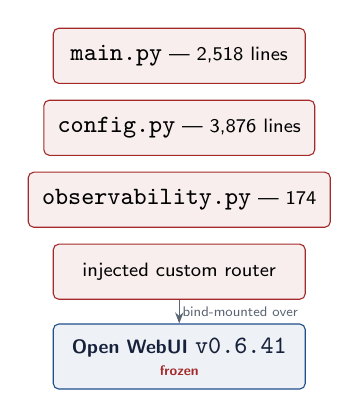
\begin{tikzpicture}
        \node[ext,minimum width=32mm] (a) {\code{main.py} --- 2{,}518 lines};
        \node[ext,minimum width=32mm,below=2mm of a] (b) {\code{config.py} --- 3{,}876 lines};
        \node[ext,minimum width=32mm,below=2mm of b] (c) {\code{observability.py} --- 174};
        \node[ext,minimum width=32mm,below=2mm of c] (d) {injected custom router};
        \node[core,minimum width=32mm,below=3mm of d] (e) {Open WebUI \code{v0.6.41}\\ \textcolor{ffcRed}{\tiny frozen}};
        \draw[arr] (d) -- node[lbl,right]{bind-mounted over} (e);
      \end{tikzpicture}
      \end{center}
      \vspace{2pt}
      {\footnotesize \bad{$\approx$6{,}500 lines} of forked vendor code, re-merged by hand
      on every upgrade. Users reached a feature via a \emph{browser bookmarklet}.}
    \end{column}
    \begin{column}{0.47\textwidth}
      \textbf{\good{After}} --- what we inherited
      \begin{center}
      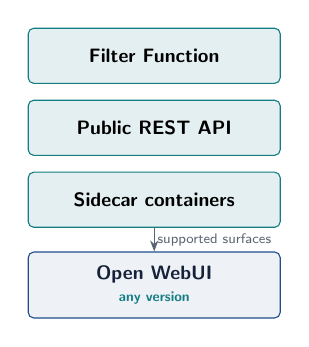
\begin{tikzpicture}
        \node[newb,minimum width=32mm] (f) {Filter Function};
        \node[newb,minimum width=32mm,below=2mm of f] (g) {Public REST API};
        \node[newb,minimum width=32mm,below=2mm of g] (h) {Sidecar containers};
        \node[core,minimum width=32mm,below=3mm of h] (i) {Open WebUI\\ \textcolor{ffcTeal}{\tiny any version}};
        \draw[arr] (h) -- node[lbl,right]{supported surfaces} (i);
      \end{tikzpicture}
      \end{center}
      \vspace{2pt}
      {\footnotesize The \code{Dockerfile} is now \good{one line}. Every customisation
      rides a documented plugin or API surface.}
    \end{column}
  \end{columns}
  \vspace{0.1em}
  \centerline{\small\textit{This is the previous team's real achievement --- and it is why this semester is possible.}}
  \note{Give the last team credit. Six and a half thousand lines of fork to get two features. The bookmarklet detail always lands -- mention it.}
\end{frame}

%== 6 =========================================================================
\begin{frame}{Where it still hurts}
  \vspace{0.2em}
  \begin{center}\footnotesize
  \begin{tabular}{p{5.6cm}p{6.6cm}}
    \toprule
    \textbf{Problem} & \textbf{Consequence} \\
    \midrule
    Pinned to \code{v0.8.12}; upstream ships \code{v0.11.x} & Three minor versions of fixes, features --- and \emph{migrations} --- deferred \\
    Metrics plugin is pasted into the admin UI by hand after every deploy & Deployment is not reproducible; metrics vanish silently \\
    That plugin is synchronous, with blocking network I/O and shared state & On the v0.9+ async core it degrades every concurrent user \\
    \bad{Grading dashboard is not hosted} & A professor needs SSH and a terminal to grade \\
    No CI, no automated smoke test & Past upgrades broke things silently \\
    No alerting on \code{/ready} & An outage was discovered from students \\
    Two RAG stacks, two scoring implementations & Ambiguity about which numbers are canonical \\
    Default \code{admin/admin}; unrotated leaked key & Straightforward security debt \\
    \bottomrule
  \end{tabular}
  \end{center}
  \vspace{0.4em}
  \centerline{\small None of this is exotic. It is the gap between \emph{a system that works} and \emph{a system you can hand over}.}
  \note{Read only three or four rows aloud -- hosted dashboard, no CI, version gap. Close with the "gap between works and handover" line.}
\end{frame}

%== 7 =========================================================================
\sectionslide{Workstream A}{Harden and modernise}{Weeks 1--15 $\cdot$ this must not slip}

%== 8 =========================================================================
\begin{frame}{The compatibility contract}
  \vspace{0.5em}
  \begin{block}{The rule}
    \normalsize Open WebUI is a \hl{dependency}, not a codebase we own. We must be able to
    pull any published release and have the platform work --- with no merge, no patch,
    no re-fork.
  \end{block}
  \vspace{0.6em}
  \begin{columns}[T]
    \begin{column}{0.55\textwidth}
      {\small Every feature must ride a surface that upstream \hl{publishes, documents,
      and versions}.\\[6pt]
      If a feature cannot be built that way, the \emph{feature} is redesigned or dropped.
      The core is never modified.}
    \end{column}
    \begin{column}{0.42\textwidth}
      \begin{block}{The one-sentence test}
        \small \textit{If upstream cut a release tomorrow and we ran it unchanged, would
        this still work?}\\[4pt]
        If the answer needs ``well, as long as they don't change\ldots'', it is forbidden.
      \end{block}
    \end{column}
  \end{columns}
  \note{Slow down here. This is the intellectual core of the deck. The one-sentence test is what they should apply in code review all semester.}
\end{frame}

%== 9 =========================================================================
\begin{frame}{Where we are allowed to build}
  \vspace{0.2em}
  \begin{center}\footnotesize
  \begin{tabular}{llp{6.4cm}}
    \toprule
    & \textbf{Surface} & \textbf{Use it for} \\
    \midrule
    A1 & Environment / admin settings & models, RAG parameters, STT and TTS engines, OTel export \\
    A2 & Filter Functions & observing or lightly rewriting a request in flight \\
    A3 & Pipe Functions & exposing our own logic as a selectable ``model'' \\
    A4 & Action Functions & per-message buttons --- e.g.\ \emph{start a voice session} \\
    A5 & Pipelines server & anything needing its own dependencies, GPU, or heavy compute \\
    A6 & Tools / OpenAPI / MCP & letting the model call our services \\
    A7 & Public REST API & grading extraction, KB sync, \hl{the avatar app} \\
    A8 & Sidecar containers & exporters, our own web applications \\
    A9 & Reverse-proxy composition & TLS, auth, path routing on one hostname \\
    A10 & Knowledge Bases and Skills & course documents and frameworks, professor-editable \\
    \bottomrule
  \end{tabular}
  \end{center}
  \vspace{0.3em}
  \centerline{\small\textbf{Heuristic:} needs to see \emph{inside} a request $\to$ A2--A4. Needs its own runtime $\to$ A5/A8, talking over A7.}
  \note{Do not read the table. Point at A7 and A8 -- those two are what the avatar work will use. The heuristic line is the takeaway.}
\end{frame}

%== 10 ========================================================================
\begin{frame}{What is forbidden --- permanently}
  \vspace{0.3em}
  \begin{center}\footnotesize
  \begin{tabular}{lp{5.9cm}p{5.0cm}}
    \toprule
    & \textbf{Forbidden} & \textbf{Why} \\
    \midrule
    F1 & Mounting or copying anything into \code{/app/backend/open\_webui/} & this \emph{is} the fork \\
    F2 & Adding modules to the \code{open\_webui} package & same, plus coupling to internals \\
    F3 & Building a custom image from modified source & tracks upstream by hand forever \\
    F4 & JavaScript injection into the Svelte frontend & no contract; breaks on any refactor \\
    F5 & Direct SQL against Open WebUI's schema & the schema is private, and \emph{did} change \\
    F6 & Monkeypatching internals from a Function & a fork wearing a plugin costume \\
    F7 & Relying on undocumented endpoints or fields & fine until it isn't; fails silently \\
    F8 & Pinning to an old release to dodge migration work & \bad{this is exactly how v0.6.41 happened} \\
    \bottomrule
  \end{tabular}
  \end{center}
  \vspace{0.4em}
  \centerline{\small It always starts the same way: \textit{``it's just one file, we'll mount it read-only.''}}
  \note{F6 and F8 are the ones teams actually violate. The closing quote is the warning to remember.}
\end{frame}

%== 11 ========================================================================
\begin{frame}{Audit: what we still have to strip out}
  \vspace{0.2em}
  {\footnotesize \good{Good news:} the active stack is already compliant --- no compose file
  mounts anything into Open WebUI's source tree. What remains is peripheral coupling and
  \emph{loaded guns left in the tree.}}
  \vspace{0.5em}
  \begin{center}\footnotesize
  \begin{tabular}{lp{4.8cm}p{5.2cm}l}
    \toprule
    & \textbf{Finding} & \textbf{Action} & \textbf{Risk} \\
    \midrule
    C-1 & the vendor-fork source under \code{legacy/} --- with a README telling you how to re-fork & delete from the tree; leave a tombstone pointing at the commit & \bad{High} \\
    C-2 & \code{--legacy} direct-SQLite flag (a \code{TODO} stub) & delete the flag; REST API is the only path & Med \\
    C-3 & custom \code{build:} context for Open WebUI & replace with a pinned \code{image:}; delete the \code{Dockerfile} & Low \\
    C-4 & metrics filter: sync, blocking I/O, shared state & rewrite async, or retire it for native OTel & \bad{High} \\
    C-6 & \code{:latest} images (Qdrant, cAdvisor) & pin every image & Med \\
    C-7 & Grafana 9.0.0, default \code{admin/admin} & upgrade; remove the default password & \bad{High} \\
    C-8/9 & two RAG stacks, two scoring implementations & pick one canonical each, in writing & Med \\
    C-10 & previously leaked provider key not yet rotated & rotate at the provider; add \code{gitleaks} to CI & \bad{High} \\
    \bottomrule
  \end{tabular}
  \end{center}
  \note{C-1 is the headline: the repo still contains working instructions for re-creating the fork. Deleting it is a five-minute job with outsized value.}
\end{frame}

%== 12 ========================================================================
\begin{frame}{Version debt: what three releases cost us}
  \vspace{0.4em}
  \begin{center}\small
  \begin{tabular}{lp{3.7cm}p{7.0cm}}
    \toprule
    \textbf{Release} & \textbf{Change} & \textbf{What it means for us} \\
    \midrule
    \code{v0.9.0} & backend went \hl{async top to bottom} & \bad{our Filter Function must be migrated} --- sync plugin code with blocking I/O is now actively harmful \\[4pt]
    \code{v0.10.0} & \code{config} table replaced by a per-key table & \bad{one-way migration.} An older instance pointed at a migrated database fails immediately \\[4pt]
    \code{v0.11.0} & additive columns only; \code{psycopg} v3; major UI reorganisation & low migration risk, \hl{high documentation risk} --- every screenshot and click-path we publish is now wrong \\
    \bottomrule
  \end{tabular}
  \end{center}
  \vspace{0.7em}
  \centerline{\small We are on \code{v0.8.12}. \textbf{The longer this waits, the more expensive it gets ---}}
  \centerline{\small\textit{which is precisely the dynamic that produced the v0.6.41 freeze.}}
  \note{The point is not "upgrades are nice". It is that deferred migrations compound, and this project already has the scar to prove it.}
\end{frame}

%== 13 ========================================================================
\begin{frame}{How we will do the upgrade}
  \vspace{0.4em}
  \begin{columns}[T]
    \begin{column}{0.56\textwidth}
      \small
      \begin{enumerate}
        \item Snapshot production --- and \hl{restore the snapshot into the test stack}.
              \textit{A backup you have never restored is not a backup.}
        \item Upgrade the test stack first, on real production data.
        \item Move \hl{one minor version at a time}: 0.8 $\to$ 0.9 $\to$ 0.10 $\to$ 0.11.
              Migrations run sequentially; a single jump makes failures unattributable.
        \item Run the smoke suite at every step. Write the runbook \emph{as you go}.
        \item Decide \hl{SQLite $\to$ PostgreSQL} explicitly, and record the decision either way.
        \item Schedule the production window with the rollback written \emph{before} you start.
        \item Re-shoot every screenshot for the new UI.
      \end{enumerate}
    \end{column}
    \begin{column}{0.40\textwidth}
      \begin{block}{Done when}
        \small
        Production runs the current release.\\[3pt]
        The runbook exists \emph{and was followed}.\\[3pt]
        The smoke suite passes.\\[3pt]
        Docs match what a user actually sees.\\[3pt]
        The rollback is \hl{proven}, not theorised.
      \end{block}
      \vspace{0.4em}
      {\footnotesize \bad{Schedule this outside student deadline weeks.}}
    \end{column}
  \end{columns}
  \note{Step 1 and step 6 are the professional habits worth arguing for. Most teams skip both and get away with it until they don't.}
\end{frame}

%== 14 ========================================================================
\begin{frame}{CI/CD --- and the guard that keeps the fork dead}
  \vspace{0.3em}
  \begin{columns}[T]
    \begin{column}{0.52\textwidth}
      \textbf{\color{ffcBlue}Pipeline, by value per hour spent}
      \begin{enumerate}\small
        \item \textbf{Smoke test on every push} --- bring the stack up, wait for
              \code{/health} then \code{/ready}, send a chat completion, upload a
              document, assert retrieval returns it
        \item \textbf{Fork guard} (below)
        \item \textbf{Secret scanning} --- \code{gitleaks}, including history
        \item \textbf{Lint and unit tests} --- especially on the scoring service:
              \emph{it produces numbers that become grades}
        \item \textbf{Deploy on tag} --- pull, restart, re-smoke, auto-rollback
      \end{enumerate}
    \end{column}
    \begin{column}{0.45\textwidth}
      \begin{block}{The fork guard --- fails the build when\ldots}
        \small
        a compose file mounts into \code{open\_webui/}\\[2pt]
        the image is built from modified source\\[2pt]
        Python opens SQLite against Open WebUI's data\\[2pt]
        \code{gitleaks} finds a credential\\[2pt]
        any image reference ends in \code{:latest}
      \end{block}
      \vspace{0.3em}
      {\footnotesize $\approx$40 lines of grep and one GitHub Action. \hl{This is what makes
      the policy real instead of aspirational.} Build it in Week 2.}
    \end{column}
  \end{columns}
  \note{Emphasise: a policy nobody enforces is a wish. Forty lines of grep converts a document into a constraint.}
\end{frame}

%== 15 ========================================================================
\begin{frame}{Two fixes that change who can use this}
  \vspace{0.4em}
  \begin{columns}[T]
    \begin{column}{0.47\textwidth}
      \textbf{\color{ffcBlue}Host the grading dashboard}\\[4pt]
      {\small Today a professor must SSH into a GCP VM and run a shell script.\\[5pt]
      Containerise the backend, build the frontend to static assets, put Nginx in front with
      TLS and real authentication, and give them a \hl{URL}.\\[5pt]
      \textit{Watch:} make \code{/refresh} asynchronous with visible progress --- it scores
      every question through a paid API.}
      \\[6pt]
      {\footnotesize\good{Done when} a professor grades with no terminal, no VPN, and no help
      from a student.}
    \end{column}
    \begin{column}{0.47\textwidth}
      \textbf{\color{ffcBlue}Observability without manual steps}\\[4pt]
      {\small Chat metrics currently depend on a human pasting Python into an admin form
      after every deployment.\\[5pt]
      Fix the \emph{class} of problem: enable Open WebUI's \hl{native OpenTelemetry export}
      into a collector, and scrape that. Then retire the filter --- or rewrite it async.\\[5pt]
      Add a \code{/ready} uptime check that alerts \emph{a person}, and a memory alert as a
      leading indicator.}
      \\[6pt]
      {\footnotesize\good{Done when} a clean deployment produces metrics with zero manual
      steps, and an induced outage pages someone in five minutes.}
    \end{column}
  \end{columns}
  \note{These two are the highest-adoption-value items in the whole plan. The dashboard one is the difference between a tool that gets used and one that doesn't.}
\end{frame}

%== 16 ========================================================================
\begin{frame}{Remove the ambiguity}
  \vspace{0.5em}
  \begin{columns}[T]
    \begin{column}{0.31\textwidth}
      \begin{block}{Scoring exists twice}
        \small JavaScript and Python, kept in sync by hand.\\[4pt]
        Declare \hl{Python canonical}. Retire the prototype. Add tests that pin the rubric
        arithmetic and ABI weights.
      \end{block}
    \end{column}
    \begin{column}{0.31\textwidth}
      \begin{block}{RAG exists twice}
        \small Native Qdrant (what students use) and a standalone ChromaDB pipeline
        (which nothing uses).\\[4pt]
        Retire it, or promote it behind a \hl{Pipelines server}. Decide in writing.
      \end{block}
    \end{column}
    \begin{column}{0.31\textwidth}
      \begin{block}{Extraction is heuristic}
        \small Student questions are found by punctuation and keywords.\\[4pt]
        \hl{Measure its accuracy} against a hand-labelled sample before trusting the scores
        built on top of it.
      \end{block}
    \end{column}
  \end{columns}
  \vspace{0.9em}
  \centerline{\small Each of these will eventually produce a wrong answer that nobody can explain.}
  \centerline{\small\textit{Dead code with live bugs is a tax --- the citation bug we fixed lived in the stack nobody runs.}}
  \note{The third column is the sleeper. If question extraction is 70 percent accurate, every grade downstream inherits that error, silently.}
\end{frame}

%== 17 ========================================================================
\sectionslide{Workstream B}{Embodied advising}{The new research track $\cdot$ Weeks 3--15}

%== 18 ========================================================================
\begin{frame}{Why typing is not enough}
  \vspace{0.2em}
  \begin{columns}[T]
    \begin{column}{0.5\textwidth}
      {\small FIN 602 exists to prepare students for \hl{a room with a real family in it}.
      \\[8pt]
      That room demands: listening while someone is still talking, hearing hesitation,
      holding eye contact through an uncomfortable question about money, and asking the
      follow-up \emph{out loud} --- without a backspace key.}
    \end{column}
    \begin{column}{0.46\textwidth}
      \begin{block}{The gap}
        \small The platform teaches the \emph{content} of good advising well.\\[4pt]
        It cannot teach the \emph{performance} of it --- because typing removes every one of
        those pressures.\\[4pt]
        A student can draft, delete, and reword for ninety seconds before asking
        \textit{``what happens to the business if something happens to you?''}
      \end{block}
    \end{column}
  \end{columns}
  \vspace{0.8em}
  \begin{block}{This semester's hypothesis --- and it is a hypothesis}
    \small A spoken, face-to-face AI client produces meaningfully better preparation than a
    text chatbot --- and we can \hl{measure whether that is true} with the scoring pipeline
    the platform already has. This track is designed to be allowed to answer \emph{no}.
  \end{block}
  \note{This is the emotional centre of the pitch. Deliver the backspace-key line slowly. Then immediately frame it as testable, not assumed.}
\end{frame}

%== 19 ========================================================================
\begin{frame}{What we are actually building}
  \vspace{0.5em}
  {\small A student opens a link, sees a face, and says out loud:}
  \vspace{0.3em}
  \begin{center}
    \colorbox{ffcMist}{\parbox{0.8\textwidth}{\vspace{3pt}\small\itshape\centering
    ``Hi --- I'm going to ask you a few questions about your family's finances.
    Is that alright?''\vspace{3pt}}}
  \end{center}
  \vspace{0.3em}
  {\small The client on screen \hl{looks at them, nods, and answers in their own voice},
  in character, with their own financial situation --- drawn from the same course documents
  the text bot already uses.\\[4pt]
  If the student interrupts, the client \hl{stops talking}. If the student goes quiet, the
  client waits --- and may eventually prompt them, the way a real, slightly impatient client
  would.\\[4pt]
  At the end, the transcript lands in \hl{the same grading dashboard}, scored on the same
  seven dimensions and the same ABI rubric.}
  \vspace{0.5em}
  \begin{block}{What we are \emph{not} building}
    \small A photorealistic digital human. A likeness of any real person. A replacement for
    the text interface --- text stays. Voice and face are an \emph{additional mode}.
  \end{block}
  \note{Read the quoted line as if speaking to the avatar. The "stops talking" detail is what separates a real prototype from a demo video.}
\end{frame}

%== 20 ========================================================================
\begin{frame}{The constraint dictates the architecture}
  \vspace{0.5em}
  {\small The instinct is to put the avatar \emph{inside} the Open WebUI chat window.}
  \vspace{0.4em}
  \begin{block}{That is forbidden --- F3 and F4 at once}
    \small Open WebUI's frontend is a Svelte application we do not own. Embedding a WebRTC
    video pane in it means forking and re-merging that frontend forever ---
    \bad{precisely the mistake this project spent a semester undoing.}
  \end{block}
  \vspace{0.5em}
  {\small So the constraint decides the design, and the design it produces is \good{better}:}
  \vspace{0.3em}
  \centerline{\small\textbf{The avatar is a companion web application in its own container.}}
  \centerline{\small Open WebUI stays the \hl{brain} (model, RAG, knowledge) and the
  \hl{system of record} (transcripts). We talk to it over the public API.}
  \vspace{0.6em}
  \begin{columns}[T]
    \begin{column}{0.49\textwidth}
      {\footnotesize \good{$\rightarrow$} deploy, roll back, and load-test independently\\
      \good{$\rightarrow$} survives every upstream release by construction}
    \end{column}
    \begin{column}{0.49\textwidth}
      {\footnotesize \good{$\rightarrow$} if we kill the track in December, we delete one container\\
      \good{$\rightarrow$} students and professors keep the interface they know}
    \end{column}
  \end{columns}
  \note{This slide is the argument that the compatibility policy is not bureaucracy -- it produced a better architecture than the instinctive one.}
\end{frame}

%== 21 ========================================================================
\begin{frame}{Reference architecture}
  \vspace{-0.3em}
  \begin{center}
  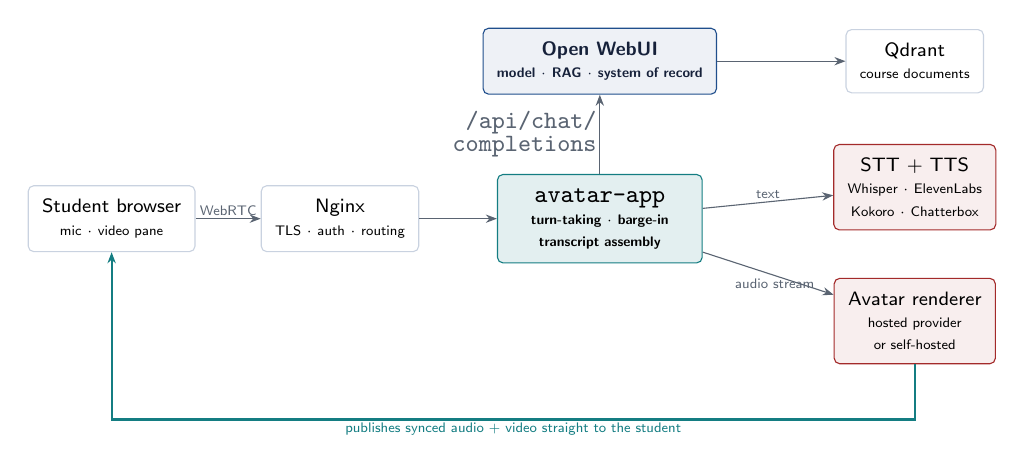
\begin{tikzpicture}[scale=1,every node/.style={transform shape}]
    \node[box]  at (1.7,3.0) (br)  {Student browser\\ {\tiny mic $\cdot$ video pane}};
    \node[box]  at (4.6,3.0) (px)  {Nginx\\ {\tiny TLS $\cdot$ auth $\cdot$ routing}};
    \node[newb,minimum width=26mm] at (7.9,3.0) (app)
        {\code{avatar-app}\\ {\tiny turn-taking $\cdot$ barge-in}\\ {\tiny transcript assembly}};
    \node[core,minimum width=26mm] at (7.9,5.0) (ow)
        {Open WebUI\\ {\tiny model $\cdot$ RAG $\cdot$ system of record}};
    \node[box]  at (11.9,5.0) (qd) {Qdrant\\ {\tiny course documents}};
    \node[ext]  at (11.9,3.4) (stt) {STT + TTS\\ {\tiny Whisper $\cdot$ ElevenLabs}\\ {\tiny Kokoro $\cdot$ Chatterbox}};
    \node[ext]  at (11.9,1.7) (av)  {Avatar renderer\\ {\tiny hosted provider}\\ {\tiny or self-hosted}};

    \draw[arr] (br) -- node[lbl,above]{WebRTC} (px);
    \draw[arr] (px) -- (app);
    \draw[arr] (app) -- node[lbl,left,align=right]{\code{/api/chat/}\\ \code{completions}} (ow);
    \draw[arr] (ow) -- (qd);
    \draw[arr] (app) -- node[lbl,above]{text} (stt);
    \draw[arr] (app) -- node[lbl,below,pos=0.55]{audio stream} (av);
    \draw[arr,draw=ffcTeal,thick] (av.south) -- ++(0,-0.7)
        -| node[lbl,below,pos=0.25,text=ffcTeal]
        {publishes synced audio + video straight to the student} (br.south);
  \end{tikzpicture}
  \end{center}
  \vspace{-0.2em}
  {\footnotesize \good{The pattern that matters:} the renderer is not a step we wait on. It
  \hl{joins the session as its own participant} --- we stream it audio, and it publishes
  finished, lip-synced video directly to the student. That removes a full round trip through
  our server. It is the difference between a video call and a laggy video attachment.}
  \note{Trace the teal arrow. Do not hand-roll WebRTC and turn-taking -- use LiveKit Agents or Pipecat. That is not the semester's research question.}
\end{frame}

%== 22 ========================================================================
\begin{frame}{Latency is the number that decides everything}
  \vspace{0.3em}
  \begin{columns}[T]
    \begin{column}{0.55\textwidth}
      \centering\footnotesize
      \begin{tabular}{lr}
        \toprule
        \textbf{Stage} & \textbf{Realistic} \\
        \midrule
        Voice activity detection / endpointing & 150--300\,ms \\
        Speech to text & 150--300\,ms \\
        \textcolor{ffcRed}{Retrieval (RAG)} & \textcolor{ffcRed}{100--300\,ms} \\
        LLM time-to-first-token & 300--600\,ms \\
        Text to speech, first byte & 150--300\,ms \\
        Avatar render + network & 200--500\,ms \\
        \midrule
        \textbf{First audible syllable} & \textbf{1.0--2.3\,s} \\
        \bottomrule
      \end{tabular}
    \end{column}
    \begin{column}{0.42\textwidth}
      \begin{block}{Targets for this semester}
        \small p50 under \hl{1.2\,s}\\
        p95 under \hl{2.0\,s}\\
        barge-in interrupts within \hl{300\,ms}
      \end{block}
      \vspace{0.3em}
      {\footnotesize Conversation tolerates about a second. Past two, a person stops feeling
      \emph{heard} and starts feeling \emph{processed}.}
    \end{column}
  \end{columns}
  \vspace{0.5em}
  {\footnotesize \bad{The RAG trap:} the text platform retrieves on every turn. In a spoken
  loop that sits directly in the critical path. Strongly consider loading the family scenario
  into the system prompt \emph{once} at session start --- a 2{,}000-token persona brief costs
  less latency than a vector search per turn, every turn.\\[3pt]
  \hl{Instrument every stage separately, in Week 5.} One end-to-end number tells you it is
  slow, not what to fix.}
  \note{The RAG trap is the most useful engineering insight on this slide -- it is counterintuitive and it is where a naive implementation loses half a second per turn.}
\end{frame}

%== 23 ========================================================================
\begin{frame}{Three strategies --- and the one we start with}
  \vspace{0.3em}
  \begin{columns}[T]
    \begin{column}{0.31\textwidth}
      \begin{block}{1. Hosted streaming}
        \footnotesize HeyGen LiveAvatar, Tavus (Phoenix-4), Simli, Anam, bitHuman, Beyond
        Presence, D-ID.\\[4pt]
        Plug into LiveKit or Pipecat; swap providers behind one interface.\\[4pt]
        \textbf{Vendor latency claims are measured under vendor conditions.}
        \hl{Measuring ours is the assignment.}
      \end{block}
    \end{column}
    \begin{column}{0.31\textwidth}
      \begin{block}{2. Self-hosted open source}
        \footnotesize Whisper $\to$ open TTS $\to$ an open lip-sync renderer.\\[4pt]
        \good{For:} no per-minute cost, no student audio leaving our infrastructure.\\[4pt]
        \bad{Against:} needs a GPU we do not have; quality and latency lag; it becomes an
        infrastructure project.
      \end{block}
    \end{column}
    \begin{column}{0.31\textwidth}
      \begin{block}{3. Voice only --- no face}
        \footnotesize Open WebUI \emph{already has} hands-free call mode. STT and TTS are
        configuration, not engineering.\\[4pt]
        Captures much of the benefit --- speaking aloud, no backspace, real-time pressure ---
        at \hl{near-zero build cost}.
      \end{block}
    \end{column}
  \end{columns}
  \vspace{0.7em}
  \begin{block}{Start with \#3, in Week 3}
    \small It de-risks the entire track. If avatars prove too slow, too costly, or too
    fragile, \hl{the course still gains spoken practice this semester.} B0 ships regardless.
  \end{block}
  \note{The strategic point: build the fallback first, and build it in three weeks. That is how you make an ambitious research track safe to attempt.}
\end{frame}

%== 24 ========================================================================
\begin{frame}{What it costs --- and how we stop it running away}
  \vspace{0.4em}
  \begin{columns}[T]
    \begin{column}{0.52\textwidth}
      \centering\footnotesize
      40 students $\times$ 4 sessions $\times$ 15 min $=$ \textbf{40 hours / semester}
      \vspace{0.4em}
      \begin{tabular}{lr}
        \toprule
        \textbf{Line item} & \textbf{Semester} \\
        \midrule
        Avatar streaming ($\sim$\$0.10--0.20/min) & \$240--480 \\
        Speech to text & \$10--30 \\
        Text to speech & \$20--60 \\
        LLM (short spoken turns) & \$15--40 \\
        \midrule
        \textbf{Total} & \textbf{$\approx$\$285--610} \\
        \bottomrule
      \end{tabular}
      \vspace{0.3em}
      {\tiny Checked August 2026. Prices move quarterly --- re-derive at signup and record the date.}
    \end{column}
    \begin{column}{0.45\textwidth}
      \begin{block}{Controls from day one --- not after the first bill}
        \small
        15-minute hard cap, enforced server-side\\[3pt]
        per-student session quota\\[3pt]
        billing alert at 50\% of budget\\[3pt]
        sessions terminate on disconnect\\[3pt]
        a kill switch that needs no redeploy
      \end{block}
      \vspace{0.3em}
      {\footnotesize \bad{Do the arithmetic before advocating self-hosting:} an L4-class GPU
      VM is roughly \$500/month if left running. At 40 hours a semester, \hl{buying beats
      building.} Self-hosting wins on privacy and at scale --- not on cost, here.}
    \end{column}
  \end{columns}
  \note{The self-hosting arithmetic is the slide's punchline. Students instinctively assume open source is cheaper; at this volume it is roughly ten times more expensive.}
\end{frame}

%== 25 ========================================================================
\begin{frame}{How we will evaluate it honestly}
  \vspace{0.3em}
  {\small \good{We already own the outcome measure} --- so use it. Within-subjects,
  counterbalanced: each student practises in two or three modalities with matched scenarios,
  in varied order.}
  \vspace{0.5em}
  \begin{center}\footnotesize
  \begin{tabular}{lp{6.6cm}}
    \toprule
    \textbf{Measure} & \textbf{Question it answers} \\
    \midrule
    7-dimension question quality & do students ask \emph{better} questions when speaking? \\
    ABI trust scores & does modality change how the interaction reads? \\
    Questions asked; session duration & does speaking increase or suppress engagement? \\
    \textcolor{ffcTeal}{Interruptions; talk-time ratio} & \textcolor{ffcTeal}{are students learning to \emph{listen}?} \\
    Hesitation before sensitive questions & does rehearsal reduce discomfort over sessions? \\
    Realism, social presence, anxiety (survey) & is it believable and productive --- or uncanny? \\
    \bottomrule
  \end{tabular}
  \end{center}
  \vspace{0.5em}
  {\footnotesize \bad{Do not over-claim.} The sample is small and the semester is short.
  \textit{``Twelve students, counterbalanced, with these effect sizes and confidence
  intervals''} is a credible result. \textit{``Avatars improve learning''} is not.
  \hl{A well-designed study with an honest negative result is the better deliverable} --- and
  it will be graded that way.}
  \note{The teal row is the genuinely novel contribution: whether a student lets the client finish talking may be a better measure of advising skill than anything the current rubric captures.}
\end{frame}

%== 26 ========================================================================
\begin{frame}{Phases and gates}
  \vspace{0.1em}
  \begin{center}\small
  \begin{tabular}{llp{6.0cm}p{3.6cm}}
    \toprule
    & \textbf{Weeks} & \textbf{Deliverable} & \textbf{Gate} \\
    \midrule
    \textbf{B0} & 3--5 & hands-free spoken practice on Open WebUI's own call mode & \emph{ships regardless} \\[3pt]
    \textbf{B1} & 4--7 & two providers behind one interface, measured on latency, cost, barge-in & \hl{choose --- or recommend stopping} \\[3pt]
    \textbf{B2} & 7--12 & \code{avatar-app} container; transcripts written back into grading & \hl{five students complete a full session} \\[3pt]
    \textbf{B3} & 11--15 & text vs voice vs avatar, measured on the existing rubric & \hl{evidence-backed go / no-go} \\
    \bottomrule
  \end{tabular}
  \end{center}
  \vspace{0.3em}
  \begin{block}{The gates are real}
    \small ``Stop'' is an acceptable outcome at every gate. \bad{``We didn't measure'' is not.}\\[4pt]
    And build the transcript write-back \emph{first} in B2, not last --- an avatar session that
    never reaches the grading dashboard is a demo, not a feature.
  \end{block}
  \note{Make the kill switch explicit and unembarrassing. Research tracks that cannot fail are not research tracks.}
\end{frame}

%== 27 ========================================================================
\begin{frame}{Ethics, privacy, and consent --- settle this in Week 2}
  \vspace{0.4em}
  \begin{columns}[T]
    \begin{column}{0.48\textwidth}
      \small
      \begin{itemize}
        \item Student transcripts are \hl{education records} under FERPA. Adding audio adds a
              biometric-adjacent identifier to that.
        \item \hl{Written informed consent} before any recording: what is captured, where it
              lives, how long, who sees it, how to opt out --- \textbf{without affecting a grade}.
        \item \bad{No likeness of any real person.} Use provider stock avatars under licence.
              Do not clone a professor's face or voice ``as a joke.''
      \end{itemize}
    \end{column}
    \begin{column}{0.48\textwidth}
      \small
      \begin{itemize}
        \item \hl{Disclose the AI.} We are teaching advising, not testing whether students can
              be fooled.
        \item \hl{Minimise data.} Prefer keeping the transcript and discarding the audio.
        \item \hl{Read the vendor's terms} before sending one student's voice: retention,
              training use, sub-processors, region. For an education platform this can
              outweigh a latency win.
        \item Ask about \hl{IRB review} in Week 2 --- approval takes longer than you think.
      \end{itemize}
    \end{column}
  \end{columns}
  \vspace{0.5em}
  \centerline{\small\textit{Settle these before the data exists --- not in Week 13, when it already does.}}
  \note{Do not rush this slide. For a university deployment it is the one that determines whether the project is allowed to run at all.}
\end{frame}

%== 28 ========================================================================
\sectionslide{Execution}{Timeline, roles, and risk}{How the two tracks stay in balance}

%== 29 ========================================================================
\begin{frame}{The semester}
  \vspace{0.2em}
  \begin{center}\scriptsize
  \begin{tabular}{clp{4.9cm}p{4.9cm}}
    \toprule
    \textbf{Wk} & \textbf{Starts} & \textbf{Workstream A --- platform} & \textbf{Workstream B --- avatars} \\
    \midrule
    1 & Aug 24 & set up; run the stack; read the handoff & scope the landscape \\
    2 & Aug 31 & \hl{CI skeleton + fork guard + gitleaks} & requirements; \bad{consent and IRB questions} \\
    3 & Sep 7 & snapshot production; restore into test & \hl{B0: voice session end to end} \\
    4 & Sep 14 & test stack to v0.9.x; migrate the filter & provider shortlist; cost model \\
    5 & Sep 21 & v0.10.x on test & \hl{B0 demo}; latency baseline measured \\
    6 & Sep 28 & v0.11.x on test; docs re-shot & provider \#1 in a bare harness \\
    7 & Oct 5 & \hl{production upgrade window} & provider \#2; head-to-head \\
    8 & Oct 12 & hosted dashboard: container, proxy, TLS & \hl{Gate 1 --- pick, or stop} \\
    9 & Oct 19 & dashboard auth; professor walkthrough & companion app skeleton \\
    10 & Oct 26 & OTel + alerting live & avatar joins the session; barge-in works \\
    11 & Nov 2 & scoring consolidation + tests & transcript write-back \\
    12 & Nov 9 & RAG decision executed & \hl{Gate 2 --- five real sessions} \\
    13 & Nov 16 & performance and cost review & evaluation sessions run \\
    14 & Nov 23 & \textit{(short week)} runbooks and documentation & data analysed \\
    15 & Nov 30 & freeze; handoff written & recommendation drafted \\
    16 & Dec 7 & \multicolumn{2}{l}{\hl{final presentation and handoff}} \\
    \bottomrule
  \end{tabular}
  \end{center}
  \note{Point at weeks 2, 7, and 8. A and B are deliberately interleaved so neither starves. The upgrade lands before the avatar work gets heavy.}
\end{frame}

%== 30 ========================================================================
\begin{frame}{Who owns what}
  \vspace{0.5em}
  \begin{center}\small
  \begin{tabular}{lp{6.9cm}c}
    \toprule
    \textbf{Role} & \textbf{Owns} & \textbf{Track} \\
    \midrule
    Platform / DevOps lead & compose stack, upgrade path, CI/CD, proxy, secrets, backups & A \\
    Backend / integrations & grading service, extraction, scoring, Pipelines & A \\
    Realtime / avatar engineer & STT $\to$ LLM $\to$ TTS $\to$ avatar, latency, provider SDKs & B \\
    Frontend / UX & hosted dashboard, avatar app, session flow & A + B \\
    Data / assessment & evaluation design, metrics, transcript merge, outcomes & A + B \\
    \bottomrule
  \end{tabular}
  \end{center}
  \vspace{0.8em}
  \begin{block}{One duty every member carries}
    \small Review every pull request against the compatibility policy. The question is fixed:\\
    \centerline{\textit{``Which extension surface --- and what happens on the next upstream release?''}}
  \end{block}
  \vspace{0.3em}
  {\footnotesize On a smaller team one person holds two roles. \hl{The roles still exist, and so does the accountability.}}
  \note{Roles are about accountability, not headcount. The shared review duty is what keeps the policy alive when the deadline pressure arrives.}
\end{frame}

%== 31 ========================================================================
\begin{frame}{What could go wrong}
  \vspace{0.2em}
  \begin{center}\footnotesize
  \begin{tabular}{p{5.4cm}cp{5.6cm}}
    \toprule
    \textbf{Risk} & \textbf{Sev} & \textbf{Mitigation} \\
    \midrule
    The v0.10 config migration corrupts production data & \bad{High} & rehearse on a restored snapshot; verify the restore \emph{first}; run outside deadline weeks \\
    \bad{The avatar absorbs the semester and the platform work slips} & \bad{High} & A1 and A2 land before Week 8 --- the timeline front-loads them deliberately \\
    Avatar latency lands at 3+ seconds & Med & measure in Week 5; B0 voice-only ships regardless \\
    Streaming costs surprise the department & Med & caps, quotas, and a billing alarm from day one \\
    Voice and video create privacy exposure & \bad{High} & consent, no real likenesses, documented retention, sign-off \\
    A provider reprices or deprecates mid-semester & Med & provider-agnostic interface; keep the runner-up warm \\
    Somebody proposes embedding video in the chat page & Med & \bad{policy F3/F4 --- refuse.} The companion app exists for this reason \\
    Knowledge is lost at handoff, again & Med & \code{HANDOFF.md} updated continuously, not written in Week 15 \\
    \bottomrule
  \end{tabular}
  \end{center}
  \note{Row two is the one to dwell on. The exciting track will try to eat the boring track, and the boring track is what the course actually depends on.}
\end{frame}

%== 32 ========================================================================
\begin{frame}{Done means done}
  \vspace{0.5em}
  {\small The semester is complete when \hl{all eight} are true:}
  \vspace{0.4em}
  \begin{columns}[T]
    \begin{column}{0.48\textwidth}
      \small
      \begin{enumerate}
        \item Production runs a current release, upgraded via a written, \emph{rehearsed} runbook.
        \item A push runs CI; a tag deploys; a red build blocks the merge.
        \item The fork guard exists and passes --- and no re-forking instructions remain in the tree.
        \item A professor grades from an authenticated URL, with no terminal.
      \end{enumerate}
    \end{column}
    \begin{column}{0.48\textwidth}
      \small
      \begin{enumerate}
        \setcounter{enumi}{4}
        \item Metrics and alerting work from a clean deployment, with zero manual steps.
        \item Scoring and retrieval each have one canonical implementation, with tests.
        \item A working avatar prototype exists, real students used it, and a written
              evaluation backs a go/no-go call.
        \item \code{HANDOFF.md} lets the next team start in Week 1 --- not Week 4.
      \end{enumerate}
    \end{column}
  \end{columns}
  \note{Read these as acceptance criteria, not aspirations. Every one is verifiable by someone who was not in the room.}
\end{frame}

%== 33 ========================================================================
\begin{frame}[plain]
  \begin{tikzpicture}[remember picture,overlay]
    \fill[ffcInk] (current page.south west) rectangle (current page.north east);
    \node[anchor=west,text width=0.82\paperwidth] at ([xshift=1.2cm,yshift=1.5cm]current page.west)
      {\color{white}\LARGE\bfseries The goal is not to finish\\[6pt] FamilyFinanceChat.};
    \node[anchor=west,text width=0.78\paperwidth] at ([xshift=1.2cm,yshift=-0.5cm]current page.west)
      {\color{ffcRule}\large It is to leave a system where the interesting work is
       \textbf{\color{white}the pedagogy}, not \textbf{\color{white}the plumbing}.};
    \node[anchor=west,text width=0.78\paperwidth] at ([xshift=1.2cm,yshift=-2.3cm]current page.west)
      {\color{ffcGrey}\small Every hour spent this semester on upgrades, CI, and hosting is an
       hour a future team does not spend re-learning why the fork was a mistake.};
    \node[anchor=south east] at ([xshift=-1.2cm,yshift=0.9cm]current page.south east)
      {\color{ffcTeal}\small\bfseries Questions?};
  \end{tikzpicture}
  \note{Close on purpose, not on tasks. Then open the floor -- expect questions on avatar cost, on privacy, and on whether the upgrade can wait. It cannot.}
\end{frame}

\end{document}
"
% (build.sh does this for you and names the output ...-notes.pdf)
\ifdefined\SHOWNOTES\setbeameroption{show notes}\fi

\usepackage[T1]{fontenc}
\usepackage[utf8]{inputenc}
\usepackage{helvet}
\renewcommand{\familydefault}{\sfdefault}
\usepackage{microtype}
\usepackage{booktabs}
\usepackage{tikz}
\usepackage{xcolor}
\usetikzlibrary{arrows.meta,positioning,fit,backgrounds,shapes.geometric}

%------------------------------------------------------------------ palette --
\definecolor{ffcInk}{HTML}{16213A}
\definecolor{ffcBlue}{HTML}{1F4E8C}
\definecolor{ffcTeal}{HTML}{147D82}
\definecolor{ffcAmber}{HTML}{B26A00}
\definecolor{ffcRed}{HTML}{A32A2A}
\definecolor{ffcGrey}{HTML}{5A6472}
\definecolor{ffcMist}{HTML}{EEF1F6}
\definecolor{ffcRule}{HTML}{C9D2E0}

%--------------------------------------------------------------------- theme --
\usetheme{default}
\usecolortheme{default}
\setbeamercolor{normal text}{fg=ffcInk}
\setbeamercolor{structure}{fg=ffcBlue}
\setbeamercolor{frametitle}{fg=white,bg=ffcInk}
\setbeamercolor{title}{fg=white}
\setbeamercolor{alerted text}{fg=ffcRed}
\setbeamercolor{block title}{fg=white,bg=ffcBlue}
\setbeamercolor{block body}{fg=ffcInk,bg=ffcMist}
\setbeamerfont{frametitle}{series=\bfseries,size=\large}
\setbeamerfont{title}{series=\bfseries,size=\LARGE}
\setbeamertemplate{navigation symbols}{}
\setbeamertemplate{itemize item}{\color{ffcBlue}\rule[0.35ex]{0.55ex}{0.55ex}}
\setbeamertemplate{itemize subitem}{\color{ffcTeal}\rule[0.35ex]{0.4ex}{0.4ex}}
\setbeamertemplate{section in toc}{\color{ffcInk}\inserttocsectionnumber.~\inserttocsection}

\setbeamertemplate{frametitle}{%
  \nointerlineskip
  \begin{beamercolorbox}[wd=\paperwidth,ht=3.1ex,dp=1.5ex,leftskip=0.9em,rightskip=0.9em]{frametitle}
    \usebeamerfont{frametitle}\insertframetitle%
    \hfill\raisebox{0.2ex}{\scriptsize\color{ffcRule}\insertframenumber}
  \end{beamercolorbox}%
  \vskip0.6ex
}
\setbeamertemplate{footline}{%
  \hbox{\begin{beamercolorbox}[wd=\paperwidth,ht=2.2ex,dp=1ex,leftskip=0.9em,rightskip=0.9em]{}
    {\tiny\color{ffcGrey}FamilyFinanceChat \quad$\cdot$\quad Fall 2026 Project Kickoff}
  \end{beamercolorbox}}
}

%----------------------------------------------------------------- shortcuts --
\newcommand{\hl}[1]{\textcolor{ffcBlue}{\textbf{#1}}}
\newcommand{\bad}[1]{\textcolor{ffcRed}{\textbf{#1}}}
\newcommand{\good}[1]{\textcolor{ffcTeal}{\textbf{#1}}}
\newcommand{\code}[1]{{\small\texttt{#1}}}
% Centred text that WRAPS (plain TeX \centerline does not, and runs off the slide).
\renewcommand{\centerline}[1]{{\par\centering #1\par}}
\newcommand{\yes}{\textcolor{ffcTeal}{\textbf{\checkmark}}}
\newcommand{\no}{\textcolor{ffcRed}{\textbf{\texttimes}}}

% Section divider
\newcommand{\sectionslide}[3]{%
  \begin{frame}[plain]
    \begin{tikzpicture}[remember picture,overlay]
      \fill[ffcInk] (current page.south west) rectangle (current page.north east);
      \node[anchor=west,text width=0.8\paperwidth] at ([xshift=1.2cm,yshift=0.7cm]current page.west)
        {\color{white}\Huge\bfseries #1};
      \node[anchor=west,text width=0.8\paperwidth] at ([xshift=1.2cm,yshift=-0.6cm]current page.west)
        {\color{ffcRule}\large #2};
      \node[anchor=west] at ([xshift=1.2cm,yshift=-1.9cm]current page.west)
        {\color{ffcTeal}\small\bfseries #3};
    \end{tikzpicture}
  \end{frame}
}

% tikz node styles
\tikzset{
  box/.style={rounded corners=2pt,draw=ffcRule,fill=white,inner sep=5pt,
              align=center,font=\scriptsize,minimum height=7mm},
  core/.style={box,fill=ffcMist,draw=ffcBlue,text=ffcInk,font=\scriptsize\bfseries},
  newb/.style={box,fill=ffcTeal!12,draw=ffcTeal,font=\scriptsize\bfseries},
  ext/.style={box,fill=ffcRed!8,draw=ffcRed,font=\scriptsize},
  arr/.style={-{Stealth[length=4pt]},draw=ffcGrey,thin},
  lbl/.style={font=\tiny,text=ffcGrey,inner sep=1pt},
}

%-------------------------------------------------------------------- title ---
\title{FamilyFinanceChat}
\subtitle{Fall 2026: Hardening the Platform, and Giving the Client a Face}
\author{FIN 602 Capstone Engineering Team}
\date{Fall 2026}

\begin{document}

%== 1 =========================================================================
\begin{frame}[plain]
  \begin{tikzpicture}[remember picture,overlay]
    \fill[ffcInk] (current page.south west) rectangle (current page.north east);
    \fill[ffcTeal] ([xshift=1.2cm,yshift=1.35cm]current page.west) rectangle
                   ([xshift=2.6cm,yshift=1.45cm]current page.west);
    \node[anchor=west,text width=0.82\paperwidth] at ([xshift=1.2cm,yshift=0.55cm]current page.west)
      {\color{white}\Huge\bfseries FamilyFinanceChat};
    \node[anchor=west,text width=0.82\paperwidth] at ([xshift=1.2cm,yshift=-0.75cm]current page.west)
      {\color{ffcRule}\Large Fall 2026: hardening the platform,\\[2pt] and giving the client a face};
    \node[anchor=west,text width=0.82\paperwidth] at ([xshift=1.2cm,yshift=-2.4cm]current page.west)
      {\color{ffcGrey}\small FIN 602 Capstone Engineering Team \quad$\cdot$\quad Project kickoff briefing};
  \end{tikzpicture}
  \note{Welcome. Two workstreams this semester: finish making the platform professional, and investigate embodied avatars. Set the tone -- this is a real production system with real users.}
\end{frame}

%== 2 =========================================================================
\begin{frame}{What we will cover}
  \vspace{0.3em}
  \begin{columns}[T,onlytextwidth]
    \begin{column}{0.48\textwidth}
      \textbf{\color{ffcBlue}Part 1 --- The platform}
      \begin{enumerate}\small
        \item Where the system stands today
        \item The lesson that shaped it: the fork
        \item The compatibility contract
        \item What we still have to strip out
        \item Closing the version gap
        \item Making deployment real
      \end{enumerate}
    \end{column}
    \begin{column}{0.48\textwidth}
      \textbf{\color{ffcTeal}Part 2 --- The new bet}
      \begin{enumerate}\small
        \setcounter{enumi}{6}
        \item Why typing is not enough
        \item Avatars: the target experience
        \item Architecture, latency, and cost
        \item How we will evaluate it honestly
        \item Timeline, roles, and risks
      \end{enumerate}
    \end{column}
  \end{columns}
  \vspace{0.9em}
  \begin{block}{The one rule that governs everything}
    \small We never modify Open WebUI's core. If a feature cannot be built on a published
    extension surface, the feature changes --- not the core.
  \end{block}
  \note{Two halves. Flag the rule early -- it recurs in every architectural decision, including the avatar design.}
\end{frame}

%== 3 =========================================================================
\begin{frame}{The problem this platform solves}
  \vspace{0.4em}
  \begin{columns}[T]
    \begin{column}{0.52\textwidth}
      \textbf{\color{ffcBlue}For students}\\[3pt]
      {\small FIN 602 students must practise client-facing financial advising before
      they sit across from a real family.\\[5pt]
      Human role-players do not scale: scheduling bottlenecks, inconsistent
      scenarios, uneven feedback.}
      \\[10pt]
      \textbf{\color{ffcBlue}For instructors}\\[3pt]
      {\small Reading every transcript by hand does not scale either.}
    \end{column}
    \begin{column}{0.44\textwidth}
      \begin{block}{What we built}
        \small
        Unlimited, on-demand AI role-play against realistic family scenarios ---
        grounded in course documents.
        \\[5pt]
        Automated scoring of student questions on \hl{seven quality dimensions}
        and an \hl{Ability--Benevolence--Integrity} trust rubric.
        \\[5pt]
        A grading dashboard that turns transcripts into per-student feedback.
      \end{block}
    \end{column}
  \end{columns}
  \note{Ground the audience in purpose before architecture. Scale + consistency is the value proposition. ABI is the pedagogical differentiator.}
\end{frame}

%== 4 =========================================================================
\begin{frame}{The system today}
  \vspace{-0.2em}
  \begin{center}
  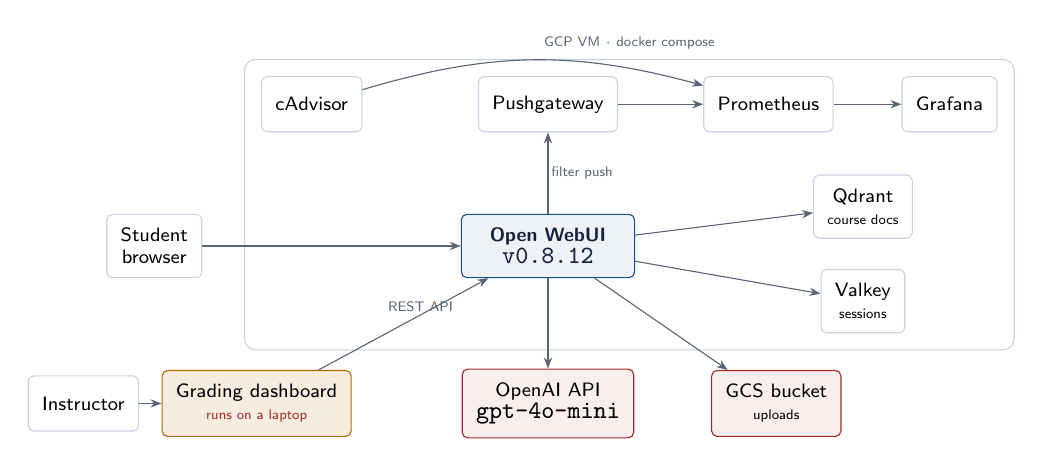
\begin{tikzpicture}[scale=1,every node/.style={transform shape}]
    % --- monitoring band
    \node[box]  at (3.9,4.7) (cad)  {cAdvisor};
    \node[box]  at (6.9,4.7) (pg)   {Pushgateway};
    \node[box]  at (9.7,4.7) (prom) {Prometheus};
    \node[box]  at (12.0,4.7)(graf) {Grafana};
    % --- application band
    \node[box]  at (1.9,2.9) (stu)  {Student\\browser};
    \node[core,minimum width=22mm] at (6.9,2.9) (ow) {Open WebUI\\ \code{v0.8.12}};
    \node[box]  at (10.9,3.4)(qd)   {Qdrant\\ {\tiny course docs}};
    \node[box]  at (10.9,2.2)(rd)   {Valkey\\ {\tiny sessions}};
    % --- external / instructor band
    \node[box,fill=ffcAmber!12,draw=ffcAmber] at (3.2,0.9) (dash)
      {Grading dashboard\\ \textcolor{ffcRed}{\tiny runs on a laptop}};
    \node[box]  at (1.0,0.9) (prof) {Instructor};
    \node[ext]  at (6.9,0.9) (oai)  {OpenAI API\\ \code{gpt-4o-mini}};
    \node[ext]  at (9.8,0.9) (gcs)  {GCS bucket\\ {\tiny uploads}};

    \draw[arr] (stu) -- (ow);
    \draw[arr] (ow) -- (qd);
    \draw[arr] (ow) -- (rd);
    \draw[arr] (ow) -- (oai);
    \draw[arr] (ow) -- (gcs);
    \draw[arr] (ow) -- node[lbl,right]{filter push} (pg);
    \draw[arr] (pg) -- (prom);
    \draw[arr] (cad) to[bend left=16] (prom);   % arc gently over Pushgateway
    \draw[arr] (prom) -- (graf);
    \draw[arr] (prof) -- (dash);
    \draw[arr] (dash) -- node[lbl,above,pos=0.6]{REST API} (ow);
    \begin{scope}[on background layer]
      \node[fit=(cad)(graf)(ow)(qd)(rd)(pg),draw=ffcRule,rounded corners,
            inner sep=6pt,label={[font=\tiny,text=ffcGrey]above:GCP VM $\cdot$ docker compose}] {};
    \end{scope}
  \end{tikzpicture}
  \end{center}
  \vspace{-0.4em}
  {\footnotesize Eight containers on one VM. Retrieval over course documents in Qdrant.
  Chat metrics pushed by a plugin. \bad{The grading dashboard is the outlier --- it is not hosted.}}
  \note{Walk the diagram left to right. Land on the one thing in amber: the professor's tool runs on a laptop. That is workstream A's headline problem.}
\end{frame}

%== 5 =========================================================================
\begin{frame}{The lesson that shaped this project}
  \vspace{-0.3em}
  \begin{columns}[T]
    \begin{column}{0.47\textwidth}
      \textbf{\bad{Before}} --- Spring 2026 and earlier
      \begin{center}
      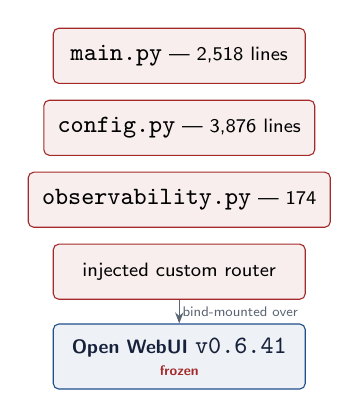
\begin{tikzpicture}
        \node[ext,minimum width=32mm] (a) {\code{main.py} --- 2{,}518 lines};
        \node[ext,minimum width=32mm,below=2mm of a] (b) {\code{config.py} --- 3{,}876 lines};
        \node[ext,minimum width=32mm,below=2mm of b] (c) {\code{observability.py} --- 174};
        \node[ext,minimum width=32mm,below=2mm of c] (d) {injected custom router};
        \node[core,minimum width=32mm,below=3mm of d] (e) {Open WebUI \code{v0.6.41}\\ \textcolor{ffcRed}{\tiny frozen}};
        \draw[arr] (d) -- node[lbl,right]{bind-mounted over} (e);
      \end{tikzpicture}
      \end{center}
      \vspace{2pt}
      {\footnotesize \bad{$\approx$6{,}500 lines} of forked vendor code, re-merged by hand
      on every upgrade. Users reached a feature via a \emph{browser bookmarklet}.}
    \end{column}
    \begin{column}{0.47\textwidth}
      \textbf{\good{After}} --- what we inherited
      \begin{center}
      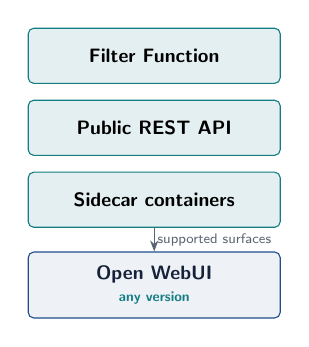
\begin{tikzpicture}
        \node[newb,minimum width=32mm] (f) {Filter Function};
        \node[newb,minimum width=32mm,below=2mm of f] (g) {Public REST API};
        \node[newb,minimum width=32mm,below=2mm of g] (h) {Sidecar containers};
        \node[core,minimum width=32mm,below=3mm of h] (i) {Open WebUI\\ \textcolor{ffcTeal}{\tiny any version}};
        \draw[arr] (h) -- node[lbl,right]{supported surfaces} (i);
      \end{tikzpicture}
      \end{center}
      \vspace{2pt}
      {\footnotesize The \code{Dockerfile} is now \good{one line}. Every customisation
      rides a documented plugin or API surface.}
    \end{column}
  \end{columns}
  \vspace{0.1em}
  \centerline{\small\textit{This is the previous team's real achievement --- and it is why this semester is possible.}}
  \note{Give the last team credit. Six and a half thousand lines of fork to get two features. The bookmarklet detail always lands -- mention it.}
\end{frame}

%== 6 =========================================================================
\begin{frame}{Where it still hurts}
  \vspace{0.2em}
  \begin{center}\footnotesize
  \begin{tabular}{p{5.6cm}p{6.6cm}}
    \toprule
    \textbf{Problem} & \textbf{Consequence} \\
    \midrule
    Pinned to \code{v0.8.12}; upstream ships \code{v0.11.x} & Three minor versions of fixes, features --- and \emph{migrations} --- deferred \\
    Metrics plugin is pasted into the admin UI by hand after every deploy & Deployment is not reproducible; metrics vanish silently \\
    That plugin is synchronous, with blocking network I/O and shared state & On the v0.9+ async core it degrades every concurrent user \\
    \bad{Grading dashboard is not hosted} & A professor needs SSH and a terminal to grade \\
    No CI, no automated smoke test & Past upgrades broke things silently \\
    No alerting on \code{/ready} & An outage was discovered from students \\
    Two RAG stacks, two scoring implementations & Ambiguity about which numbers are canonical \\
    Default \code{admin/admin}; unrotated leaked key & Straightforward security debt \\
    \bottomrule
  \end{tabular}
  \end{center}
  \vspace{0.4em}
  \centerline{\small None of this is exotic. It is the gap between \emph{a system that works} and \emph{a system you can hand over}.}
  \note{Read only three or four rows aloud -- hosted dashboard, no CI, version gap. Close with the "gap between works and handover" line.}
\end{frame}

%== 7 =========================================================================
\sectionslide{Workstream A}{Harden and modernise}{Weeks 1--15 $\cdot$ this must not slip}

%== 8 =========================================================================
\begin{frame}{The compatibility contract}
  \vspace{0.5em}
  \begin{block}{The rule}
    \normalsize Open WebUI is a \hl{dependency}, not a codebase we own. We must be able to
    pull any published release and have the platform work --- with no merge, no patch,
    no re-fork.
  \end{block}
  \vspace{0.6em}
  \begin{columns}[T]
    \begin{column}{0.55\textwidth}
      {\small Every feature must ride a surface that upstream \hl{publishes, documents,
      and versions}.\\[6pt]
      If a feature cannot be built that way, the \emph{feature} is redesigned or dropped.
      The core is never modified.}
    \end{column}
    \begin{column}{0.42\textwidth}
      \begin{block}{The one-sentence test}
        \small \textit{If upstream cut a release tomorrow and we ran it unchanged, would
        this still work?}\\[4pt]
        If the answer needs ``well, as long as they don't change\ldots'', it is forbidden.
      \end{block}
    \end{column}
  \end{columns}
  \note{Slow down here. This is the intellectual core of the deck. The one-sentence test is what they should apply in code review all semester.}
\end{frame}

%== 9 =========================================================================
\begin{frame}{Where we are allowed to build}
  \vspace{0.2em}
  \begin{center}\footnotesize
  \begin{tabular}{llp{6.4cm}}
    \toprule
    & \textbf{Surface} & \textbf{Use it for} \\
    \midrule
    A1 & Environment / admin settings & models, RAG parameters, STT and TTS engines, OTel export \\
    A2 & Filter Functions & observing or lightly rewriting a request in flight \\
    A3 & Pipe Functions & exposing our own logic as a selectable ``model'' \\
    A4 & Action Functions & per-message buttons --- e.g.\ \emph{start a voice session} \\
    A5 & Pipelines server & anything needing its own dependencies, GPU, or heavy compute \\
    A6 & Tools / OpenAPI / MCP & letting the model call our services \\
    A7 & Public REST API & grading extraction, KB sync, \hl{the avatar app} \\
    A8 & Sidecar containers & exporters, our own web applications \\
    A9 & Reverse-proxy composition & TLS, auth, path routing on one hostname \\
    A10 & Knowledge Bases and Skills & course documents and frameworks, professor-editable \\
    \bottomrule
  \end{tabular}
  \end{center}
  \vspace{0.3em}
  \centerline{\small\textbf{Heuristic:} needs to see \emph{inside} a request $\to$ A2--A4. Needs its own runtime $\to$ A5/A8, talking over A7.}
  \note{Do not read the table. Point at A7 and A8 -- those two are what the avatar work will use. The heuristic line is the takeaway.}
\end{frame}

%== 10 ========================================================================
\begin{frame}{What is forbidden --- permanently}
  \vspace{0.3em}
  \begin{center}\footnotesize
  \begin{tabular}{lp{5.9cm}p{5.0cm}}
    \toprule
    & \textbf{Forbidden} & \textbf{Why} \\
    \midrule
    F1 & Mounting or copying anything into \code{/app/backend/open\_webui/} & this \emph{is} the fork \\
    F2 & Adding modules to the \code{open\_webui} package & same, plus coupling to internals \\
    F3 & Building a custom image from modified source & tracks upstream by hand forever \\
    F4 & JavaScript injection into the Svelte frontend & no contract; breaks on any refactor \\
    F5 & Direct SQL against Open WebUI's schema & the schema is private, and \emph{did} change \\
    F6 & Monkeypatching internals from a Function & a fork wearing a plugin costume \\
    F7 & Relying on undocumented endpoints or fields & fine until it isn't; fails silently \\
    F8 & Pinning to an old release to dodge migration work & \bad{this is exactly how v0.6.41 happened} \\
    \bottomrule
  \end{tabular}
  \end{center}
  \vspace{0.4em}
  \centerline{\small It always starts the same way: \textit{``it's just one file, we'll mount it read-only.''}}
  \note{F6 and F8 are the ones teams actually violate. The closing quote is the warning to remember.}
\end{frame}

%== 11 ========================================================================
\begin{frame}{Audit: what we still have to strip out}
  \vspace{0.2em}
  {\footnotesize \good{Good news:} the active stack is already compliant --- no compose file
  mounts anything into Open WebUI's source tree. What remains is peripheral coupling and
  \emph{loaded guns left in the tree.}}
  \vspace{0.5em}
  \begin{center}\footnotesize
  \begin{tabular}{lp{4.8cm}p{5.2cm}l}
    \toprule
    & \textbf{Finding} & \textbf{Action} & \textbf{Risk} \\
    \midrule
    C-1 & the vendor-fork source under \code{legacy/} --- with a README telling you how to re-fork & delete from the tree; leave a tombstone pointing at the commit & \bad{High} \\
    C-2 & \code{--legacy} direct-SQLite flag (a \code{TODO} stub) & delete the flag; REST API is the only path & Med \\
    C-3 & custom \code{build:} context for Open WebUI & replace with a pinned \code{image:}; delete the \code{Dockerfile} & Low \\
    C-4 & metrics filter: sync, blocking I/O, shared state & rewrite async, or retire it for native OTel & \bad{High} \\
    C-6 & \code{:latest} images (Qdrant, cAdvisor) & pin every image & Med \\
    C-7 & Grafana 9.0.0, default \code{admin/admin} & upgrade; remove the default password & \bad{High} \\
    C-8/9 & two RAG stacks, two scoring implementations & pick one canonical each, in writing & Med \\
    C-10 & previously leaked provider key not yet rotated & rotate at the provider; add \code{gitleaks} to CI & \bad{High} \\
    \bottomrule
  \end{tabular}
  \end{center}
  \note{C-1 is the headline: the repo still contains working instructions for re-creating the fork. Deleting it is a five-minute job with outsized value.}
\end{frame}

%== 12 ========================================================================
\begin{frame}{Version debt: what three releases cost us}
  \vspace{0.4em}
  \begin{center}\small
  \begin{tabular}{lp{3.7cm}p{7.0cm}}
    \toprule
    \textbf{Release} & \textbf{Change} & \textbf{What it means for us} \\
    \midrule
    \code{v0.9.0} & backend went \hl{async top to bottom} & \bad{our Filter Function must be migrated} --- sync plugin code with blocking I/O is now actively harmful \\[4pt]
    \code{v0.10.0} & \code{config} table replaced by a per-key table & \bad{one-way migration.} An older instance pointed at a migrated database fails immediately \\[4pt]
    \code{v0.11.0} & additive columns only; \code{psycopg} v3; major UI reorganisation & low migration risk, \hl{high documentation risk} --- every screenshot and click-path we publish is now wrong \\
    \bottomrule
  \end{tabular}
  \end{center}
  \vspace{0.7em}
  \centerline{\small We are on \code{v0.8.12}. \textbf{The longer this waits, the more expensive it gets ---}}
  \centerline{\small\textit{which is precisely the dynamic that produced the v0.6.41 freeze.}}
  \note{The point is not "upgrades are nice". It is that deferred migrations compound, and this project already has the scar to prove it.}
\end{frame}

%== 13 ========================================================================
\begin{frame}{How we will do the upgrade}
  \vspace{0.4em}
  \begin{columns}[T]
    \begin{column}{0.56\textwidth}
      \small
      \begin{enumerate}
        \item Snapshot production --- and \hl{restore the snapshot into the test stack}.
              \textit{A backup you have never restored is not a backup.}
        \item Upgrade the test stack first, on real production data.
        \item Move \hl{one minor version at a time}: 0.8 $\to$ 0.9 $\to$ 0.10 $\to$ 0.11.
              Migrations run sequentially; a single jump makes failures unattributable.
        \item Run the smoke suite at every step. Write the runbook \emph{as you go}.
        \item Decide \hl{SQLite $\to$ PostgreSQL} explicitly, and record the decision either way.
        \item Schedule the production window with the rollback written \emph{before} you start.
        \item Re-shoot every screenshot for the new UI.
      \end{enumerate}
    \end{column}
    \begin{column}{0.40\textwidth}
      \begin{block}{Done when}
        \small
        Production runs the current release.\\[3pt]
        The runbook exists \emph{and was followed}.\\[3pt]
        The smoke suite passes.\\[3pt]
        Docs match what a user actually sees.\\[3pt]
        The rollback is \hl{proven}, not theorised.
      \end{block}
      \vspace{0.4em}
      {\footnotesize \bad{Schedule this outside student deadline weeks.}}
    \end{column}
  \end{columns}
  \note{Step 1 and step 6 are the professional habits worth arguing for. Most teams skip both and get away with it until they don't.}
\end{frame}

%== 14 ========================================================================
\begin{frame}{CI/CD --- and the guard that keeps the fork dead}
  \vspace{0.3em}
  \begin{columns}[T]
    \begin{column}{0.52\textwidth}
      \textbf{\color{ffcBlue}Pipeline, by value per hour spent}
      \begin{enumerate}\small
        \item \textbf{Smoke test on every push} --- bring the stack up, wait for
              \code{/health} then \code{/ready}, send a chat completion, upload a
              document, assert retrieval returns it
        \item \textbf{Fork guard} (below)
        \item \textbf{Secret scanning} --- \code{gitleaks}, including history
        \item \textbf{Lint and unit tests} --- especially on the scoring service:
              \emph{it produces numbers that become grades}
        \item \textbf{Deploy on tag} --- pull, restart, re-smoke, auto-rollback
      \end{enumerate}
    \end{column}
    \begin{column}{0.45\textwidth}
      \begin{block}{The fork guard --- fails the build when\ldots}
        \small
        a compose file mounts into \code{open\_webui/}\\[2pt]
        the image is built from modified source\\[2pt]
        Python opens SQLite against Open WebUI's data\\[2pt]
        \code{gitleaks} finds a credential\\[2pt]
        any image reference ends in \code{:latest}
      \end{block}
      \vspace{0.3em}
      {\footnotesize $\approx$40 lines of grep and one GitHub Action. \hl{This is what makes
      the policy real instead of aspirational.} Build it in Week 2.}
    \end{column}
  \end{columns}
  \note{Emphasise: a policy nobody enforces is a wish. Forty lines of grep converts a document into a constraint.}
\end{frame}

%== 15 ========================================================================
\begin{frame}{Two fixes that change who can use this}
  \vspace{0.4em}
  \begin{columns}[T]
    \begin{column}{0.47\textwidth}
      \textbf{\color{ffcBlue}Host the grading dashboard}\\[4pt]
      {\small Today a professor must SSH into a GCP VM and run a shell script.\\[5pt]
      Containerise the backend, build the frontend to static assets, put Nginx in front with
      TLS and real authentication, and give them a \hl{URL}.\\[5pt]
      \textit{Watch:} make \code{/refresh} asynchronous with visible progress --- it scores
      every question through a paid API.}
      \\[6pt]
      {\footnotesize\good{Done when} a professor grades with no terminal, no VPN, and no help
      from a student.}
    \end{column}
    \begin{column}{0.47\textwidth}
      \textbf{\color{ffcBlue}Observability without manual steps}\\[4pt]
      {\small Chat metrics currently depend on a human pasting Python into an admin form
      after every deployment.\\[5pt]
      Fix the \emph{class} of problem: enable Open WebUI's \hl{native OpenTelemetry export}
      into a collector, and scrape that. Then retire the filter --- or rewrite it async.\\[5pt]
      Add a \code{/ready} uptime check that alerts \emph{a person}, and a memory alert as a
      leading indicator.}
      \\[6pt]
      {\footnotesize\good{Done when} a clean deployment produces metrics with zero manual
      steps, and an induced outage pages someone in five minutes.}
    \end{column}
  \end{columns}
  \note{These two are the highest-adoption-value items in the whole plan. The dashboard one is the difference between a tool that gets used and one that doesn't.}
\end{frame}

%== 16 ========================================================================
\begin{frame}{Remove the ambiguity}
  \vspace{0.5em}
  \begin{columns}[T]
    \begin{column}{0.31\textwidth}
      \begin{block}{Scoring exists twice}
        \small JavaScript and Python, kept in sync by hand.\\[4pt]
        Declare \hl{Python canonical}. Retire the prototype. Add tests that pin the rubric
        arithmetic and ABI weights.
      \end{block}
    \end{column}
    \begin{column}{0.31\textwidth}
      \begin{block}{RAG exists twice}
        \small Native Qdrant (what students use) and a standalone ChromaDB pipeline
        (which nothing uses).\\[4pt]
        Retire it, or promote it behind a \hl{Pipelines server}. Decide in writing.
      \end{block}
    \end{column}
    \begin{column}{0.31\textwidth}
      \begin{block}{Extraction is heuristic}
        \small Student questions are found by punctuation and keywords.\\[4pt]
        \hl{Measure its accuracy} against a hand-labelled sample before trusting the scores
        built on top of it.
      \end{block}
    \end{column}
  \end{columns}
  \vspace{0.9em}
  \centerline{\small Each of these will eventually produce a wrong answer that nobody can explain.}
  \centerline{\small\textit{Dead code with live bugs is a tax --- the citation bug we fixed lived in the stack nobody runs.}}
  \note{The third column is the sleeper. If question extraction is 70 percent accurate, every grade downstream inherits that error, silently.}
\end{frame}

%== 17 ========================================================================
\sectionslide{Workstream B}{Embodied advising}{The new research track $\cdot$ Weeks 3--15}

%== 18 ========================================================================
\begin{frame}{Why typing is not enough}
  \vspace{0.2em}
  \begin{columns}[T]
    \begin{column}{0.5\textwidth}
      {\small FIN 602 exists to prepare students for \hl{a room with a real family in it}.
      \\[8pt]
      That room demands: listening while someone is still talking, hearing hesitation,
      holding eye contact through an uncomfortable question about money, and asking the
      follow-up \emph{out loud} --- without a backspace key.}
    \end{column}
    \begin{column}{0.46\textwidth}
      \begin{block}{The gap}
        \small The platform teaches the \emph{content} of good advising well.\\[4pt]
        It cannot teach the \emph{performance} of it --- because typing removes every one of
        those pressures.\\[4pt]
        A student can draft, delete, and reword for ninety seconds before asking
        \textit{``what happens to the business if something happens to you?''}
      \end{block}
    \end{column}
  \end{columns}
  \vspace{0.8em}
  \begin{block}{This semester's hypothesis --- and it is a hypothesis}
    \small A spoken, face-to-face AI client produces meaningfully better preparation than a
    text chatbot --- and we can \hl{measure whether that is true} with the scoring pipeline
    the platform already has. This track is designed to be allowed to answer \emph{no}.
  \end{block}
  \note{This is the emotional centre of the pitch. Deliver the backspace-key line slowly. Then immediately frame it as testable, not assumed.}
\end{frame}

%== 19 ========================================================================
\begin{frame}{What we are actually building}
  \vspace{0.5em}
  {\small A student opens a link, sees a face, and says out loud:}
  \vspace{0.3em}
  \begin{center}
    \colorbox{ffcMist}{\parbox{0.8\textwidth}{\vspace{3pt}\small\itshape\centering
    ``Hi --- I'm going to ask you a few questions about your family's finances.
    Is that alright?''\vspace{3pt}}}
  \end{center}
  \vspace{0.3em}
  {\small The client on screen \hl{looks at them, nods, and answers in their own voice},
  in character, with their own financial situation --- drawn from the same course documents
  the text bot already uses.\\[4pt]
  If the student interrupts, the client \hl{stops talking}. If the student goes quiet, the
  client waits --- and may eventually prompt them, the way a real, slightly impatient client
  would.\\[4pt]
  At the end, the transcript lands in \hl{the same grading dashboard}, scored on the same
  seven dimensions and the same ABI rubric.}
  \vspace{0.5em}
  \begin{block}{What we are \emph{not} building}
    \small A photorealistic digital human. A likeness of any real person. A replacement for
    the text interface --- text stays. Voice and face are an \emph{additional mode}.
  \end{block}
  \note{Read the quoted line as if speaking to the avatar. The "stops talking" detail is what separates a real prototype from a demo video.}
\end{frame}

%== 20 ========================================================================
\begin{frame}{The constraint dictates the architecture}
  \vspace{0.5em}
  {\small The instinct is to put the avatar \emph{inside} the Open WebUI chat window.}
  \vspace{0.4em}
  \begin{block}{That is forbidden --- F3 and F4 at once}
    \small Open WebUI's frontend is a Svelte application we do not own. Embedding a WebRTC
    video pane in it means forking and re-merging that frontend forever ---
    \bad{precisely the mistake this project spent a semester undoing.}
  \end{block}
  \vspace{0.5em}
  {\small So the constraint decides the design, and the design it produces is \good{better}:}
  \vspace{0.3em}
  \centerline{\small\textbf{The avatar is a companion web application in its own container.}}
  \centerline{\small Open WebUI stays the \hl{brain} (model, RAG, knowledge) and the
  \hl{system of record} (transcripts). We talk to it over the public API.}
  \vspace{0.6em}
  \begin{columns}[T]
    \begin{column}{0.49\textwidth}
      {\footnotesize \good{$\rightarrow$} deploy, roll back, and load-test independently\\
      \good{$\rightarrow$} survives every upstream release by construction}
    \end{column}
    \begin{column}{0.49\textwidth}
      {\footnotesize \good{$\rightarrow$} if we kill the track in December, we delete one container\\
      \good{$\rightarrow$} students and professors keep the interface they know}
    \end{column}
  \end{columns}
  \note{This slide is the argument that the compatibility policy is not bureaucracy -- it produced a better architecture than the instinctive one.}
\end{frame}

%== 21 ========================================================================
\begin{frame}{Reference architecture}
  \vspace{-0.3em}
  \begin{center}
  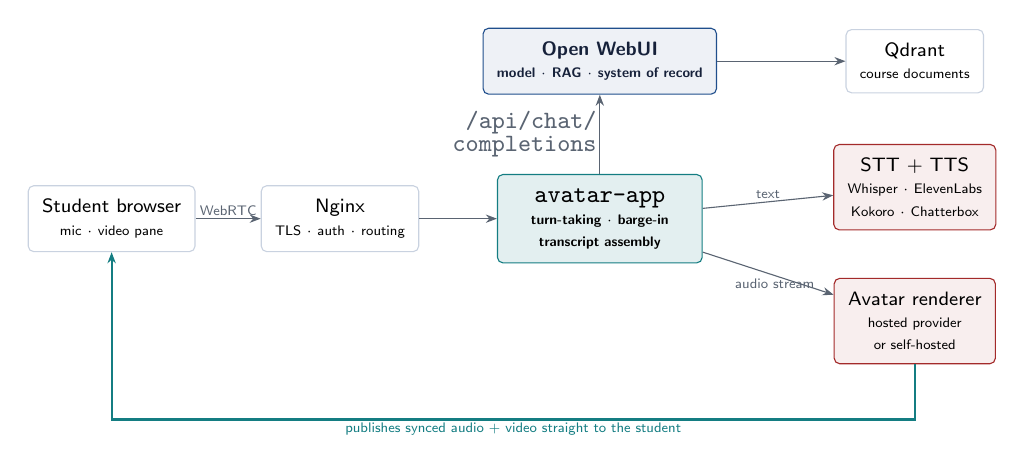
\begin{tikzpicture}[scale=1,every node/.style={transform shape}]
    \node[box]  at (1.7,3.0) (br)  {Student browser\\ {\tiny mic $\cdot$ video pane}};
    \node[box]  at (4.6,3.0) (px)  {Nginx\\ {\tiny TLS $\cdot$ auth $\cdot$ routing}};
    \node[newb,minimum width=26mm] at (7.9,3.0) (app)
        {\code{avatar-app}\\ {\tiny turn-taking $\cdot$ barge-in}\\ {\tiny transcript assembly}};
    \node[core,minimum width=26mm] at (7.9,5.0) (ow)
        {Open WebUI\\ {\tiny model $\cdot$ RAG $\cdot$ system of record}};
    \node[box]  at (11.9,5.0) (qd) {Qdrant\\ {\tiny course documents}};
    \node[ext]  at (11.9,3.4) (stt) {STT + TTS\\ {\tiny Whisper $\cdot$ ElevenLabs}\\ {\tiny Kokoro $\cdot$ Chatterbox}};
    \node[ext]  at (11.9,1.7) (av)  {Avatar renderer\\ {\tiny hosted provider}\\ {\tiny or self-hosted}};

    \draw[arr] (br) -- node[lbl,above]{WebRTC} (px);
    \draw[arr] (px) -- (app);
    \draw[arr] (app) -- node[lbl,left,align=right]{\code{/api/chat/}\\ \code{completions}} (ow);
    \draw[arr] (ow) -- (qd);
    \draw[arr] (app) -- node[lbl,above]{text} (stt);
    \draw[arr] (app) -- node[lbl,below,pos=0.55]{audio stream} (av);
    \draw[arr,draw=ffcTeal,thick] (av.south) -- ++(0,-0.7)
        -| node[lbl,below,pos=0.25,text=ffcTeal]
        {publishes synced audio + video straight to the student} (br.south);
  \end{tikzpicture}
  \end{center}
  \vspace{-0.2em}
  {\footnotesize \good{The pattern that matters:} the renderer is not a step we wait on. It
  \hl{joins the session as its own participant} --- we stream it audio, and it publishes
  finished, lip-synced video directly to the student. That removes a full round trip through
  our server. It is the difference between a video call and a laggy video attachment.}
  \note{Trace the teal arrow. Do not hand-roll WebRTC and turn-taking -- use LiveKit Agents or Pipecat. That is not the semester's research question.}
\end{frame}

%== 22 ========================================================================
\begin{frame}{Latency is the number that decides everything}
  \vspace{0.3em}
  \begin{columns}[T]
    \begin{column}{0.55\textwidth}
      \centering\footnotesize
      \begin{tabular}{lr}
        \toprule
        \textbf{Stage} & \textbf{Realistic} \\
        \midrule
        Voice activity detection / endpointing & 150--300\,ms \\
        Speech to text & 150--300\,ms \\
        \textcolor{ffcRed}{Retrieval (RAG)} & \textcolor{ffcRed}{100--300\,ms} \\
        LLM time-to-first-token & 300--600\,ms \\
        Text to speech, first byte & 150--300\,ms \\
        Avatar render + network & 200--500\,ms \\
        \midrule
        \textbf{First audible syllable} & \textbf{1.0--2.3\,s} \\
        \bottomrule
      \end{tabular}
    \end{column}
    \begin{column}{0.42\textwidth}
      \begin{block}{Targets for this semester}
        \small p50 under \hl{1.2\,s}\\
        p95 under \hl{2.0\,s}\\
        barge-in interrupts within \hl{300\,ms}
      \end{block}
      \vspace{0.3em}
      {\footnotesize Conversation tolerates about a second. Past two, a person stops feeling
      \emph{heard} and starts feeling \emph{processed}.}
    \end{column}
  \end{columns}
  \vspace{0.5em}
  {\footnotesize \bad{The RAG trap:} the text platform retrieves on every turn. In a spoken
  loop that sits directly in the critical path. Strongly consider loading the family scenario
  into the system prompt \emph{once} at session start --- a 2{,}000-token persona brief costs
  less latency than a vector search per turn, every turn.\\[3pt]
  \hl{Instrument every stage separately, in Week 5.} One end-to-end number tells you it is
  slow, not what to fix.}
  \note{The RAG trap is the most useful engineering insight on this slide -- it is counterintuitive and it is where a naive implementation loses half a second per turn.}
\end{frame}

%== 23 ========================================================================
\begin{frame}{Three strategies --- and the one we start with}
  \vspace{0.3em}
  \begin{columns}[T]
    \begin{column}{0.31\textwidth}
      \begin{block}{1. Hosted streaming}
        \footnotesize HeyGen LiveAvatar, Tavus (Phoenix-4), Simli, Anam, bitHuman, Beyond
        Presence, D-ID.\\[4pt]
        Plug into LiveKit or Pipecat; swap providers behind one interface.\\[4pt]
        \textbf{Vendor latency claims are measured under vendor conditions.}
        \hl{Measuring ours is the assignment.}
      \end{block}
    \end{column}
    \begin{column}{0.31\textwidth}
      \begin{block}{2. Self-hosted open source}
        \footnotesize Whisper $\to$ open TTS $\to$ an open lip-sync renderer.\\[4pt]
        \good{For:} no per-minute cost, no student audio leaving our infrastructure.\\[4pt]
        \bad{Against:} needs a GPU we do not have; quality and latency lag; it becomes an
        infrastructure project.
      \end{block}
    \end{column}
    \begin{column}{0.31\textwidth}
      \begin{block}{3. Voice only --- no face}
        \footnotesize Open WebUI \emph{already has} hands-free call mode. STT and TTS are
        configuration, not engineering.\\[4pt]
        Captures much of the benefit --- speaking aloud, no backspace, real-time pressure ---
        at \hl{near-zero build cost}.
      \end{block}
    \end{column}
  \end{columns}
  \vspace{0.7em}
  \begin{block}{Start with \#3, in Week 3}
    \small It de-risks the entire track. If avatars prove too slow, too costly, or too
    fragile, \hl{the course still gains spoken practice this semester.} B0 ships regardless.
  \end{block}
  \note{The strategic point: build the fallback first, and build it in three weeks. That is how you make an ambitious research track safe to attempt.}
\end{frame}

%== 24 ========================================================================
\begin{frame}{What it costs --- and how we stop it running away}
  \vspace{0.4em}
  \begin{columns}[T]
    \begin{column}{0.52\textwidth}
      \centering\footnotesize
      40 students $\times$ 4 sessions $\times$ 15 min $=$ \textbf{40 hours / semester}
      \vspace{0.4em}
      \begin{tabular}{lr}
        \toprule
        \textbf{Line item} & \textbf{Semester} \\
        \midrule
        Avatar streaming ($\sim$\$0.10--0.20/min) & \$240--480 \\
        Speech to text & \$10--30 \\
        Text to speech & \$20--60 \\
        LLM (short spoken turns) & \$15--40 \\
        \midrule
        \textbf{Total} & \textbf{$\approx$\$285--610} \\
        \bottomrule
      \end{tabular}
      \vspace{0.3em}
      {\tiny Checked August 2026. Prices move quarterly --- re-derive at signup and record the date.}
    \end{column}
    \begin{column}{0.45\textwidth}
      \begin{block}{Controls from day one --- not after the first bill}
        \small
        15-minute hard cap, enforced server-side\\[3pt]
        per-student session quota\\[3pt]
        billing alert at 50\% of budget\\[3pt]
        sessions terminate on disconnect\\[3pt]
        a kill switch that needs no redeploy
      \end{block}
      \vspace{0.3em}
      {\footnotesize \bad{Do the arithmetic before advocating self-hosting:} an L4-class GPU
      VM is roughly \$500/month if left running. At 40 hours a semester, \hl{buying beats
      building.} Self-hosting wins on privacy and at scale --- not on cost, here.}
    \end{column}
  \end{columns}
  \note{The self-hosting arithmetic is the slide's punchline. Students instinctively assume open source is cheaper; at this volume it is roughly ten times more expensive.}
\end{frame}

%== 25 ========================================================================
\begin{frame}{How we will evaluate it honestly}
  \vspace{0.3em}
  {\small \good{We already own the outcome measure} --- so use it. Within-subjects,
  counterbalanced: each student practises in two or three modalities with matched scenarios,
  in varied order.}
  \vspace{0.5em}
  \begin{center}\footnotesize
  \begin{tabular}{lp{6.6cm}}
    \toprule
    \textbf{Measure} & \textbf{Question it answers} \\
    \midrule
    7-dimension question quality & do students ask \emph{better} questions when speaking? \\
    ABI trust scores & does modality change how the interaction reads? \\
    Questions asked; session duration & does speaking increase or suppress engagement? \\
    \textcolor{ffcTeal}{Interruptions; talk-time ratio} & \textcolor{ffcTeal}{are students learning to \emph{listen}?} \\
    Hesitation before sensitive questions & does rehearsal reduce discomfort over sessions? \\
    Realism, social presence, anxiety (survey) & is it believable and productive --- or uncanny? \\
    \bottomrule
  \end{tabular}
  \end{center}
  \vspace{0.5em}
  {\footnotesize \bad{Do not over-claim.} The sample is small and the semester is short.
  \textit{``Twelve students, counterbalanced, with these effect sizes and confidence
  intervals''} is a credible result. \textit{``Avatars improve learning''} is not.
  \hl{A well-designed study with an honest negative result is the better deliverable} --- and
  it will be graded that way.}
  \note{The teal row is the genuinely novel contribution: whether a student lets the client finish talking may be a better measure of advising skill than anything the current rubric captures.}
\end{frame}

%== 26 ========================================================================
\begin{frame}{Phases and gates}
  \vspace{0.1em}
  \begin{center}\small
  \begin{tabular}{llp{6.0cm}p{3.6cm}}
    \toprule
    & \textbf{Weeks} & \textbf{Deliverable} & \textbf{Gate} \\
    \midrule
    \textbf{B0} & 3--5 & hands-free spoken practice on Open WebUI's own call mode & \emph{ships regardless} \\[3pt]
    \textbf{B1} & 4--7 & two providers behind one interface, measured on latency, cost, barge-in & \hl{choose --- or recommend stopping} \\[3pt]
    \textbf{B2} & 7--12 & \code{avatar-app} container; transcripts written back into grading & \hl{five students complete a full session} \\[3pt]
    \textbf{B3} & 11--15 & text vs voice vs avatar, measured on the existing rubric & \hl{evidence-backed go / no-go} \\
    \bottomrule
  \end{tabular}
  \end{center}
  \vspace{0.3em}
  \begin{block}{The gates are real}
    \small ``Stop'' is an acceptable outcome at every gate. \bad{``We didn't measure'' is not.}\\[4pt]
    And build the transcript write-back \emph{first} in B2, not last --- an avatar session that
    never reaches the grading dashboard is a demo, not a feature.
  \end{block}
  \note{Make the kill switch explicit and unembarrassing. Research tracks that cannot fail are not research tracks.}
\end{frame}

%== 27 ========================================================================
\begin{frame}{Ethics, privacy, and consent --- settle this in Week 2}
  \vspace{0.4em}
  \begin{columns}[T]
    \begin{column}{0.48\textwidth}
      \small
      \begin{itemize}
        \item Student transcripts are \hl{education records} under FERPA. Adding audio adds a
              biometric-adjacent identifier to that.
        \item \hl{Written informed consent} before any recording: what is captured, where it
              lives, how long, who sees it, how to opt out --- \textbf{without affecting a grade}.
        \item \bad{No likeness of any real person.} Use provider stock avatars under licence.
              Do not clone a professor's face or voice ``as a joke.''
      \end{itemize}
    \end{column}
    \begin{column}{0.48\textwidth}
      \small
      \begin{itemize}
        \item \hl{Disclose the AI.} We are teaching advising, not testing whether students can
              be fooled.
        \item \hl{Minimise data.} Prefer keeping the transcript and discarding the audio.
        \item \hl{Read the vendor's terms} before sending one student's voice: retention,
              training use, sub-processors, region. For an education platform this can
              outweigh a latency win.
        \item Ask about \hl{IRB review} in Week 2 --- approval takes longer than you think.
      \end{itemize}
    \end{column}
  \end{columns}
  \vspace{0.5em}
  \centerline{\small\textit{Settle these before the data exists --- not in Week 13, when it already does.}}
  \note{Do not rush this slide. For a university deployment it is the one that determines whether the project is allowed to run at all.}
\end{frame}

%== 28 ========================================================================
\sectionslide{Execution}{Timeline, roles, and risk}{How the two tracks stay in balance}

%== 29 ========================================================================
\begin{frame}{The semester}
  \vspace{0.2em}
  \begin{center}\scriptsize
  \begin{tabular}{clp{4.9cm}p{4.9cm}}
    \toprule
    \textbf{Wk} & \textbf{Starts} & \textbf{Workstream A --- platform} & \textbf{Workstream B --- avatars} \\
    \midrule
    1 & Aug 24 & set up; run the stack; read the handoff & scope the landscape \\
    2 & Aug 31 & \hl{CI skeleton + fork guard + gitleaks} & requirements; \bad{consent and IRB questions} \\
    3 & Sep 7 & snapshot production; restore into test & \hl{B0: voice session end to end} \\
    4 & Sep 14 & test stack to v0.9.x; migrate the filter & provider shortlist; cost model \\
    5 & Sep 21 & v0.10.x on test & \hl{B0 demo}; latency baseline measured \\
    6 & Sep 28 & v0.11.x on test; docs re-shot & provider \#1 in a bare harness \\
    7 & Oct 5 & \hl{production upgrade window} & provider \#2; head-to-head \\
    8 & Oct 12 & hosted dashboard: container, proxy, TLS & \hl{Gate 1 --- pick, or stop} \\
    9 & Oct 19 & dashboard auth; professor walkthrough & companion app skeleton \\
    10 & Oct 26 & OTel + alerting live & avatar joins the session; barge-in works \\
    11 & Nov 2 & scoring consolidation + tests & transcript write-back \\
    12 & Nov 9 & RAG decision executed & \hl{Gate 2 --- five real sessions} \\
    13 & Nov 16 & performance and cost review & evaluation sessions run \\
    14 & Nov 23 & \textit{(short week)} runbooks and documentation & data analysed \\
    15 & Nov 30 & freeze; handoff written & recommendation drafted \\
    16 & Dec 7 & \multicolumn{2}{l}{\hl{final presentation and handoff}} \\
    \bottomrule
  \end{tabular}
  \end{center}
  \note{Point at weeks 2, 7, and 8. A and B are deliberately interleaved so neither starves. The upgrade lands before the avatar work gets heavy.}
\end{frame}

%== 30 ========================================================================
\begin{frame}{Who owns what}
  \vspace{0.5em}
  \begin{center}\small
  \begin{tabular}{lp{6.9cm}c}
    \toprule
    \textbf{Role} & \textbf{Owns} & \textbf{Track} \\
    \midrule
    Platform / DevOps lead & compose stack, upgrade path, CI/CD, proxy, secrets, backups & A \\
    Backend / integrations & grading service, extraction, scoring, Pipelines & A \\
    Realtime / avatar engineer & STT $\to$ LLM $\to$ TTS $\to$ avatar, latency, provider SDKs & B \\
    Frontend / UX & hosted dashboard, avatar app, session flow & A + B \\
    Data / assessment & evaluation design, metrics, transcript merge, outcomes & A + B \\
    \bottomrule
  \end{tabular}
  \end{center}
  \vspace{0.8em}
  \begin{block}{One duty every member carries}
    \small Review every pull request against the compatibility policy. The question is fixed:\\
    \centerline{\textit{``Which extension surface --- and what happens on the next upstream release?''}}
  \end{block}
  \vspace{0.3em}
  {\footnotesize On a smaller team one person holds two roles. \hl{The roles still exist, and so does the accountability.}}
  \note{Roles are about accountability, not headcount. The shared review duty is what keeps the policy alive when the deadline pressure arrives.}
\end{frame}

%== 31 ========================================================================
\begin{frame}{What could go wrong}
  \vspace{0.2em}
  \begin{center}\footnotesize
  \begin{tabular}{p{5.4cm}cp{5.6cm}}
    \toprule
    \textbf{Risk} & \textbf{Sev} & \textbf{Mitigation} \\
    \midrule
    The v0.10 config migration corrupts production data & \bad{High} & rehearse on a restored snapshot; verify the restore \emph{first}; run outside deadline weeks \\
    \bad{The avatar absorbs the semester and the platform work slips} & \bad{High} & A1 and A2 land before Week 8 --- the timeline front-loads them deliberately \\
    Avatar latency lands at 3+ seconds & Med & measure in Week 5; B0 voice-only ships regardless \\
    Streaming costs surprise the department & Med & caps, quotas, and a billing alarm from day one \\
    Voice and video create privacy exposure & \bad{High} & consent, no real likenesses, documented retention, sign-off \\
    A provider reprices or deprecates mid-semester & Med & provider-agnostic interface; keep the runner-up warm \\
    Somebody proposes embedding video in the chat page & Med & \bad{policy F3/F4 --- refuse.} The companion app exists for this reason \\
    Knowledge is lost at handoff, again & Med & \code{HANDOFF.md} updated continuously, not written in Week 15 \\
    \bottomrule
  \end{tabular}
  \end{center}
  \note{Row two is the one to dwell on. The exciting track will try to eat the boring track, and the boring track is what the course actually depends on.}
\end{frame}

%== 32 ========================================================================
\begin{frame}{Done means done}
  \vspace{0.5em}
  {\small The semester is complete when \hl{all eight} are true:}
  \vspace{0.4em}
  \begin{columns}[T]
    \begin{column}{0.48\textwidth}
      \small
      \begin{enumerate}
        \item Production runs a current release, upgraded via a written, \emph{rehearsed} runbook.
        \item A push runs CI; a tag deploys; a red build blocks the merge.
        \item The fork guard exists and passes --- and no re-forking instructions remain in the tree.
        \item A professor grades from an authenticated URL, with no terminal.
      \end{enumerate}
    \end{column}
    \begin{column}{0.48\textwidth}
      \small
      \begin{enumerate}
        \setcounter{enumi}{4}
        \item Metrics and alerting work from a clean deployment, with zero manual steps.
        \item Scoring and retrieval each have one canonical implementation, with tests.
        \item A working avatar prototype exists, real students used it, and a written
              evaluation backs a go/no-go call.
        \item \code{HANDOFF.md} lets the next team start in Week 1 --- not Week 4.
      \end{enumerate}
    \end{column}
  \end{columns}
  \note{Read these as acceptance criteria, not aspirations. Every one is verifiable by someone who was not in the room.}
\end{frame}

%== 33 ========================================================================
\begin{frame}[plain]
  \begin{tikzpicture}[remember picture,overlay]
    \fill[ffcInk] (current page.south west) rectangle (current page.north east);
    \node[anchor=west,text width=0.82\paperwidth] at ([xshift=1.2cm,yshift=1.5cm]current page.west)
      {\color{white}\LARGE\bfseries The goal is not to finish\\[6pt] FamilyFinanceChat.};
    \node[anchor=west,text width=0.78\paperwidth] at ([xshift=1.2cm,yshift=-0.5cm]current page.west)
      {\color{ffcRule}\large It is to leave a system where the interesting work is
       \textbf{\color{white}the pedagogy}, not \textbf{\color{white}the plumbing}.};
    \node[anchor=west,text width=0.78\paperwidth] at ([xshift=1.2cm,yshift=-2.3cm]current page.west)
      {\color{ffcGrey}\small Every hour spent this semester on upgrades, CI, and hosting is an
       hour a future team does not spend re-learning why the fork was a mistake.};
    \node[anchor=south east] at ([xshift=-1.2cm,yshift=0.9cm]current page.south east)
      {\color{ffcTeal}\small\bfseries Questions?};
  \end{tikzpicture}
  \note{Close on purpose, not on tasks. Then open the floor -- expect questions on avatar cost, on privacy, and on whether the upgrade can wait. It cannot.}
\end{frame}

\end{document}
"
% (build.sh does this for you and names the output ...-notes.pdf)
\ifdefined\SHOWNOTES\setbeameroption{show notes}\fi

\usepackage[T1]{fontenc}
\usepackage[utf8]{inputenc}
\usepackage{helvet}
\renewcommand{\familydefault}{\sfdefault}
\usepackage{microtype}
\usepackage{booktabs}
\usepackage{tikz}
\usepackage{xcolor}
\usetikzlibrary{arrows.meta,positioning,fit,backgrounds,shapes.geometric}

%------------------------------------------------------------------ palette --
\definecolor{ffcInk}{HTML}{16213A}
\definecolor{ffcBlue}{HTML}{1F4E8C}
\definecolor{ffcTeal}{HTML}{147D82}
\definecolor{ffcAmber}{HTML}{B26A00}
\definecolor{ffcRed}{HTML}{A32A2A}
\definecolor{ffcGrey}{HTML}{5A6472}
\definecolor{ffcMist}{HTML}{EEF1F6}
\definecolor{ffcRule}{HTML}{C9D2E0}

%--------------------------------------------------------------------- theme --
\usetheme{default}
\usecolortheme{default}
\setbeamercolor{normal text}{fg=ffcInk}
\setbeamercolor{structure}{fg=ffcBlue}
\setbeamercolor{frametitle}{fg=white,bg=ffcInk}
\setbeamercolor{title}{fg=white}
\setbeamercolor{alerted text}{fg=ffcRed}
\setbeamercolor{block title}{fg=white,bg=ffcBlue}
\setbeamercolor{block body}{fg=ffcInk,bg=ffcMist}
\setbeamerfont{frametitle}{series=\bfseries,size=\large}
\setbeamerfont{title}{series=\bfseries,size=\LARGE}
\setbeamertemplate{navigation symbols}{}
\setbeamertemplate{itemize item}{\color{ffcBlue}\rule[0.35ex]{0.55ex}{0.55ex}}
\setbeamertemplate{itemize subitem}{\color{ffcTeal}\rule[0.35ex]{0.4ex}{0.4ex}}
\setbeamertemplate{section in toc}{\color{ffcInk}\inserttocsectionnumber.~\inserttocsection}

\setbeamertemplate{frametitle}{%
  \nointerlineskip
  \begin{beamercolorbox}[wd=\paperwidth,ht=3.1ex,dp=1.5ex,leftskip=0.9em,rightskip=0.9em]{frametitle}
    \usebeamerfont{frametitle}\insertframetitle%
    \hfill\raisebox{0.2ex}{\scriptsize\color{ffcRule}\insertframenumber}
  \end{beamercolorbox}%
  \vskip0.6ex
}
\setbeamertemplate{footline}{%
  \hbox{\begin{beamercolorbox}[wd=\paperwidth,ht=2.2ex,dp=1ex,leftskip=0.9em,rightskip=0.9em]{}
    {\tiny\color{ffcGrey}FamilyFinanceChat \quad$\cdot$\quad Fall 2026 Project Kickoff}
  \end{beamercolorbox}}
}

%----------------------------------------------------------------- shortcuts --
\newcommand{\hl}[1]{\textcolor{ffcBlue}{\textbf{#1}}}
\newcommand{\bad}[1]{\textcolor{ffcRed}{\textbf{#1}}}
\newcommand{\good}[1]{\textcolor{ffcTeal}{\textbf{#1}}}
\newcommand{\code}[1]{{\small\texttt{#1}}}
% Centred text that WRAPS (plain TeX \centerline does not, and runs off the slide).
\renewcommand{\centerline}[1]{{\par\centering #1\par}}
\newcommand{\yes}{\textcolor{ffcTeal}{\textbf{\checkmark}}}
\newcommand{\no}{\textcolor{ffcRed}{\textbf{\texttimes}}}

% Section divider
\newcommand{\sectionslide}[3]{%
  \begin{frame}[plain]
    \begin{tikzpicture}[remember picture,overlay]
      \fill[ffcInk] (current page.south west) rectangle (current page.north east);
      \node[anchor=west,text width=0.8\paperwidth] at ([xshift=1.2cm,yshift=0.7cm]current page.west)
        {\color{white}\Huge\bfseries #1};
      \node[anchor=west,text width=0.8\paperwidth] at ([xshift=1.2cm,yshift=-0.6cm]current page.west)
        {\color{ffcRule}\large #2};
      \node[anchor=west] at ([xshift=1.2cm,yshift=-1.9cm]current page.west)
        {\color{ffcTeal}\small\bfseries #3};
    \end{tikzpicture}
  \end{frame}
}

% tikz node styles
\tikzset{
  box/.style={rounded corners=2pt,draw=ffcRule,fill=white,inner sep=5pt,
              align=center,font=\scriptsize,minimum height=7mm},
  core/.style={box,fill=ffcMist,draw=ffcBlue,text=ffcInk,font=\scriptsize\bfseries},
  newb/.style={box,fill=ffcTeal!12,draw=ffcTeal,font=\scriptsize\bfseries},
  ext/.style={box,fill=ffcRed!8,draw=ffcRed,font=\scriptsize},
  arr/.style={-{Stealth[length=4pt]},draw=ffcGrey,thin},
  lbl/.style={font=\tiny,text=ffcGrey,inner sep=1pt},
}

%-------------------------------------------------------------------- title ---
\title{FamilyFinanceChat}
\subtitle{Fall 2026: Hardening the Platform, and Giving the Client a Face}
\author{FIN 602 Capstone Engineering Team}
\date{Fall 2026}

\begin{document}

%== 1 =========================================================================
\begin{frame}[plain]
  \begin{tikzpicture}[remember picture,overlay]
    \fill[ffcInk] (current page.south west) rectangle (current page.north east);
    \fill[ffcTeal] ([xshift=1.2cm,yshift=1.35cm]current page.west) rectangle
                   ([xshift=2.6cm,yshift=1.45cm]current page.west);
    \node[anchor=west,text width=0.82\paperwidth] at ([xshift=1.2cm,yshift=0.55cm]current page.west)
      {\color{white}\Huge\bfseries FamilyFinanceChat};
    \node[anchor=west,text width=0.82\paperwidth] at ([xshift=1.2cm,yshift=-0.75cm]current page.west)
      {\color{ffcRule}\Large Fall 2026: hardening the platform,\\[2pt] and giving the client a face};
    \node[anchor=west,text width=0.82\paperwidth] at ([xshift=1.2cm,yshift=-2.4cm]current page.west)
      {\color{ffcGrey}\small FIN 602 Capstone Engineering Team \quad$\cdot$\quad Project kickoff briefing};
  \end{tikzpicture}
  \note{Welcome. Two workstreams this semester: finish making the platform professional, and investigate embodied avatars. Set the tone -- this is a real production system with real users.}
\end{frame}

%== 2 =========================================================================
\begin{frame}{What we will cover}
  \vspace{0.3em}
  \begin{columns}[T,onlytextwidth]
    \begin{column}{0.48\textwidth}
      \textbf{\color{ffcBlue}Part 1 --- The platform}
      \begin{enumerate}\small
        \item Where the system stands today
        \item The lesson that shaped it: the fork
        \item The compatibility contract
        \item What we still have to strip out
        \item Closing the version gap
        \item Making deployment real
      \end{enumerate}
    \end{column}
    \begin{column}{0.48\textwidth}
      \textbf{\color{ffcTeal}Part 2 --- The new bet}
      \begin{enumerate}\small
        \setcounter{enumi}{6}
        \item Why typing is not enough
        \item Avatars: the target experience
        \item Architecture, latency, and cost
        \item How we will evaluate it honestly
        \item Timeline, roles, and risks
      \end{enumerate}
    \end{column}
  \end{columns}
  \vspace{0.9em}
  \begin{block}{The one rule that governs everything}
    \small We never modify Open WebUI's core. If a feature cannot be built on a published
    extension surface, the feature changes --- not the core.
  \end{block}
  \note{Two halves. Flag the rule early -- it recurs in every architectural decision, including the avatar design.}
\end{frame}

%== 3 =========================================================================
\begin{frame}{The problem this platform solves}
  \vspace{0.4em}
  \begin{columns}[T]
    \begin{column}{0.52\textwidth}
      \textbf{\color{ffcBlue}For students}\\[3pt]
      {\small FIN 602 students must practise client-facing financial advising before
      they sit across from a real family.\\[5pt]
      Human role-players do not scale: scheduling bottlenecks, inconsistent
      scenarios, uneven feedback.}
      \\[10pt]
      \textbf{\color{ffcBlue}For instructors}\\[3pt]
      {\small Reading every transcript by hand does not scale either.}
    \end{column}
    \begin{column}{0.44\textwidth}
      \begin{block}{What we built}
        \small
        Unlimited, on-demand AI role-play against realistic family scenarios ---
        grounded in course documents.
        \\[5pt]
        Automated scoring of student questions on \hl{seven quality dimensions}
        and an \hl{Ability--Benevolence--Integrity} trust rubric.
        \\[5pt]
        A grading dashboard that turns transcripts into per-student feedback.
      \end{block}
    \end{column}
  \end{columns}
  \note{Ground the audience in purpose before architecture. Scale + consistency is the value proposition. ABI is the pedagogical differentiator.}
\end{frame}

%== 4 =========================================================================
\begin{frame}{The system today}
  \vspace{-0.2em}
  \begin{center}
  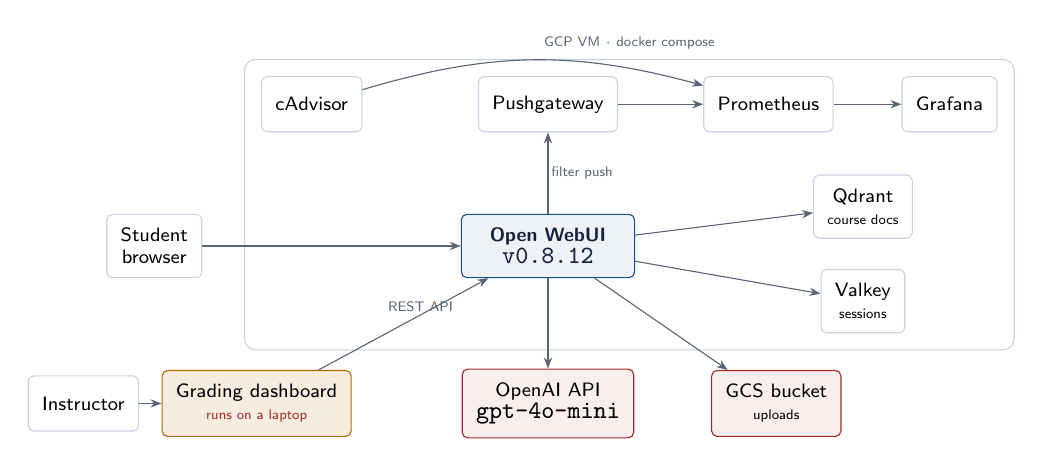
\begin{tikzpicture}[scale=1,every node/.style={transform shape}]
    % --- monitoring band
    \node[box]  at (3.9,4.7) (cad)  {cAdvisor};
    \node[box]  at (6.9,4.7) (pg)   {Pushgateway};
    \node[box]  at (9.7,4.7) (prom) {Prometheus};
    \node[box]  at (12.0,4.7)(graf) {Grafana};
    % --- application band
    \node[box]  at (1.9,2.9) (stu)  {Student\\browser};
    \node[core,minimum width=22mm] at (6.9,2.9) (ow) {Open WebUI\\ \code{v0.8.12}};
    \node[box]  at (10.9,3.4)(qd)   {Qdrant\\ {\tiny course docs}};
    \node[box]  at (10.9,2.2)(rd)   {Valkey\\ {\tiny sessions}};
    % --- external / instructor band
    \node[box,fill=ffcAmber!12,draw=ffcAmber] at (3.2,0.9) (dash)
      {Grading dashboard\\ \textcolor{ffcRed}{\tiny runs on a laptop}};
    \node[box]  at (1.0,0.9) (prof) {Instructor};
    \node[ext]  at (6.9,0.9) (oai)  {OpenAI API\\ \code{gpt-4o-mini}};
    \node[ext]  at (9.8,0.9) (gcs)  {GCS bucket\\ {\tiny uploads}};

    \draw[arr] (stu) -- (ow);
    \draw[arr] (ow) -- (qd);
    \draw[arr] (ow) -- (rd);
    \draw[arr] (ow) -- (oai);
    \draw[arr] (ow) -- (gcs);
    \draw[arr] (ow) -- node[lbl,right]{filter push} (pg);
    \draw[arr] (pg) -- (prom);
    \draw[arr] (cad) to[bend left=16] (prom);   % arc gently over Pushgateway
    \draw[arr] (prom) -- (graf);
    \draw[arr] (prof) -- (dash);
    \draw[arr] (dash) -- node[lbl,above,pos=0.6]{REST API} (ow);
    \begin{scope}[on background layer]
      \node[fit=(cad)(graf)(ow)(qd)(rd)(pg),draw=ffcRule,rounded corners,
            inner sep=6pt,label={[font=\tiny,text=ffcGrey]above:GCP VM $\cdot$ docker compose}] {};
    \end{scope}
  \end{tikzpicture}
  \end{center}
  \vspace{-0.4em}
  {\footnotesize Eight containers on one VM. Retrieval over course documents in Qdrant.
  Chat metrics pushed by a plugin. \bad{The grading dashboard is the outlier --- it is not hosted.}}
  \note{Walk the diagram left to right. Land on the one thing in amber: the professor's tool runs on a laptop. That is workstream A's headline problem.}
\end{frame}

%== 5 =========================================================================
\begin{frame}{The lesson that shaped this project}
  \vspace{-0.3em}
  \begin{columns}[T]
    \begin{column}{0.47\textwidth}
      \textbf{\bad{Before}} --- Spring 2026 and earlier
      \begin{center}
      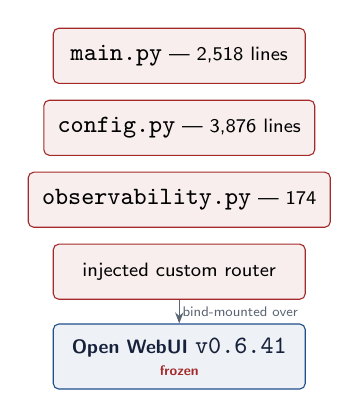
\begin{tikzpicture}
        \node[ext,minimum width=32mm] (a) {\code{main.py} --- 2{,}518 lines};
        \node[ext,minimum width=32mm,below=2mm of a] (b) {\code{config.py} --- 3{,}876 lines};
        \node[ext,minimum width=32mm,below=2mm of b] (c) {\code{observability.py} --- 174};
        \node[ext,minimum width=32mm,below=2mm of c] (d) {injected custom router};
        \node[core,minimum width=32mm,below=3mm of d] (e) {Open WebUI \code{v0.6.41}\\ \textcolor{ffcRed}{\tiny frozen}};
        \draw[arr] (d) -- node[lbl,right]{bind-mounted over} (e);
      \end{tikzpicture}
      \end{center}
      \vspace{2pt}
      {\footnotesize \bad{$\approx$6{,}500 lines} of forked vendor code, re-merged by hand
      on every upgrade. Users reached a feature via a \emph{browser bookmarklet}.}
    \end{column}
    \begin{column}{0.47\textwidth}
      \textbf{\good{After}} --- what we inherited
      \begin{center}
      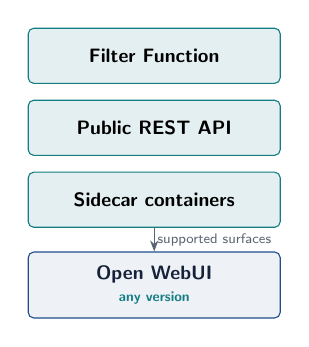
\begin{tikzpicture}
        \node[newb,minimum width=32mm] (f) {Filter Function};
        \node[newb,minimum width=32mm,below=2mm of f] (g) {Public REST API};
        \node[newb,minimum width=32mm,below=2mm of g] (h) {Sidecar containers};
        \node[core,minimum width=32mm,below=3mm of h] (i) {Open WebUI\\ \textcolor{ffcTeal}{\tiny any version}};
        \draw[arr] (h) -- node[lbl,right]{supported surfaces} (i);
      \end{tikzpicture}
      \end{center}
      \vspace{2pt}
      {\footnotesize The \code{Dockerfile} is now \good{one line}. Every customisation
      rides a documented plugin or API surface.}
    \end{column}
  \end{columns}
  \vspace{0.1em}
  \centerline{\small\textit{This is the previous team's real achievement --- and it is why this semester is possible.}}
  \note{Give the last team credit. Six and a half thousand lines of fork to get two features. The bookmarklet detail always lands -- mention it.}
\end{frame}

%== 6 =========================================================================
\begin{frame}{Where it still hurts}
  \vspace{0.2em}
  \begin{center}\footnotesize
  \begin{tabular}{p{5.6cm}p{6.6cm}}
    \toprule
    \textbf{Problem} & \textbf{Consequence} \\
    \midrule
    Pinned to \code{v0.8.12}; upstream ships \code{v0.11.x} & Three minor versions of fixes, features --- and \emph{migrations} --- deferred \\
    Metrics plugin is pasted into the admin UI by hand after every deploy & Deployment is not reproducible; metrics vanish silently \\
    That plugin is synchronous, with blocking network I/O and shared state & On the v0.9+ async core it degrades every concurrent user \\
    \bad{Grading dashboard is not hosted} & A professor needs SSH and a terminal to grade \\
    No CI, no automated smoke test & Past upgrades broke things silently \\
    No alerting on \code{/ready} & An outage was discovered from students \\
    Two RAG stacks, two scoring implementations & Ambiguity about which numbers are canonical \\
    Default \code{admin/admin}; unrotated leaked key & Straightforward security debt \\
    \bottomrule
  \end{tabular}
  \end{center}
  \vspace{0.4em}
  \centerline{\small None of this is exotic. It is the gap between \emph{a system that works} and \emph{a system you can hand over}.}
  \note{Read only three or four rows aloud -- hosted dashboard, no CI, version gap. Close with the "gap between works and handover" line.}
\end{frame}

%== 7 =========================================================================
\sectionslide{Workstream A}{Harden and modernise}{Weeks 1--15 $\cdot$ this must not slip}

%== 8 =========================================================================
\begin{frame}{The compatibility contract}
  \vspace{0.5em}
  \begin{block}{The rule}
    \normalsize Open WebUI is a \hl{dependency}, not a codebase we own. We must be able to
    pull any published release and have the platform work --- with no merge, no patch,
    no re-fork.
  \end{block}
  \vspace{0.6em}
  \begin{columns}[T]
    \begin{column}{0.55\textwidth}
      {\small Every feature must ride a surface that upstream \hl{publishes, documents,
      and versions}.\\[6pt]
      If a feature cannot be built that way, the \emph{feature} is redesigned or dropped.
      The core is never modified.}
    \end{column}
    \begin{column}{0.42\textwidth}
      \begin{block}{The one-sentence test}
        \small \textit{If upstream cut a release tomorrow and we ran it unchanged, would
        this still work?}\\[4pt]
        If the answer needs ``well, as long as they don't change\ldots'', it is forbidden.
      \end{block}
    \end{column}
  \end{columns}
  \note{Slow down here. This is the intellectual core of the deck. The one-sentence test is what they should apply in code review all semester.}
\end{frame}

%== 9 =========================================================================
\begin{frame}{Where we are allowed to build}
  \vspace{0.2em}
  \begin{center}\footnotesize
  \begin{tabular}{llp{6.4cm}}
    \toprule
    & \textbf{Surface} & \textbf{Use it for} \\
    \midrule
    A1 & Environment / admin settings & models, RAG parameters, STT and TTS engines, OTel export \\
    A2 & Filter Functions & observing or lightly rewriting a request in flight \\
    A3 & Pipe Functions & exposing our own logic as a selectable ``model'' \\
    A4 & Action Functions & per-message buttons --- e.g.\ \emph{start a voice session} \\
    A5 & Pipelines server & anything needing its own dependencies, GPU, or heavy compute \\
    A6 & Tools / OpenAPI / MCP & letting the model call our services \\
    A7 & Public REST API & grading extraction, KB sync, \hl{the avatar app} \\
    A8 & Sidecar containers & exporters, our own web applications \\
    A9 & Reverse-proxy composition & TLS, auth, path routing on one hostname \\
    A10 & Knowledge Bases and Skills & course documents and frameworks, professor-editable \\
    \bottomrule
  \end{tabular}
  \end{center}
  \vspace{0.3em}
  \centerline{\small\textbf{Heuristic:} needs to see \emph{inside} a request $\to$ A2--A4. Needs its own runtime $\to$ A5/A8, talking over A7.}
  \note{Do not read the table. Point at A7 and A8 -- those two are what the avatar work will use. The heuristic line is the takeaway.}
\end{frame}

%== 10 ========================================================================
\begin{frame}{What is forbidden --- permanently}
  \vspace{0.3em}
  \begin{center}\footnotesize
  \begin{tabular}{lp{5.9cm}p{5.0cm}}
    \toprule
    & \textbf{Forbidden} & \textbf{Why} \\
    \midrule
    F1 & Mounting or copying anything into \code{/app/backend/open\_webui/} & this \emph{is} the fork \\
    F2 & Adding modules to the \code{open\_webui} package & same, plus coupling to internals \\
    F3 & Building a custom image from modified source & tracks upstream by hand forever \\
    F4 & JavaScript injection into the Svelte frontend & no contract; breaks on any refactor \\
    F5 & Direct SQL against Open WebUI's schema & the schema is private, and \emph{did} change \\
    F6 & Monkeypatching internals from a Function & a fork wearing a plugin costume \\
    F7 & Relying on undocumented endpoints or fields & fine until it isn't; fails silently \\
    F8 & Pinning to an old release to dodge migration work & \bad{this is exactly how v0.6.41 happened} \\
    \bottomrule
  \end{tabular}
  \end{center}
  \vspace{0.4em}
  \centerline{\small It always starts the same way: \textit{``it's just one file, we'll mount it read-only.''}}
  \note{F6 and F8 are the ones teams actually violate. The closing quote is the warning to remember.}
\end{frame}

%== 11 ========================================================================
\begin{frame}{Audit: what we still have to strip out}
  \vspace{0.2em}
  {\footnotesize \good{Good news:} the active stack is already compliant --- no compose file
  mounts anything into Open WebUI's source tree. What remains is peripheral coupling and
  \emph{loaded guns left in the tree.}}
  \vspace{0.5em}
  \begin{center}\footnotesize
  \begin{tabular}{lp{4.8cm}p{5.2cm}l}
    \toprule
    & \textbf{Finding} & \textbf{Action} & \textbf{Risk} \\
    \midrule
    C-1 & the vendor-fork source under \code{legacy/} --- with a README telling you how to re-fork & delete from the tree; leave a tombstone pointing at the commit & \bad{High} \\
    C-2 & \code{--legacy} direct-SQLite flag (a \code{TODO} stub) & delete the flag; REST API is the only path & Med \\
    C-3 & custom \code{build:} context for Open WebUI & replace with a pinned \code{image:}; delete the \code{Dockerfile} & Low \\
    C-4 & metrics filter: sync, blocking I/O, shared state & rewrite async, or retire it for native OTel & \bad{High} \\
    C-6 & \code{:latest} images (Qdrant, cAdvisor) & pin every image & Med \\
    C-7 & Grafana 9.0.0, default \code{admin/admin} & upgrade; remove the default password & \bad{High} \\
    C-8/9 & two RAG stacks, two scoring implementations & pick one canonical each, in writing & Med \\
    C-10 & previously leaked provider key not yet rotated & rotate at the provider; add \code{gitleaks} to CI & \bad{High} \\
    \bottomrule
  \end{tabular}
  \end{center}
  \note{C-1 is the headline: the repo still contains working instructions for re-creating the fork. Deleting it is a five-minute job with outsized value.}
\end{frame}

%== 12 ========================================================================
\begin{frame}{Version debt: what three releases cost us}
  \vspace{0.4em}
  \begin{center}\small
  \begin{tabular}{lp{3.7cm}p{7.0cm}}
    \toprule
    \textbf{Release} & \textbf{Change} & \textbf{What it means for us} \\
    \midrule
    \code{v0.9.0} & backend went \hl{async top to bottom} & \bad{our Filter Function must be migrated} --- sync plugin code with blocking I/O is now actively harmful \\[4pt]
    \code{v0.10.0} & \code{config} table replaced by a per-key table & \bad{one-way migration.} An older instance pointed at a migrated database fails immediately \\[4pt]
    \code{v0.11.0} & additive columns only; \code{psycopg} v3; major UI reorganisation & low migration risk, \hl{high documentation risk} --- every screenshot and click-path we publish is now wrong \\
    \bottomrule
  \end{tabular}
  \end{center}
  \vspace{0.7em}
  \centerline{\small We are on \code{v0.8.12}. \textbf{The longer this waits, the more expensive it gets ---}}
  \centerline{\small\textit{which is precisely the dynamic that produced the v0.6.41 freeze.}}
  \note{The point is not "upgrades are nice". It is that deferred migrations compound, and this project already has the scar to prove it.}
\end{frame}

%== 13 ========================================================================
\begin{frame}{How we will do the upgrade}
  \vspace{0.4em}
  \begin{columns}[T]
    \begin{column}{0.56\textwidth}
      \small
      \begin{enumerate}
        \item Snapshot production --- and \hl{restore the snapshot into the test stack}.
              \textit{A backup you have never restored is not a backup.}
        \item Upgrade the test stack first, on real production data.
        \item Move \hl{one minor version at a time}: 0.8 $\to$ 0.9 $\to$ 0.10 $\to$ 0.11.
              Migrations run sequentially; a single jump makes failures unattributable.
        \item Run the smoke suite at every step. Write the runbook \emph{as you go}.
        \item Decide \hl{SQLite $\to$ PostgreSQL} explicitly, and record the decision either way.
        \item Schedule the production window with the rollback written \emph{before} you start.
        \item Re-shoot every screenshot for the new UI.
      \end{enumerate}
    \end{column}
    \begin{column}{0.40\textwidth}
      \begin{block}{Done when}
        \small
        Production runs the current release.\\[3pt]
        The runbook exists \emph{and was followed}.\\[3pt]
        The smoke suite passes.\\[3pt]
        Docs match what a user actually sees.\\[3pt]
        The rollback is \hl{proven}, not theorised.
      \end{block}
      \vspace{0.4em}
      {\footnotesize \bad{Schedule this outside student deadline weeks.}}
    \end{column}
  \end{columns}
  \note{Step 1 and step 6 are the professional habits worth arguing for. Most teams skip both and get away with it until they don't.}
\end{frame}

%== 14 ========================================================================
\begin{frame}{CI/CD --- and the guard that keeps the fork dead}
  \vspace{0.3em}
  \begin{columns}[T]
    \begin{column}{0.52\textwidth}
      \textbf{\color{ffcBlue}Pipeline, by value per hour spent}
      \begin{enumerate}\small
        \item \textbf{Smoke test on every push} --- bring the stack up, wait for
              \code{/health} then \code{/ready}, send a chat completion, upload a
              document, assert retrieval returns it
        \item \textbf{Fork guard} (below)
        \item \textbf{Secret scanning} --- \code{gitleaks}, including history
        \item \textbf{Lint and unit tests} --- especially on the scoring service:
              \emph{it produces numbers that become grades}
        \item \textbf{Deploy on tag} --- pull, restart, re-smoke, auto-rollback
      \end{enumerate}
    \end{column}
    \begin{column}{0.45\textwidth}
      \begin{block}{The fork guard --- fails the build when\ldots}
        \small
        a compose file mounts into \code{open\_webui/}\\[2pt]
        the image is built from modified source\\[2pt]
        Python opens SQLite against Open WebUI's data\\[2pt]
        \code{gitleaks} finds a credential\\[2pt]
        any image reference ends in \code{:latest}
      \end{block}
      \vspace{0.3em}
      {\footnotesize $\approx$40 lines of grep and one GitHub Action. \hl{This is what makes
      the policy real instead of aspirational.} Build it in Week 2.}
    \end{column}
  \end{columns}
  \note{Emphasise: a policy nobody enforces is a wish. Forty lines of grep converts a document into a constraint.}
\end{frame}

%== 15 ========================================================================
\begin{frame}{Two fixes that change who can use this}
  \vspace{0.4em}
  \begin{columns}[T]
    \begin{column}{0.47\textwidth}
      \textbf{\color{ffcBlue}Host the grading dashboard}\\[4pt]
      {\small Today a professor must SSH into a GCP VM and run a shell script.\\[5pt]
      Containerise the backend, build the frontend to static assets, put Nginx in front with
      TLS and real authentication, and give them a \hl{URL}.\\[5pt]
      \textit{Watch:} make \code{/refresh} asynchronous with visible progress --- it scores
      every question through a paid API.}
      \\[6pt]
      {\footnotesize\good{Done when} a professor grades with no terminal, no VPN, and no help
      from a student.}
    \end{column}
    \begin{column}{0.47\textwidth}
      \textbf{\color{ffcBlue}Observability without manual steps}\\[4pt]
      {\small Chat metrics currently depend on a human pasting Python into an admin form
      after every deployment.\\[5pt]
      Fix the \emph{class} of problem: enable Open WebUI's \hl{native OpenTelemetry export}
      into a collector, and scrape that. Then retire the filter --- or rewrite it async.\\[5pt]
      Add a \code{/ready} uptime check that alerts \emph{a person}, and a memory alert as a
      leading indicator.}
      \\[6pt]
      {\footnotesize\good{Done when} a clean deployment produces metrics with zero manual
      steps, and an induced outage pages someone in five minutes.}
    \end{column}
  \end{columns}
  \note{These two are the highest-adoption-value items in the whole plan. The dashboard one is the difference between a tool that gets used and one that doesn't.}
\end{frame}

%== 16 ========================================================================
\begin{frame}{Remove the ambiguity}
  \vspace{0.5em}
  \begin{columns}[T]
    \begin{column}{0.31\textwidth}
      \begin{block}{Scoring exists twice}
        \small JavaScript and Python, kept in sync by hand.\\[4pt]
        Declare \hl{Python canonical}. Retire the prototype. Add tests that pin the rubric
        arithmetic and ABI weights.
      \end{block}
    \end{column}
    \begin{column}{0.31\textwidth}
      \begin{block}{RAG exists twice}
        \small Native Qdrant (what students use) and a standalone ChromaDB pipeline
        (which nothing uses).\\[4pt]
        Retire it, or promote it behind a \hl{Pipelines server}. Decide in writing.
      \end{block}
    \end{column}
    \begin{column}{0.31\textwidth}
      \begin{block}{Extraction is heuristic}
        \small Student questions are found by punctuation and keywords.\\[4pt]
        \hl{Measure its accuracy} against a hand-labelled sample before trusting the scores
        built on top of it.
      \end{block}
    \end{column}
  \end{columns}
  \vspace{0.9em}
  \centerline{\small Each of these will eventually produce a wrong answer that nobody can explain.}
  \centerline{\small\textit{Dead code with live bugs is a tax --- the citation bug we fixed lived in the stack nobody runs.}}
  \note{The third column is the sleeper. If question extraction is 70 percent accurate, every grade downstream inherits that error, silently.}
\end{frame}

%== 17 ========================================================================
\sectionslide{Workstream B}{Embodied advising}{The new research track $\cdot$ Weeks 3--15}

%== 18 ========================================================================
\begin{frame}{Why typing is not enough}
  \vspace{0.2em}
  \begin{columns}[T]
    \begin{column}{0.5\textwidth}
      {\small FIN 602 exists to prepare students for \hl{a room with a real family in it}.
      \\[8pt]
      That room demands: listening while someone is still talking, hearing hesitation,
      holding eye contact through an uncomfortable question about money, and asking the
      follow-up \emph{out loud} --- without a backspace key.}
    \end{column}
    \begin{column}{0.46\textwidth}
      \begin{block}{The gap}
        \small The platform teaches the \emph{content} of good advising well.\\[4pt]
        It cannot teach the \emph{performance} of it --- because typing removes every one of
        those pressures.\\[4pt]
        A student can draft, delete, and reword for ninety seconds before asking
        \textit{``what happens to the business if something happens to you?''}
      \end{block}
    \end{column}
  \end{columns}
  \vspace{0.8em}
  \begin{block}{This semester's hypothesis --- and it is a hypothesis}
    \small A spoken, face-to-face AI client produces meaningfully better preparation than a
    text chatbot --- and we can \hl{measure whether that is true} with the scoring pipeline
    the platform already has. This track is designed to be allowed to answer \emph{no}.
  \end{block}
  \note{This is the emotional centre of the pitch. Deliver the backspace-key line slowly. Then immediately frame it as testable, not assumed.}
\end{frame}

%== 19 ========================================================================
\begin{frame}{What we are actually building}
  \vspace{0.5em}
  {\small A student opens a link, sees a face, and says out loud:}
  \vspace{0.3em}
  \begin{center}
    \colorbox{ffcMist}{\parbox{0.8\textwidth}{\vspace{3pt}\small\itshape\centering
    ``Hi --- I'm going to ask you a few questions about your family's finances.
    Is that alright?''\vspace{3pt}}}
  \end{center}
  \vspace{0.3em}
  {\small The client on screen \hl{looks at them, nods, and answers in their own voice},
  in character, with their own financial situation --- drawn from the same course documents
  the text bot already uses.\\[4pt]
  If the student interrupts, the client \hl{stops talking}. If the student goes quiet, the
  client waits --- and may eventually prompt them, the way a real, slightly impatient client
  would.\\[4pt]
  At the end, the transcript lands in \hl{the same grading dashboard}, scored on the same
  seven dimensions and the same ABI rubric.}
  \vspace{0.5em}
  \begin{block}{What we are \emph{not} building}
    \small A photorealistic digital human. A likeness of any real person. A replacement for
    the text interface --- text stays. Voice and face are an \emph{additional mode}.
  \end{block}
  \note{Read the quoted line as if speaking to the avatar. The "stops talking" detail is what separates a real prototype from a demo video.}
\end{frame}

%== 20 ========================================================================
\begin{frame}{The constraint dictates the architecture}
  \vspace{0.5em}
  {\small The instinct is to put the avatar \emph{inside} the Open WebUI chat window.}
  \vspace{0.4em}
  \begin{block}{That is forbidden --- F3 and F4 at once}
    \small Open WebUI's frontend is a Svelte application we do not own. Embedding a WebRTC
    video pane in it means forking and re-merging that frontend forever ---
    \bad{precisely the mistake this project spent a semester undoing.}
  \end{block}
  \vspace{0.5em}
  {\small So the constraint decides the design, and the design it produces is \good{better}:}
  \vspace{0.3em}
  \centerline{\small\textbf{The avatar is a companion web application in its own container.}}
  \centerline{\small Open WebUI stays the \hl{brain} (model, RAG, knowledge) and the
  \hl{system of record} (transcripts). We talk to it over the public API.}
  \vspace{0.6em}
  \begin{columns}[T]
    \begin{column}{0.49\textwidth}
      {\footnotesize \good{$\rightarrow$} deploy, roll back, and load-test independently\\
      \good{$\rightarrow$} survives every upstream release by construction}
    \end{column}
    \begin{column}{0.49\textwidth}
      {\footnotesize \good{$\rightarrow$} if we kill the track in December, we delete one container\\
      \good{$\rightarrow$} students and professors keep the interface they know}
    \end{column}
  \end{columns}
  \note{This slide is the argument that the compatibility policy is not bureaucracy -- it produced a better architecture than the instinctive one.}
\end{frame}

%== 21 ========================================================================
\begin{frame}{Reference architecture}
  \vspace{-0.3em}
  \begin{center}
  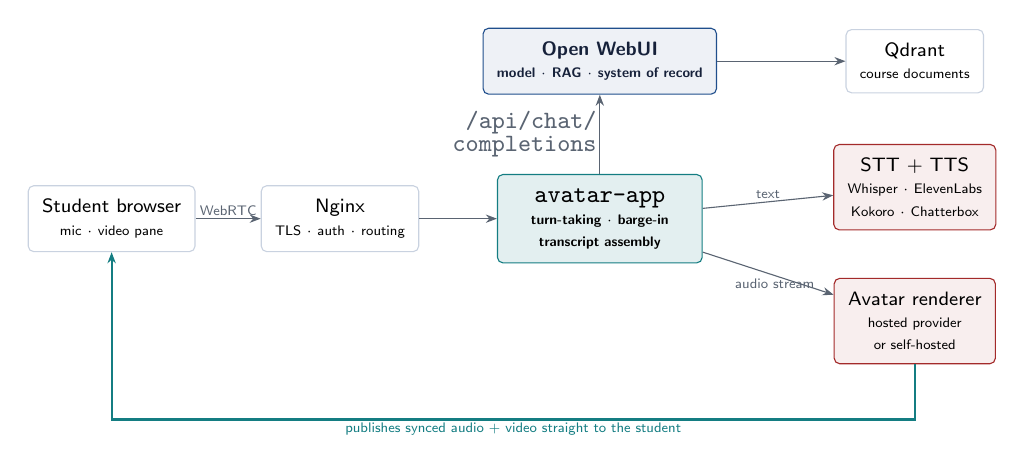
\begin{tikzpicture}[scale=1,every node/.style={transform shape}]
    \node[box]  at (1.7,3.0) (br)  {Student browser\\ {\tiny mic $\cdot$ video pane}};
    \node[box]  at (4.6,3.0) (px)  {Nginx\\ {\tiny TLS $\cdot$ auth $\cdot$ routing}};
    \node[newb,minimum width=26mm] at (7.9,3.0) (app)
        {\code{avatar-app}\\ {\tiny turn-taking $\cdot$ barge-in}\\ {\tiny transcript assembly}};
    \node[core,minimum width=26mm] at (7.9,5.0) (ow)
        {Open WebUI\\ {\tiny model $\cdot$ RAG $\cdot$ system of record}};
    \node[box]  at (11.9,5.0) (qd) {Qdrant\\ {\tiny course documents}};
    \node[ext]  at (11.9,3.4) (stt) {STT + TTS\\ {\tiny Whisper $\cdot$ ElevenLabs}\\ {\tiny Kokoro $\cdot$ Chatterbox}};
    \node[ext]  at (11.9,1.7) (av)  {Avatar renderer\\ {\tiny hosted provider}\\ {\tiny or self-hosted}};

    \draw[arr] (br) -- node[lbl,above]{WebRTC} (px);
    \draw[arr] (px) -- (app);
    \draw[arr] (app) -- node[lbl,left,align=right]{\code{/api/chat/}\\ \code{completions}} (ow);
    \draw[arr] (ow) -- (qd);
    \draw[arr] (app) -- node[lbl,above]{text} (stt);
    \draw[arr] (app) -- node[lbl,below,pos=0.55]{audio stream} (av);
    \draw[arr,draw=ffcTeal,thick] (av.south) -- ++(0,-0.7)
        -| node[lbl,below,pos=0.25,text=ffcTeal]
        {publishes synced audio + video straight to the student} (br.south);
  \end{tikzpicture}
  \end{center}
  \vspace{-0.2em}
  {\footnotesize \good{The pattern that matters:} the renderer is not a step we wait on. It
  \hl{joins the session as its own participant} --- we stream it audio, and it publishes
  finished, lip-synced video directly to the student. That removes a full round trip through
  our server. It is the difference between a video call and a laggy video attachment.}
  \note{Trace the teal arrow. Do not hand-roll WebRTC and turn-taking -- use LiveKit Agents or Pipecat. That is not the semester's research question.}
\end{frame}

%== 22 ========================================================================
\begin{frame}{Latency is the number that decides everything}
  \vspace{0.3em}
  \begin{columns}[T]
    \begin{column}{0.55\textwidth}
      \centering\footnotesize
      \begin{tabular}{lr}
        \toprule
        \textbf{Stage} & \textbf{Realistic} \\
        \midrule
        Voice activity detection / endpointing & 150--300\,ms \\
        Speech to text & 150--300\,ms \\
        \textcolor{ffcRed}{Retrieval (RAG)} & \textcolor{ffcRed}{100--300\,ms} \\
        LLM time-to-first-token & 300--600\,ms \\
        Text to speech, first byte & 150--300\,ms \\
        Avatar render + network & 200--500\,ms \\
        \midrule
        \textbf{First audible syllable} & \textbf{1.0--2.3\,s} \\
        \bottomrule
      \end{tabular}
    \end{column}
    \begin{column}{0.42\textwidth}
      \begin{block}{Targets for this semester}
        \small p50 under \hl{1.2\,s}\\
        p95 under \hl{2.0\,s}\\
        barge-in interrupts within \hl{300\,ms}
      \end{block}
      \vspace{0.3em}
      {\footnotesize Conversation tolerates about a second. Past two, a person stops feeling
      \emph{heard} and starts feeling \emph{processed}.}
    \end{column}
  \end{columns}
  \vspace{0.5em}
  {\footnotesize \bad{The RAG trap:} the text platform retrieves on every turn. In a spoken
  loop that sits directly in the critical path. Strongly consider loading the family scenario
  into the system prompt \emph{once} at session start --- a 2{,}000-token persona brief costs
  less latency than a vector search per turn, every turn.\\[3pt]
  \hl{Instrument every stage separately, in Week 5.} One end-to-end number tells you it is
  slow, not what to fix.}
  \note{The RAG trap is the most useful engineering insight on this slide -- it is counterintuitive and it is where a naive implementation loses half a second per turn.}
\end{frame}

%== 23 ========================================================================
\begin{frame}{Three strategies --- and the one we start with}
  \vspace{0.3em}
  \begin{columns}[T]
    \begin{column}{0.31\textwidth}
      \begin{block}{1. Hosted streaming}
        \footnotesize HeyGen LiveAvatar, Tavus (Phoenix-4), Simli, Anam, bitHuman, Beyond
        Presence, D-ID.\\[4pt]
        Plug into LiveKit or Pipecat; swap providers behind one interface.\\[4pt]
        \textbf{Vendor latency claims are measured under vendor conditions.}
        \hl{Measuring ours is the assignment.}
      \end{block}
    \end{column}
    \begin{column}{0.31\textwidth}
      \begin{block}{2. Self-hosted open source}
        \footnotesize Whisper $\to$ open TTS $\to$ an open lip-sync renderer.\\[4pt]
        \good{For:} no per-minute cost, no student audio leaving our infrastructure.\\[4pt]
        \bad{Against:} needs a GPU we do not have; quality and latency lag; it becomes an
        infrastructure project.
      \end{block}
    \end{column}
    \begin{column}{0.31\textwidth}
      \begin{block}{3. Voice only --- no face}
        \footnotesize Open WebUI \emph{already has} hands-free call mode. STT and TTS are
        configuration, not engineering.\\[4pt]
        Captures much of the benefit --- speaking aloud, no backspace, real-time pressure ---
        at \hl{near-zero build cost}.
      \end{block}
    \end{column}
  \end{columns}
  \vspace{0.7em}
  \begin{block}{Start with \#3, in Week 3}
    \small It de-risks the entire track. If avatars prove too slow, too costly, or too
    fragile, \hl{the course still gains spoken practice this semester.} B0 ships regardless.
  \end{block}
  \note{The strategic point: build the fallback first, and build it in three weeks. That is how you make an ambitious research track safe to attempt.}
\end{frame}

%== 24 ========================================================================
\begin{frame}{What it costs --- and how we stop it running away}
  \vspace{0.4em}
  \begin{columns}[T]
    \begin{column}{0.52\textwidth}
      \centering\footnotesize
      40 students $\times$ 4 sessions $\times$ 15 min $=$ \textbf{40 hours / semester}
      \vspace{0.4em}
      \begin{tabular}{lr}
        \toprule
        \textbf{Line item} & \textbf{Semester} \\
        \midrule
        Avatar streaming ($\sim$\$0.10--0.20/min) & \$240--480 \\
        Speech to text & \$10--30 \\
        Text to speech & \$20--60 \\
        LLM (short spoken turns) & \$15--40 \\
        \midrule
        \textbf{Total} & \textbf{$\approx$\$285--610} \\
        \bottomrule
      \end{tabular}
      \vspace{0.3em}
      {\tiny Checked August 2026. Prices move quarterly --- re-derive at signup and record the date.}
    \end{column}
    \begin{column}{0.45\textwidth}
      \begin{block}{Controls from day one --- not after the first bill}
        \small
        15-minute hard cap, enforced server-side\\[3pt]
        per-student session quota\\[3pt]
        billing alert at 50\% of budget\\[3pt]
        sessions terminate on disconnect\\[3pt]
        a kill switch that needs no redeploy
      \end{block}
      \vspace{0.3em}
      {\footnotesize \bad{Do the arithmetic before advocating self-hosting:} an L4-class GPU
      VM is roughly \$500/month if left running. At 40 hours a semester, \hl{buying beats
      building.} Self-hosting wins on privacy and at scale --- not on cost, here.}
    \end{column}
  \end{columns}
  \note{The self-hosting arithmetic is the slide's punchline. Students instinctively assume open source is cheaper; at this volume it is roughly ten times more expensive.}
\end{frame}

%== 25 ========================================================================
\begin{frame}{How we will evaluate it honestly}
  \vspace{0.3em}
  {\small \good{We already own the outcome measure} --- so use it. Within-subjects,
  counterbalanced: each student practises in two or three modalities with matched scenarios,
  in varied order.}
  \vspace{0.5em}
  \begin{center}\footnotesize
  \begin{tabular}{lp{6.6cm}}
    \toprule
    \textbf{Measure} & \textbf{Question it answers} \\
    \midrule
    7-dimension question quality & do students ask \emph{better} questions when speaking? \\
    ABI trust scores & does modality change how the interaction reads? \\
    Questions asked; session duration & does speaking increase or suppress engagement? \\
    \textcolor{ffcTeal}{Interruptions; talk-time ratio} & \textcolor{ffcTeal}{are students learning to \emph{listen}?} \\
    Hesitation before sensitive questions & does rehearsal reduce discomfort over sessions? \\
    Realism, social presence, anxiety (survey) & is it believable and productive --- or uncanny? \\
    \bottomrule
  \end{tabular}
  \end{center}
  \vspace{0.5em}
  {\footnotesize \bad{Do not over-claim.} The sample is small and the semester is short.
  \textit{``Twelve students, counterbalanced, with these effect sizes and confidence
  intervals''} is a credible result. \textit{``Avatars improve learning''} is not.
  \hl{A well-designed study with an honest negative result is the better deliverable} --- and
  it will be graded that way.}
  \note{The teal row is the genuinely novel contribution: whether a student lets the client finish talking may be a better measure of advising skill than anything the current rubric captures.}
\end{frame}

%== 26 ========================================================================
\begin{frame}{Phases and gates}
  \vspace{0.1em}
  \begin{center}\small
  \begin{tabular}{llp{6.0cm}p{3.6cm}}
    \toprule
    & \textbf{Weeks} & \textbf{Deliverable} & \textbf{Gate} \\
    \midrule
    \textbf{B0} & 3--5 & hands-free spoken practice on Open WebUI's own call mode & \emph{ships regardless} \\[3pt]
    \textbf{B1} & 4--7 & two providers behind one interface, measured on latency, cost, barge-in & \hl{choose --- or recommend stopping} \\[3pt]
    \textbf{B2} & 7--12 & \code{avatar-app} container; transcripts written back into grading & \hl{five students complete a full session} \\[3pt]
    \textbf{B3} & 11--15 & text vs voice vs avatar, measured on the existing rubric & \hl{evidence-backed go / no-go} \\
    \bottomrule
  \end{tabular}
  \end{center}
  \vspace{0.3em}
  \begin{block}{The gates are real}
    \small ``Stop'' is an acceptable outcome at every gate. \bad{``We didn't measure'' is not.}\\[4pt]
    And build the transcript write-back \emph{first} in B2, not last --- an avatar session that
    never reaches the grading dashboard is a demo, not a feature.
  \end{block}
  \note{Make the kill switch explicit and unembarrassing. Research tracks that cannot fail are not research tracks.}
\end{frame}

%== 27 ========================================================================
\begin{frame}{Ethics, privacy, and consent --- settle this in Week 2}
  \vspace{0.4em}
  \begin{columns}[T]
    \begin{column}{0.48\textwidth}
      \small
      \begin{itemize}
        \item Student transcripts are \hl{education records} under FERPA. Adding audio adds a
              biometric-adjacent identifier to that.
        \item \hl{Written informed consent} before any recording: what is captured, where it
              lives, how long, who sees it, how to opt out --- \textbf{without affecting a grade}.
        \item \bad{No likeness of any real person.} Use provider stock avatars under licence.
              Do not clone a professor's face or voice ``as a joke.''
      \end{itemize}
    \end{column}
    \begin{column}{0.48\textwidth}
      \small
      \begin{itemize}
        \item \hl{Disclose the AI.} We are teaching advising, not testing whether students can
              be fooled.
        \item \hl{Minimise data.} Prefer keeping the transcript and discarding the audio.
        \item \hl{Read the vendor's terms} before sending one student's voice: retention,
              training use, sub-processors, region. For an education platform this can
              outweigh a latency win.
        \item Ask about \hl{IRB review} in Week 2 --- approval takes longer than you think.
      \end{itemize}
    \end{column}
  \end{columns}
  \vspace{0.5em}
  \centerline{\small\textit{Settle these before the data exists --- not in Week 13, when it already does.}}
  \note{Do not rush this slide. For a university deployment it is the one that determines whether the project is allowed to run at all.}
\end{frame}

%== 28 ========================================================================
\sectionslide{Execution}{Timeline, roles, and risk}{How the two tracks stay in balance}

%== 29 ========================================================================
\begin{frame}{The semester}
  \vspace{0.2em}
  \begin{center}\scriptsize
  \begin{tabular}{clp{4.9cm}p{4.9cm}}
    \toprule
    \textbf{Wk} & \textbf{Starts} & \textbf{Workstream A --- platform} & \textbf{Workstream B --- avatars} \\
    \midrule
    1 & Aug 24 & set up; run the stack; read the handoff & scope the landscape \\
    2 & Aug 31 & \hl{CI skeleton + fork guard + gitleaks} & requirements; \bad{consent and IRB questions} \\
    3 & Sep 7 & snapshot production; restore into test & \hl{B0: voice session end to end} \\
    4 & Sep 14 & test stack to v0.9.x; migrate the filter & provider shortlist; cost model \\
    5 & Sep 21 & v0.10.x on test & \hl{B0 demo}; latency baseline measured \\
    6 & Sep 28 & v0.11.x on test; docs re-shot & provider \#1 in a bare harness \\
    7 & Oct 5 & \hl{production upgrade window} & provider \#2; head-to-head \\
    8 & Oct 12 & hosted dashboard: container, proxy, TLS & \hl{Gate 1 --- pick, or stop} \\
    9 & Oct 19 & dashboard auth; professor walkthrough & companion app skeleton \\
    10 & Oct 26 & OTel + alerting live & avatar joins the session; barge-in works \\
    11 & Nov 2 & scoring consolidation + tests & transcript write-back \\
    12 & Nov 9 & RAG decision executed & \hl{Gate 2 --- five real sessions} \\
    13 & Nov 16 & performance and cost review & evaluation sessions run \\
    14 & Nov 23 & \textit{(short week)} runbooks and documentation & data analysed \\
    15 & Nov 30 & freeze; handoff written & recommendation drafted \\
    16 & Dec 7 & \multicolumn{2}{l}{\hl{final presentation and handoff}} \\
    \bottomrule
  \end{tabular}
  \end{center}
  \note{Point at weeks 2, 7, and 8. A and B are deliberately interleaved so neither starves. The upgrade lands before the avatar work gets heavy.}
\end{frame}

%== 30 ========================================================================
\begin{frame}{Who owns what}
  \vspace{0.5em}
  \begin{center}\small
  \begin{tabular}{lp{6.9cm}c}
    \toprule
    \textbf{Role} & \textbf{Owns} & \textbf{Track} \\
    \midrule
    Platform / DevOps lead & compose stack, upgrade path, CI/CD, proxy, secrets, backups & A \\
    Backend / integrations & grading service, extraction, scoring, Pipelines & A \\
    Realtime / avatar engineer & STT $\to$ LLM $\to$ TTS $\to$ avatar, latency, provider SDKs & B \\
    Frontend / UX & hosted dashboard, avatar app, session flow & A + B \\
    Data / assessment & evaluation design, metrics, transcript merge, outcomes & A + B \\
    \bottomrule
  \end{tabular}
  \end{center}
  \vspace{0.8em}
  \begin{block}{One duty every member carries}
    \small Review every pull request against the compatibility policy. The question is fixed:\\
    \centerline{\textit{``Which extension surface --- and what happens on the next upstream release?''}}
  \end{block}
  \vspace{0.3em}
  {\footnotesize On a smaller team one person holds two roles. \hl{The roles still exist, and so does the accountability.}}
  \note{Roles are about accountability, not headcount. The shared review duty is what keeps the policy alive when the deadline pressure arrives.}
\end{frame}

%== 31 ========================================================================
\begin{frame}{What could go wrong}
  \vspace{0.2em}
  \begin{center}\footnotesize
  \begin{tabular}{p{5.4cm}cp{5.6cm}}
    \toprule
    \textbf{Risk} & \textbf{Sev} & \textbf{Mitigation} \\
    \midrule
    The v0.10 config migration corrupts production data & \bad{High} & rehearse on a restored snapshot; verify the restore \emph{first}; run outside deadline weeks \\
    \bad{The avatar absorbs the semester and the platform work slips} & \bad{High} & A1 and A2 land before Week 8 --- the timeline front-loads them deliberately \\
    Avatar latency lands at 3+ seconds & Med & measure in Week 5; B0 voice-only ships regardless \\
    Streaming costs surprise the department & Med & caps, quotas, and a billing alarm from day one \\
    Voice and video create privacy exposure & \bad{High} & consent, no real likenesses, documented retention, sign-off \\
    A provider reprices or deprecates mid-semester & Med & provider-agnostic interface; keep the runner-up warm \\
    Somebody proposes embedding video in the chat page & Med & \bad{policy F3/F4 --- refuse.} The companion app exists for this reason \\
    Knowledge is lost at handoff, again & Med & \code{HANDOFF.md} updated continuously, not written in Week 15 \\
    \bottomrule
  \end{tabular}
  \end{center}
  \note{Row two is the one to dwell on. The exciting track will try to eat the boring track, and the boring track is what the course actually depends on.}
\end{frame}

%== 32 ========================================================================
\begin{frame}{Done means done}
  \vspace{0.5em}
  {\small The semester is complete when \hl{all eight} are true:}
  \vspace{0.4em}
  \begin{columns}[T]
    \begin{column}{0.48\textwidth}
      \small
      \begin{enumerate}
        \item Production runs a current release, upgraded via a written, \emph{rehearsed} runbook.
        \item A push runs CI; a tag deploys; a red build blocks the merge.
        \item The fork guard exists and passes --- and no re-forking instructions remain in the tree.
        \item A professor grades from an authenticated URL, with no terminal.
      \end{enumerate}
    \end{column}
    \begin{column}{0.48\textwidth}
      \small
      \begin{enumerate}
        \setcounter{enumi}{4}
        \item Metrics and alerting work from a clean deployment, with zero manual steps.
        \item Scoring and retrieval each have one canonical implementation, with tests.
        \item A working avatar prototype exists, real students used it, and a written
              evaluation backs a go/no-go call.
        \item \code{HANDOFF.md} lets the next team start in Week 1 --- not Week 4.
      \end{enumerate}
    \end{column}
  \end{columns}
  \note{Read these as acceptance criteria, not aspirations. Every one is verifiable by someone who was not in the room.}
\end{frame}

%== 33 ========================================================================
\begin{frame}[plain]
  \begin{tikzpicture}[remember picture,overlay]
    \fill[ffcInk] (current page.south west) rectangle (current page.north east);
    \node[anchor=west,text width=0.82\paperwidth] at ([xshift=1.2cm,yshift=1.5cm]current page.west)
      {\color{white}\LARGE\bfseries The goal is not to finish\\[6pt] FamilyFinanceChat.};
    \node[anchor=west,text width=0.78\paperwidth] at ([xshift=1.2cm,yshift=-0.5cm]current page.west)
      {\color{ffcRule}\large It is to leave a system where the interesting work is
       \textbf{\color{white}the pedagogy}, not \textbf{\color{white}the plumbing}.};
    \node[anchor=west,text width=0.78\paperwidth] at ([xshift=1.2cm,yshift=-2.3cm]current page.west)
      {\color{ffcGrey}\small Every hour spent this semester on upgrades, CI, and hosting is an
       hour a future team does not spend re-learning why the fork was a mistake.};
    \node[anchor=south east] at ([xshift=-1.2cm,yshift=0.9cm]current page.south east)
      {\color{ffcTeal}\small\bfseries Questions?};
  \end{tikzpicture}
  \note{Close on purpose, not on tasks. Then open the floor -- expect questions on avatar cost, on privacy, and on whether the upgrade can wait. It cannot.}
\end{frame}

\end{document}
